
%\documentclass[DIV19]{scrartcl}
%\usepackage[paper size={90mm, 120mm},left=2mm,right=2mm,top=2mm,bottom=2mm,nohead]{geometry}
% FIXME try prettyref
\documentclass[oneside,a4paper,12pt,BCOR20mm,DIV14]{scrbook}
%\documentclass{book}
% this gives a bit more than 2cm margin right and 4cm left
% koma-script.pdf: A4 is 210mmx297mm, BCOR is substraced before the page
% width is divided into DIV parts (HLU), a one sided leaves 1.5 HLU
% HLU*DIV=210-BCOR -> DIV=(210-BCOR)/HLU
% I want BCOR= 20mm 1.5 HLU = 20 mm 
% -> DIV=truncate(190*1.5/20) = truncate(14.25)=14
% I could use headinclude so that the header isn't printed into the margin

% Initially two softbound theses should be submitted to the
% Examinations Office for the examiners. Softbound theses should have
% the pages glued in.
% They don't need gold lettering on the spine.

\usepackage[utf8]{inputenc}
%\usepackage[T1]{fontenc}
\usepackage[usenames,dvipsnames]{color}
\usepackage[onehalfspacing]{setspace} 
\usepackage{graphicx}
\usepackage{longtable}
\usepackage{float}
\usepackage{wrapfig}
\usepackage{soul}
\usepackage{amssymb}
\usepackage{amsmath}

\usepackage[hypertex,breaklinks]{hyperref} % breaklinks only seems to
                                           % work with dvipdfm,
                                           % otherwise urls have no
                                           % line breaks
\usepackage{units}
\usepackage[disable]{todonotes} % for draft, disable for final
\usepackage{refcheck} % for draft, uncomment for final
\usepackage{lineno}
\usepackage{nomencl}
%\special{background Black}\special{color Green}
%\usepackage[utf8x]{inputenc} 
%\usepackage[T2A]{fontenc} % for the russian reference
\usepackage{wasysym} %diameter
% http://www.andy-roberts.net/misc/latex/latextutorial3.html

%\usepackage{url} % natbib.pdf p.11 break urls up, seems to be done
                 % with hyperref, though

\usepackage{natbib}


% for app_hilo
\usepackage{listings}
\usepackage{color}
\usepackage{textcomp}
\usepackage{subfigure}

% \listfiles % show which files are loaded by tex

\bibpunct{(}{)}{;}{a}{}{,}
\makenomenclature
\newcommand{\vect}[1]{\mathbf{#1}}
\renewcommand{\r}{\vect r}
\renewcommand{\a}{\vect a}
\newcommand{\s}{\vect s}
\def\k{\vect k}
\def\d{\vect d}
\def\e{\vect e}
\def\f{\vect f}
\def\c{\vect c}
\def\x{\vect x}
\def\y{\vect y}
\def\z{\vect z}
\def\q{\vect q}
\def\p{\vect p}
\def\l{\vect l}

\newcommand{\nvect}[1]{\vect{\hat{#1}}}
%\renewcommand{\i}{\nvect i}
\newcommand{\vi}{\nvect \i}
\def\hc{\nvect c}
\def\hs{\nvect s}
\def\hd{\nvect d}
\def\hx{\nvect x}
\def\hy{\nvect y}

\def\hz{\nvect z}
\def\n{\nvect n}
\def\t{\nvect t}
\def\m{\nvect m}
\def\vrho{\boldsymbol\rho}
\def\abs#1{\mathopen| #1 \mathclose|}

\newcommand{\bild}[1]{\includegraphics[width=12cm]{#1}}

\DeclareMathOperator{\sign}{sign}
\DeclareMathOperator*{\sinc}{sinc}

% reference to picture
\newcommand{\figref}[1]{\figurename~\ref{#1}}
\title{sbl}
\author{nal}
% short summary at the beginning of a section
\newenvironment{summary}{\begin{quote}\small}{\end{quote}}
%\includeonly{state-of-the-art}
\begin{document}
\listoftodos
%\linenumbers
\begin{titlepage}
  
  \hspace{-4cm}
  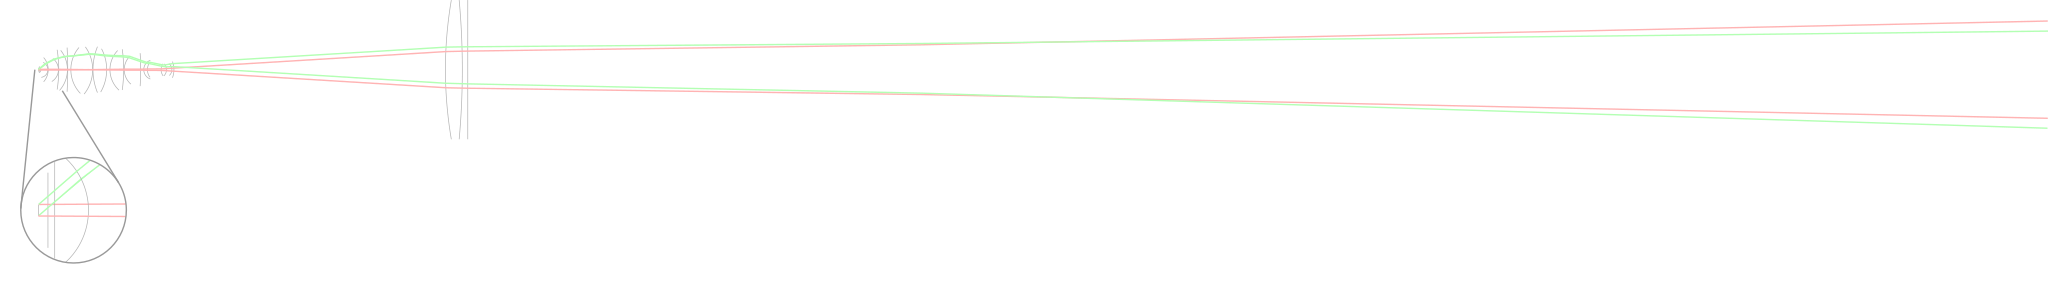
\includegraphics{objective-trace}



  \vspace{-5cm}
  
  \hspace{4cm}\textsf{\Huge Spatio--Angular Microscopy}
  
  \vspace{2cm}
  \hspace{6cm}\textsf{\huge PhD Thesis}


  \vspace{3cm}
  \hspace{4cm}\textsf{\Large Martin Kielhorn}
  
  \vspace{1cm}
  \hspace{4cm}\textsf{\Large July 10, 2012}
\end{titlepage}
\newpage
\section*{Abstract}
\begin{summary}
Photobleaching and phototoxicity pose a problem in live cell
imaging. Fluorescence imaging induces reactive oxygen species in
observed organisms which can alter the behaviour of the sample, and so
minimising light exposure is an important goal.

We augment a widefield epifluorescence microscope with two spatial
light modulators. By controlling the spatial illumination pattern and
the angle at which illumination occurs, we achieve control of the
illumination pattern in three dimensions.

Our custom software is used to obtain an initial image stack of the
specimen. Subsequent image sections are exposed with excitation
patterns that take into account the previous image stack. Depending on
the distribution of fluorophores this adaptive exposure can
considerably reduce photobleaching and phototoxicity.

We will use a protocol to characterise the phototoxic impact by
\todo{need to get results} imaging \emph{C. elegans} embryos and
counting the number of nuclei present after a given time.  This will
allow us to compare the performance with conventional spinning disk
and confocal microscopes and we will be able to quantify the
phototoxic impact of different microscopes and illumination
strategies.
\end{summary}

\urlstyle{sf}
%\setcounter{tocdepth}{3}
\section*{Preface}
\subsection*{Introduction}
\subsection*{Source Code Availability}
The source code is available on \url{https://github.com/plops/mma}.
It contains implementations for:
\begin{itemize}
\item illumination planning based on raytraces (see Appendix
  \ref{sec:raytrace})
\item moving the $z-$stage of a Zeiss Axiovert 200M microscope body
\item controlling an Andor Clara camera using the Andor SDK version
  2. For the following other cameras control software was written:
  \begin{itemize}
  \item Photometrics Cascade~II (interface to unsupported
    closed-source driver, only works on very old 32-bit Linux kernels)
  \item mvBlueFox 102G using the SDK
  \item Logitech Pro 9000 using a generic Video4Linux interface
  \item Andor sCMOS using Andor SDK version 3
  \end{itemize}
\item displaying patterns using a graphics card, that supports OpenGL,
  on a ForthDD SXGA ferroelectric LCoS display
\item controlling a standalone ForthDD WXGA 3DM display controller
  using USB
\item estimating the parameters of a rigid transformation between
  camera and LCoS display (see Appendix \ref{sec:rigid}),
\item controlling the micro-mirror array by Fraunhofer IPMS using
  their SDK
\item some specific image processing needs:
  \begin{itemize}
  \item three-dimensional convolution and Fourier transforms
  \item drawing of lines and ellipsoids in volumes
  \item rasterization of triangles (for creating shadow maps in the
    BFP, see section \ref{sec:trace-detect})
  \item calculation of optical transfer function for high NA
    objectives
  \item localization of in volumetric data \citep{Santella2010}
  \end{itemize}
\end{itemize}
The main development was done using GNU~Linux. However, portability
was kept in mind and most of the code will work in Microsoft Windows
as well.

\subsection*{Acknowledgements}
I would like to thank my supervisor Rainer Heintzmann, Kai Wicker,
Jakub Nedbal, Susan Cox, Daniel Appelt, Ond\v rej Mandula, Ronny
F\"orster, Ivana Sumanovac, Eckhard Birkner, Kathrin Klehs and all the
other members of our group for valuable discussions, support and
review of the manuscript.

I also thank Erhard Ipp, G\"unter Z\"ochling, Vincent Galy, QueeLim
Ch'ng, J\"org Heber, Mark Eckert, Dirk Berndt, Joel Seligson and
Jean-Yves Tinevez.  Thanks to the European Union Framework Programme 7
(project number 2115597) for the studentship on this project.  Further
I thank the Miroslav Grajcar, Edward Rosten, Christophe Rhodes, Paul
Khuong, Nikodemus Siivola, Levente M\'esz\'aros and Lu\' is Oliveira.

Finally I want to thank the authors and contributors to the following
free software projects: Linux, GCC, Emacs, SBCL, Maxima, Micromanager,
DIPimage, Wireshark, Latex, Inkscape, Gimp, ImageJ/Fiji and Blender.

\newpage
\tableofcontents
\printnomenclature
\newpage
\chapter{Introduction}
Fluorescence microscopy is an old technique that has been established
in live sciences for a long time. Being able to see things happening
at the micrometre scale is the fundamental path to understand life and
disease.

Innovation continuously improves microscopy and occasionally new
fields of research are opened up: The discovery and development of
fluorescent proteins initiated a revolution in how microscopy can be
applied in living specimen. Optical high resolution techniques allow
to observe biological processes at the scale of individual molecules
(tens of nm). 

Labels that report membrane potentials or viscosity within cells,
compounds that locally release chemicals when illuminated by light or
even ion pumps that can be switched by light promise novel interesting
research.

All these techniques have in common, that excitation light has to
reach a focal point, line or plane within the sample which consists of
a more or less dense fluorophore distribution.

With few exceptions (2-photon, SPIM, CLEM) microscopes are generally
not optimized for exciting only the in focus fluorophores.

Here we build a spatio-angular microscope. It contains two
programmable masks and can control which parts of the sample (spatial)
are illuminated by what angles. Its applications will mostly cover
imaging of living organisms experiments in them. There the effects of
phototoxicity are strongest and our microscope has an advantage over
conventional techniques.

\newpage
\newenvironment{fenster}{%
  \begin{addmargin*}[
  5em]{5em}%
    \begin{minipage}{\linewidth}%
    \vspace{1em}
      \rule{\linewidth}{2pt}%
}{%
    \rule[
.25\baselineskip]{\linewidth}{2pt}%
\vspace{1em}
    \end{minipage}%
  \end{addmargin*}%
}
\renewcommand{\H}{\textsf{H}}
\renewcommand{\O}{\textsf{O}}
% /mnt/backup/safe-with-time/torben/safed/y2009/0411
\section{Fundamentals of fluorescence}
\begin{summary}
  Here we give a short overview of the field of fluorescence of
  molecules in order to introduce the terms Stokes shift, triplet
  state and photobleaching.
\end{summary}
\subsection{Construction of molecular orbitals}
First we consider a very simple molecule: We move the nuclei of two
hydrogen atoms and move them slowly together. When the nuclei have a
big distance, the atoms exist as two separate entities without
influence on each other. In the other extreme case the two nuclei are
at the same position and the electrons have the orbitals of a helium
atom.
\begin{figure}[!hbt]
  \centering
  \input{flu-potential_my.eps_tex}
  \caption{Schematic electron density maps and potential curves for
    ground state $\H_2$ and excited state $\H_2^*$ of molecular
    hydrogen and the cation $\H_2^+$ of molecular hydrogen
    \citep[inspired from][p.~258]{Haken2006}.}
  \label{fig:flu-potential_my}
\end{figure}

For internuclear distances in between these two extremes, we express
molecular orbitals as a linear combination of atomic orbitals and
calculate their potential energy in dependence of the distance between
the nuclei (see \figref{fig:flu-potential_my}). The curve for
$\sigma_g\sigma_g^1\Sigma_g^+$ is minimal at a internuclear distance
$R$ of approximately 1.3 Bohr radii
($a_H=\unit[0.529\cdot10^{-8}]{cm}$). The compound of two protons and
two electrons is particularly stable for this distance. We call it the
hydrogen molecule $\H_2$.

Likewise a linear combination of the atomic orbitals of a ground state
hydrogen atom $\H$ with an excited hydrogen atom $\H^*$ lead to the
molecular orbital $\sigma_g\pi_u^1\Pi_u$. There, a minimum in the
potential occurs at an increased internuclear distance (bond
length). The excited atomic orbital has a reduced probability density
close to the nucleus but similar electron--electron
repulsion. Therefore the strength of the molecular bond (order of the
bond) is reduced.
\newcommand{\vmu}{\mbox{\boldmath{$\mu$}}}
\subsection{Absorption and emission of light}
A transition between a ground state $S_0$ to an excited state $S_1$
occurs, when a radiation field connects the two states. The connection
is described by the transition dipole moment
$\vmu_{0\rightarrow 1}$.
\begin{align}
  \vmu_{0\rightarrow 1} &= \int \psi^*_0 \vmu \psi_1 \textrm{d}^3V
\end{align}
where $\psi_0$ and $\psi_1$ are wavefunctions for the ground and
excited state, respectively \citep{Klessinger1989}.

An incident photon can electronically excite a molecule from the
highest occupied molecular orbital (HOMO), usually the singlet ground
state $S_0$, into the lowest unoccupied molecular orbital (LUMO), the
singlet excited state $S_1$.\nomenclature{HOMO}{highest occupied
  molecular orbital}\nomenclature{LUMO}{lowest unoccupied molecular
  orbital} For this, the energy $E_\textrm{ph}=hc/\lambda$ of the
photon has to match the energy gap $\Delta E=E_{S_1}-E_{S_0}$ of a
possible electronic transition within the molecule (Bohr's frequency
condition).

Photons with wavelengths below \unit[200]{nm} have sufficient energy
to ionize molecules. On the other side of the spectrum, a dye that
absorbs in the near-infrared ($\unit[>700]{nm}$) has a low-lying
excited singlet state $S_1$ and potentially increased reactivity
\citep{Sauer2011}. Hence, most known stable and bright fluorophores
absorb and emit in the wavelength range between \unit[300]{nm} and
\unit[700]{nm}.

As opposed to atomic spectra the absorption bands of organic dyes
usually span several tens of nanometers\footnote{Note that wavelength
  isn't a convenient unit to characterize absorption bands. Rather one
  should use energy or wavenumbers.}. This is because dye molecules
are composed of many atoms and this structure can vibrate, rotate and
interact with the solvent.
\subsection{Vibration of molecules}
The distance between the two nuclei of the hydrogen molecule is not
rigid. The nuclei can oscillate around their position of equilibrium
at quantized frequencies. The vibration frequencies depend on the
order of the bond and the mass of the two nuclei. When a molecule is
electronically excited, its vibration frequencies decrease.
\begin{figure}[!hbt]
  \centering
  % (423-120)/423*7 = 4.77 ,trim=0 0 135 0,clip
  \input{flu-condon_my.eps_tex}
  \caption{Illustration of the Franck-Condon principle. Potential
    curves for either the same bond length in the
    excited state ({\bf left}) or a larger bond length in the
    excited state ({\bf right}). Electronic transition occurs
    instantaneously and excites higher vibro-rotational states in the
    right diagram. \citep[inspired from][p.~276]{Haken2006}.}
  \label{fig:flu-condon}
\end{figure}

\figref{fig:flu-condon} schematically shows potential curves for the
ground state $S_0$ and the first excited state $S_1$ of two different
molecules. The left graph depicts a molecule where the internuclear
distance is the same in the ground $S_0$ and excited $S_1$ stage. When
such a molecule absorbs a photon, its electron is excited but its
vibrational mode does not change. The anthracene molecule shows such
behaviour.

The right graph depicts a molecule that has a larger internuclear
distance in its excited state. When a photon is absorbed, the
electronic state of the molecule transitions into the higher state
$S_1$. The mass of the electron is much smaller than the
nucleus. Therefore the electronic transition takes place in a
timescale of $\unit[\sim10^{-15}]{s}$. In this duration the nuclei do
not move (\emph{Born-Oppenheimer approximation}: electronic
transitions occur as if the nuclei were fixed in place). The changed
bond length with the new orbital of the excited state $S_1$ drives the
nuclei into movement (excitation of vibro-rotational modes,
\emph{Franck-Condon principle}: electronic transition most likely
occurs without changes to the position of the nuclei and the intensity
of a vibrational transition depends on the overlap between the
vibrational wavefunctions).

\subsection{Depopulation pathways of excited states}
\begin{figure}[!hbt]
  \centering
  \def\svgscale{.8}
  {\small
  \input{flu-level_my.eps_tex}}
  \caption{A typical energy level diagram. The boxes depict orbitals,
    up and down arrows symbolize the spin of the outer electrons. Fat
    lines represent electronic states. Thinner lines indicate
    vibro-rotational states. Various processes are shown with their
    typical time scales. VR = vibro-rotational relaxation, ISC =
    intersystem crossing, IC = internal conversion \cite[inspired
    from][]{Haken2006}.}
  \label{fig:flu-level}
\end{figure}
The Jablonski diagram in \figref{fig:flu-level} summarizes information
about the energy levels of a molecule and possible transition
processes. If a molecule is in the ground state $S_0$ one of its outer
electrons can be excited by absorbing a photon to the first excited
singlet state $S_1$.  If the photon has an even higher energy, the
electron will go into the second excited singlet state $S_2$.

Transition from the ground state into higher electronic states than
$S_2$ is not usual in commonly used fluorophores and wavelength range.
Absorption of one photon doesn't change the spin of an electron and
therefore the transition $S_0\rightarrow T_1$ into the triplet state
$T_1$ only occurs with very low probability.

\subsubsection{Kasha's rule}
As described above, electronic excitation in general also leads to the
excitation of a vibro-rotational nonequilibrium state (Franck-Condon
state). In microscopy, fluorophores are often in solution, where they
experience at least $10^{12}$ collisions per second. Inter- and
intramolecular interactions bring the vibrations of the fluorophore
molecule back to thermal equilibrium\footnote{Rotation states have
  energies corresponding up to \unit[100]{$cm^{-1}$} (microwave),
  vibration states have energies corresponding to wavenumbers from 300
  to \unit[3000]{$cm^{-1}$} (infrared). Electronic states have
  energies in the visible. The number of excited molecules in thermal
  equilibrium is governed by the Boltzmann law and proportional to
  $\exp(-\Delta E/(k_BT))$. Therefore, at room temperature ($k_B
  T\sim\unit[200]{cm^{-1}}$), only rotation states are excited. } in a
very short timescale ($\unit[10^{-12}]{s}$). This is considerably less
then the lifetime of the electronic excitation (few
nanoseconds). Therefore spontaneous emission of a photon will occur
from the vibrational ground state $S_{1,v_1=0}$ (\emph{Kasha's rule}).

\subsubsection{Stokes shift}
During emission of a fluorescence photon a Franck-Condon state of the
singlet ground state $S_0$ is excited and returns into thermal
equilibrium by vibro-rotational relaxation. Thus, some of the energy
of the original excitation photon is lost as heat. The emitted
fluorescence photon is red shifted compared to the excitation
photon. Technically the \emph{Stokes shift} is defined as the
difference of the wavenumbers of the fluorescence maximum and
absorption maximum\footnote{Sometimes the Stokes shift is also defined
  as the distance of the absorption maximum to the point where the
  normalized absorption and emission curves intersect.}.

In terms of wavelength the Stokes shift usually corresponds a change
of 15 to \unit[30]{nm}. The Stokes shift is bigger, when the shape and
position of the potential of the excited state $S_1$ differs from the
ground state $S1$ (see \figref{fig:flu-condon}, right). There are
fluorophores with more than \unit[100]{nm} Stokes shift.

\subsubsection{Internal conversion}
Often the transition $S_2\rightarrow S_1$ occurs by \emph{internal
  conversion} (IC) followed by vibro-rotational relaxation. During IC,
the electronic state transitions into a high vibro-rotational
excitation of a lower electronic state. The probability for IC is high
for a high density of vibrational target states.
% FIXME translate Zustandsdichte

For floppy, non-rigid molecules, IC is a competing process to
fluorescence $S_1\rightarrow S_0$. In dyes that absorb in the near
infrared, the energy gap between $S_0$ and $S_1$ is so small and the
vibrational states of highest energy of the singlet ground state $S_0$
(vibration of hydrogen bonds directly attached to the chromophore) are
close to $S_1$. This seriously reduces the efficiency of infrared dyes
\citep[p.~43]{Sauer2011}.


\subsubsection{Fluorescence quantum yield}
The \emph{fluorescence quantum yield} $\eta$ of a fluorophore is
defined as the quotient of the number of emitted (fluorescence)
photons and the number of absorbed photons. In dyes like rhodamine~6G
(in ethanol $\eta=0.94$ \cite{Fischer1996}) or anthracene
(9,10-diphenyl anthracene in cyclohexane $\eta=0.90$ \cite{Hamai1983})
its value can be nearly 1 in an appropriate solvent.


\subsubsection{Intersystem crossing}
There is a small probability that the HOMO electron doesn't relax by
internal conversion or emission of a fluorescence photon. Instead it
flips its spin (due to spin-orbit coupling\footnote{The probability of
  a spin flip is increased if heavier atoms are part of the
  molecule. E.g.\ while fluorescein has a triplet yield of 0.03, the
  triplet yield of eosin, a fluorescein derivative with four bromine
  substituents is 0.76 \citep[p.~37]{Sauer2011}.}). This process is
called \emph{intersystem crossing} and populates the first triplet
state $T_1$. A transition into the ground state $S_0$ would need
another spin-flip of the electron and is quite improbable. Therefore
the triplet state has a long lifetime (up to several seconds). The
radiative decay is called phosphorescence.
  

\subsection{Photobleaching and phototoxicity}
The prolonged lifetime of the triplet state $T_1$ increases the
probability for the excited molecule to collide with a partner and
react.

\begin{figure}[!hbt]
  \centering
  \input{oxygen.eps_tex}
  \caption{{\bf left:} Molecular orbitals of the oxygen molecule. {\bf
      right:} Molecular oxygen has the lowest energy in its triplet
    state ${}^3\Sigma$. Then the spins of the two $\pi^*-$electrons
    are parallel. Inspired from \citet{Linde2011a}.}
  \label{fig:oxygen}
\end{figure}


The ground state of the oxygen molecule is a triplet state ${}^3\O_2$,
with two unpaired electrons of parallel spin in its $\pi^*-$orbitals
(see \figref{fig:oxygen}). The triplet ground state and its abundance
in typical microscope samples are the reasons why oxygen is so
important when it comes to phototoxicity. If an oxygen molecule comes
into physical contact with a $T_1$ fluorophore, e.g.\
${}^3\textsf{Chlorophyll}^*$, the energy of the dye can be transferred
to the oxygen by an electron exchange energy transfer mechanism in
which the orbitals directly interact with each other
\citetext{\citealp[p.~438]{Haken2006} and \citealp{Linde2011a}}:
\begin{align}
  {}^3\O_2 + {}^3\textsf{Chlorophyll}^* \rightarrow
  {}^1\O^*_2+{}^1\textsf{Chlorophyll}
\end{align}
This reaction is also known as triplet--triplet annihilation.  There
are two forms of singlet oxygen, that form in competition: The lower
energy ${}^1\Delta$ and the short-lived, higher energy ${}^1\Sigma$
form ($T_{1/2}\sim\unit[10^{-9}]{s}$), with spin orientations as
depicted on the right of \figref{fig:oxygen}. During the transition
${}^1\Sigma\rightarrow{}^1\Delta$ an infra-red photon with
\unit[1268]{nm} wavelength is emitted \citep[p.~20]{Linde2011a}.

The resulting singlet oxygen is very reactive and when it reacts with
the fluorophore, it can destroy it (photobleaching) also the singlet
oxygen is quite hazardous inside living creatures. Plants have
developed several protection mechanisms against being exposed to too
much light. Within the cells they reorient and shift their
chloroplasts in order to expose them to less light \citetext{priv.\
  comm.\ V. Sarafis}. % Today I heard, that he died.
However, they even have a molecular protection
mechanism: They transfer the energy of the chlorophyll onto carotenoid
molecules and can prevent the hazardous \emph{phototoxicity} effects
of singlet oxygen \citep{Krieger-Liszkay2005}.

Nowadays many methods are known to reduce photobleaching. Supplant
oxygen with noble gases or remove it enzymatically
\citep[p.~89]{Sauer2011}. Depopulate the triplet state by adding
reducing as well as oxidizing agents to the solvent
\citep{Vogelsang2008} or couple a triplet quencher directly to the
fluorophore \citep[p.~19]{Sauer2011}. For fixed samples it helps to
change the solvent or polymer.

All these techniques work after the hazardous chemicals have been
produced. In order to reduce phototoxicity even more it makes sense to
think about the light management in the microscope. 
\section{Conventional microscopes}
\begin{summary}
  Microscopes that are in common use today do not optimally excite
  fluorophores within the specimen. In this section we outline how
  these microscopes work. We explain how out-of-focus blur severely
  limits the performance of the wide field microscope. Then we discuss
  how confocal microscopy improves the sectioning capability at the
  cost of increasing the phototoxic load on the specimen.
\end{summary}
The basic building block of microscopes are lenses. A lens is a piece
of glass with two polished spherical surfaces. Aspherical lenses also
exist but are much harder to manufacture because of their lower
symmetry. Light is slower in glass than in air. The shape of a lens
redirects photons and the thickness of the material can delay them. A
lens ideally focuses a parallel beam of light into a spot on its focal
plane. The distance between focal plane and the region where the rays
start to converge is called focal length and denoted by $f$.
\begin{figure}[!hbt]
  \centering
  \input{widefield-microscope.eps_tex}
  \caption{{\bf a)} Schematic of a modern microscope. The sample is in
    the front focal plane of the objective. The detection tube lens TL1
    forms a magnified image on the camera. {\bf b)} Wide field
    epifluorescence excitation. The excitation tube lens focuses a
    laser into the back focal plane (BFP). The beam is reflected by a
    dichroitic beam splitter (BS) towards the objective. An extended
    area in the specimen is illuminated. Fluorescence light of lower
    wavelength returns through the objective, is transmitted through
    BS and forms an image on the camera. {\bf c)} Confocal
    microscope. A pinhole PH2 is imaged as a diffraction limited spot
    into the specimen. Returning fluorescence light is only detected
    when it passes through an aligned pinhole PH1. This configuration
    rejects light that doesn't originate from the front focal plane
    (green) of the objective.}
  \label{fig:widefield-microscope}
\end{figure}

The uncoloured beam in \figref{fig:widefield-microscope}~a) represents
rays that start from the intersection $O$ of the optical axis and the
front focal plane of the objective. The objective collects the rays
and collimates them into a beam that is parallel to the optical
axis. After traversing the tube length $f+f_\textrm{TL}$, the rays are
focused by the detection tube lens TL1 on the intersection $O'$ of its
focal plane and the optical axis. 

The blue beam corresponds to rays that start from an off-axis point
$P$ in the front focal plane of the objective. Behind the objective
the blue beam is a parallel beam. However, the beam is tilted relative
to the optical axis. The tube lens TL1 focuses the blue beam into a
spot at $P'$ on its focal plane.

The objective fulfils the Abbe sine condition -- it is aplanatic. The
microscope forms stigmatic images of points from the front focal plane
in the plane perpendicular to the optical axis, containing $O'$ and
$P'$. The plane with the images is called intermediate image plane. It
is magnified by the factor $M$:
\begin{align}
  M=\frac{\overline{O'P'}}{\overline{OP}}=\frac{f_\textrm{TL}}{f}.
\end{align}
In our microscope we use an objective with magnification $M=63$. The
focal length of the tube lens is \unit[164.5]{mm} for most Zeiss
microscopes. Therefore the focal length of our objective is
$f=\unit[2.61]{mm}$.

Let's assume we have an opaque sample with just two small
($\diameter<\unit[120]{nm}$) holes with $\unit[2]{\mu m}$ distance
between them.  We put this object into the front focal plane of the
objective and position a camera on $O'$. When illuminating the mirror
from the side opposite to the objective, the camera will show two
spots with $\unit[126]{\mu m}$ distance.

\nomenclature{NA}{numerical aperture}

Note that \figref{fig:widefield-microscope} depicts a \emph{thin-lens
  model of a high numerical aperture objective} that fulfils Abbe's
sine condition. A real objective contains in the order of ten coated
lenses of different glass and crystalline materials. Their curvatures,
positions and materials were all carefully chosen, taking into account
manufacturing tolerances and wavelengths, so that the microscope
behaves as the thin-lens model predicts. Diffraction at the periphery
of the pupil in the back focal plane dictates the resolution, one can
achieve inside of the sample.

It is quite possible that heating to \unit[37]{${}^\circ$C} will ruin
such a high-precision instrument. A related source of aberrations
(departure of design performance) is the refractive index inside of
the specimen. In Appendix~\ref{sec:ray-aberration} we describe a more
complicated model that can predict the effect of embedding the sample
in water (instead of immersion oil with the same refractive index as
the glass).

\subsection{Widefield epifluorescence microscope}
Fluorescence photons are emitted in all directions, independent of the
original illumination direction. Therefore it is possible and
convenient to use the objective for excitation as well as
detection. This mode of microscopy is called epifluorescence (Greek:
$\varepsilon\pi\iota$; on, above).  In this configuration usually only
a small percentage of the excitation light returns due to diffraction
or reflection. This simplifies the separation of fluorescence light
from excitation light.  Furthermore parts of opaque specimen can be
imaged and it is beneficial that the illumination needs to be aligned
only once.

\nomenclature{BFP}{Back focal plane}

The red beam in \figref{fig:widefield-microscope}~b) is a parallel
laser. The excitation tube lens TL2 focuses the beam into the back
focal plane (BFP) of the objective. The beam is reflected at a
dichroitic beam splitter (BS). This is a glass plate that has been
coated with dielectric layers. The refractive index, thickness and
sequence of the layers are designed so that the excitation light is
reflected towards the objective but lower energy fluorescence light
returning from the objective is transmitted towards the camera. Behind
the objective the beam is parallel and illuminates the specimen. The
\emph{field of view} is the demagnified diameter of the laser beam
before TL2.
\subsubsection*{Non-uniformity due to coherent interference}
Note that tiny dirt particles and coherent interference in laser beams
can produce unwanted non-uniformities in the illumination. As a remedy
the spatial coherence of the laser is sometimes reduced.  Incoherent
light emitting diodes, mercury or xenon arc lamps are often used
instead of lasers. In the latter case a band pass filter selects the
useful part of the spectrum of the excitation lamp upstream of the
dichroitic beam splitter.

\subsubsection{Out-of-focus blur}
However, independent of the choice of the light source, the wide field
microscope in epifluorescence configuration exposes many layers of the
sample. This leads to fluorescence of out-of-focus fluorophores.

There are two reasons, why out-of-focus fluorophores give blurred
images. Not even an ideal imaging system -- a device that forms
%% FIXME refer to maxwell or born/wolf
stigmatic images of all the points in one volume in another volume --
would form sharp images on the camera plane. After all, the camera is
just a plane and the object under observation is three dimensional.

Furthermore a microscope is far from being an ideal imaging system. In
a microscope it is not possible to obtain a sharp image of a different
slice of the object by changing the axial position of the camera
behind the tube lens TL1 \citep{Botcherby2007,Botcherby2008a}.
\subsubsection*{Deconvolution}
When a stack of several slices of an object is obtained, it is
possible to suppress the blurred part of each image in all the
others. These algorithms (deconvolution) can improve the perceived
quality of images in some stacks. However, there are two fundamental
problems:

First the \emph{missing cone problem} prevents focusing on a
homogeneous fluorescent plane. Physics dictates that there is always a
gap in the transfer function of the objective when the fluorescence
process is linear and the objective collects only photons from one
half space (see \figref{fig:missing-cone}). Not all spatial
frequencies within the transfer function attenuate with defocus
\citep{Neil1997}.

\begin{figure}[!hbt]
  \centering
  \input{missing-cone.eps_tex}
  \caption{Schematic to depicting $k_xk_z-$cross sections of the
    support of optical transfer function (see
    Appendix~\ref{sec:app_hilo}) for microscope objectives with
    different collection angles. {\bf left \& middle:} Objectives,
    that only collect one light that is directed into one half space,
    have the missing cone problem. There, low spatial frequencies
    don't attenuate with defocus. {\bf right:} Theoretical objective
    with larger collection angle and no missing cone.}
  \label{fig:missing-cone}
\end{figure}

Second, even with ideal detectors there is photon shot noise in the
image. In deconvolution algorithms the image of one slice is improved
by subtracting blurred versions of the other slices. When the blurred
intensity is large, its shot noise is high as well. Subtraction only
increases noise and a faint in-focus image can be severely
deteriorated by the noise of the out-of-focus light.
\subsection{Confocal microscope}
One way of addressing both problems of the wide field microscope is
depicted in \figref{fig:widefield-microscope}~c). In the confocal
microscope the whole field of view isn't illuminated simultaneously.
The excitation tube lens TL2 collimates the light coming from a
pinhole PH2 and illuminates the full back focal plane of the
objective. In the front focal plane of the objective the red beam then
converges to illuminate the smallest possible single spot. The spot
size is defined by diffraction at periphery of the BFP. However,
out-of-focus fluorophores are still being excited by the hour-glass
shaped illumination.

The eponymous idea of the confocal microscope is to replace the camera
with a pinhole PH1. This pinhole hardly affects the light detected
from in-focus fluorophores. However, an out-of-focus fluorophore that
is defocused by $\Delta z$ towards the objective will lead to a
diverging beam (colorless) at the tube lens and will be imaged into a
point behind the focal plane of the tube lens. The pinhole only
transmits a part of the circle of confusion. Hence defocused
fluorophores contribute less to the sensor signal.

An image of the in-focus specimen is obtained by scanning the pinholes
over the field of view and measuring intensity at each position
individually. The optical removal of out-of-focus light prevents
degradation of the signal by its shot noise and improves the
point-spread function of the objective. The missing cone problem is
fixed and the transversal resolution improved by a factor of $\sqrt
2$. Note however, that information about out-of-focus fluorophores is
lost which would be obtained in a wide field microscope with
deconvolution. Therefore a wide field microscope will give better
results when a lot is known about the sample structure and this
knowledge is fed into the deconvolution. E.g.\ the localization of
sparse beads of specific size will be better in a wide field
microscope.

The confocal microscope was invented in 1955 \todo{check patent
  citation} \citep{Minsky1961,Minsky1988} to reduce the influence of
scattering effects in neuron samples stained by Golgi's method. This
invention preceded the laser and was unfortunately not put into
practical use for biology until three decades later \citep{Amos1987}.
\subsection{Phototoxicity in conventional microscopes}
When imaging living specimen we should distinguish between useful and
unnecessary excitation. Taking into account the detection capabilities
of objective lenses we should maximize the ratio of in-focus to
out-of-focus fluorescence. The epifluorescent wide field and confocal
microscope surely do not represent an optimum in this regard.

The following chapter \ref{sec:approaches} will introduce other
microscopy techniques that are more considerate of where to deposit
excitation power within the specimen.
\subsection{2-photon laser scanning fluorescence microscopy}
If an intense subpicosecond pulse of infrared light is focused into a
spot in the sample, non-linear 2-photon absorption can occur
\citep{Denk1990}. Infrared light is scattered less than visible light
of half the wavelength. For similar excitation rates, the
phototoxicity in the focus is higher than in a single-photon
microscope. However, there is no excitation in the out-of-focus
region. Therefore a detection pin hole is not required.

This technique has greatly improved depth of penetration and
sensitivity of in situ imaging
\citep{Otsu2008}. % sentence from otsu 2008
\section{Image detectors in wide field microscopy}
\label{sec:ccd-intro}
\begin{summary}
  Here we describe CCD\nomenclature{CCD}{charge-coupled devices}
  sensors and their characteristics.
\end{summary}
Charge-coupled devices are semiconductor devices that contain a 2D
grid of capacitors, formed by at least three groups of electrodes
(phases). Cycling the voltage on these electrodes allows to push
charges, which has been accumulated under the capacitors (registers)
into their neighbours. They turned out to be the ideal tool to move
charges, produced by photon absorption in light sensitive diodes,
across the substrate into read out logic.

Forty years of development lead to imaging devices with remarkable
charge transfer efficiency, high quantum efficiency (up to 95\% with
back illumination) and very low dark currents. Until ten years ago the
performance of CCD imagers in the low light regime was limited by the
noise of the read out amplifier (a few electrons per pixel
rms\footnote{root mean square} \todo{rms}).

Now we have electron multiplying CCD (EM-CCD)
\nomenclature{EM-CCD}{Electron multiplying charge-coupled devices
  (p. \pageref{sec:ccd-intro}, \pageref{sec:ccd-meas})} technology,
which allows comparably good performance at low photon numbers
\citep{Mackay,Robbins2003} and moderate read out speeds (tens of
MHz). EM-CCDs contain a row of additional registers in front of the
read out circuit. There, one of the three phases is clocked with a
much higher voltage (up to \unit[40]{V}) then is needed purely for
charge transfer ($\unit[\sim6]{V}$). The large electric fields cause
charge carriers to be accelerated to sufficiently high velocities, so
that additional carriers are generated by impact ionization. The
charge multiplication per transfer is small ($\sim1\%$) but by using
several hundred registers a substantial gain in the number of charges
can be achieved. In microscopy we usually work with gains of up to
300. Higher gains are possible but limit the dynamic range.

The charge amplification helps to push the read noise from
$\sim\unit[40]{electrons\ rms}$ to significantly below
$\unit[1]{electron\ rms}$ --- in effect creating a sensor limited only
by the photon noise. However, the multiplicative nature of the gain
leads to a perceived reduction in the quantum efficiency of the sensor
(excess noise factor), i.e. an image with $\unit[100]{photons/pixel}$
without gain will look like the same image at only
$\unit[50]{photons/pixel}$ with EM-gain (see Appendix
\ref{sec:ccd-meas}).


\chapter{Other approaches of light control}
\label{sec:approaches}
\nomenclature{CLEM}{Controlled light exposure microscopy}%
\begin{summary}
  This chapter gives an overview of current microscopy techniques that
  reduce unnecessary fluorescence excitation and reduce
  phototoxicity. In \emph{light sheet microscopy}, an oblique sheet of
  light illuminates the sample without exposing too many out-of-focus
  fluorophores. \emph{Controlled light exposure microscopy} (CLEM)
  takes into account the in-focus fluorophore distribution and
  iteratively improves the signal-to-noise ratio of the measurement.
  Finally, \emph{light field microscopy} allows instantaneous and
  complete control of all parameters of the incoherent light exposure.
\end{summary}
\section{Light sheet fluorescence microscopy}
\begin{summary}
  Light sheets can be directly created with separate optics to
  illuminate the sample from an orthogonal direction. Another
  promising method to create a sheet is to use a high numerical
  aperture objective near the total internal reflection
  angle. Diffraction couples the minimum width of the sheet and the
  extent of the area, where the sheet's width is constant. There is a
  trade-off between sheet width and field of view.
\end{summary}
The idea of illuminating a sample from the side dates back quite far
into the history of microscopy. Already one hundred years ago, an
objective perpendicular to the detection objective was used for
illumination of the focal plane in the specimen. This dark field
technique was used to characterize gold nano particles in gold ruby
glass \citep{Siedentopf1903}.

Eventually this technique was applied to fluorescence
microscopy. First to analyze cochlea specimen \citep{Voie1993} and
more recently for the development of embryos
\citep{Huisken2004}. Results in the latter paper have sparked interest
in the technique at many labs \citep{Santi2011}.
\subsection{Light sheet generation with cylindrical lens}
\begin{figure}[!hbt]
  \centering
  %\bild{spim}
  \input{spim-sketch.eps_tex}
  \caption{Schematic of SPIM (selective plane illumination
    microscopy). A cylindrical lens illuminates the specimen with a
    thin sheet of light along the focal plane of the
    objective. Rotating the sample and/or moving it along the axis
    allows to reconstruct a sectioned three-dimensional volume of the
    fluorophore concentration with improved light utilization compared
    to conventional microscopes \citep[inspired from][]{Huisken2004}.}
  \label{fig:spim}
\end{figure}
\figref{fig:spim} shows how the light sheet can be focused into the
specimen using a cylindrical lens. \cite{Huisken2004} employ a water
dipping objective with long working distance (\unit[1\ldots 2]{mm})
and comparatively low NA for detection. A $10\times$ objective with
$\unit[660]{\mu m}$ field of view diameter is used with a sheet that
varies less than $42\%$ in thickness ($\unit[6\ldots 8]{\mu m}$). The
light sheet not only improves sectioning and contrast but also
improves the axial resolution from originally $\unit[14]{\mu m}$ by
nearly a factor of two.

\nomenclature{SPIM}{Selective plane illumination microscopy}

The axial resolution of detection objectives of higher numerical
aperture isn't improved so easily over an extended field of
view. Shading effects, diffraction and refraction can deteriorate the
light sheet. As an improvement of the technique it was suggested to
rotate the specimen or illuminate with multiple sheets of light from
different directions.

Other improvements involve a Bessel beam that is scanned to illuminate
a plane. This intensity distribution is ``self-reconstructing'' and
can compensate better for obstacles in its path. It comes with the
cost that the light sheet isn't as confined. Simultaneous structured
illumination and 2-photon effects were suggested to improve this.


\subsection{Light sheet generation using the detection objective}
\label{sec:hilo}
\begin{figure}[!hbt]
  \centering
  \bild{dunsby}
  \caption{Schematic of oblique plane microscopy (OPM). An index
    matched sample is excited using an oblique plane of light. The
    illuminated plane is tilted relative to the focal plane. Therefore
    out-of-focus fluorophores on the periphery of the field of view
    are excited. Two additional objectives in the detection path are
    used to reconstruct an aberration free image of all the excited
    fluorophores (drawing from \cite{Dunsby2008}).}
  \label{fig:dunsby}
\end{figure}
Modern high numerical aperture objectives allow to illuminate an
\emph{index matched} sample with a half angle of up to
$70^\circ$. This enables illumination of an oblique and thin sheet of
light in the sample just as in selective plane illumination
microscopy. However this technique (oblique plane microscopy, OPM) has
the advantage, that only one objective is needed in order to be close
to the sample and it will work with specimen in conventional
microscope slides. However, one difficulty is that the excited
fluorophores are severely defocused in the intermediate image plane
(see \figref{fig:dunsby}). Dunsby describes how to rotate the
observational plane optically in order to recover an aplanatic image
from the oblique illumination plane \citep{Dunsby2008}. They re-image
the sample through two additional objectives.

\nomenclature{OPM}{Oblique plane microscopy}

\begin{figure}[!hbt]
  \centering
  \input{hilo-sketch.eps_tex}
  \caption{Schematic of rays in HILO (highly inclined and laminated
    optical sheet) technique. The specimen is embedded in a medium of
    lower optical density than the cover slip. For a very high
    illumination angle (point on the periphery of the back focal
    plane), the light would be reflected at the cover slip-medium
    interface due to total internal reflection. For HILO, a point on
    the back focal plane that is closer to the optic axis is
    illuminated. The light enters the embedding medium at a highly
    inclined angle and only a thin sheet in the focal plane is
    illuminated \citep[inspired from][]{Tokunaga2008}.}
  \label{fig:hilo}
\end{figure}

Biological specimen are often not index matched and have a lower index
$n_e\approx 1.33\ldots1.45$ than the immersion oil $n=1.52$. As
indicated in \figref{fig:hilo}, the refraction at the interface
between cover slip glass and embedding medium can be exploited to
illuminate the specimen with a light sheet that is nearly parallel to
the focal plane.  This technique is called highly inclined and
laminated optical sheet microscopy (HILO) \citep{Tokunaga2008,
  Konopka2008}.

\nomenclature{HILO}{Highly inclined and laminated optical sheet microscopy}

Note that the index mismatch between embedding and immersion medium
will introduce aberrations (mostly spherical) which will limit the
imaging depth.
\section{Scanning techniques for improving light utilization}
\subsection{Controlled light exposure microscopy (CLEM)}
\label{sec:CLEM}
The confocal microscope (see \figref{fig:widefield-microscope}~c)
allows another adaptive illumination technique. Each slice of a
specimen is partitioned into three different regions: areas with no
fluorophores (A), high concentration of fluorophores (C) or an
intermediate (B).

Ideally, the areas (A) that don't contain fluorophores should only be
exposed until fluorophore content is ruled out. The other two classes
(B) and (C) should be exposed until the same number of fluorescence
photons have been detected. This would result in an image with
constant signal-to-noise ratio. Unfortunately due to the photon nature
of light, sometimes a region of type (B) is incorrectly treated as A
which introduces dark pixel artifacts in the image
\citep{Hoebe2010}\todo{read reference}.

In conventional microscopes, areas of class (C) with high fluorophore
concentration are generally exposed too much. Their signal-to-noise
ratio would be high, but this doesn't increase the perceived image
quality. Furthermore, the regions above and below the focal plane are
unnecessarily subjected to high exposure.

The CLEM approach was first presented by Hoebe et al.\ in
2007,\todo{was that first, get}\ followed by an independent similar
version with adaptive control of the laser power for 2-photon
microscopy by Chu et al.\ \citep{Hoebe2007,Chu2007}.
\subsection{Acousto-optic deflectors for fast beam steering}
In a conventional confocal microscope, the beam is steered by two
galvanometer mirrors. This technique offers very good light throughput
and is sufficient to obtain rectangular images. However, the inertia
of the mirrors severely limit the access rate of spots in the focal
plane.

Replacing the mechanical mirrors with an acoustic wave in a
transparent material (TeO$_2$) enables $\unit[4]{\mu s}$ switching
time \citep{Otsu2008} and even allows re-focusing
\citep{Reddy2008}. These acousto-optic deflectors have lower
efficiency than mirrors (70\% for two AODs) and show chromatic
aberrations.

However, as descanning isn't necessary in 2-photon microscopy, the
lower efficiency (in the excitation path) is hardly an
issue. Therefore, this technique for the first time enables ``random
access'' of three-dimensional coordinates in the sample.

\begin{figure}[!hbt]
  \centering
  \bild{aod} 
  \caption{Schematic of an acousto-optic deflector (AOD) illumination
    system with $z-$focusing. Figure taken from \citet{Reddy2008}}
% in focusing single s highly preferred http://www.future-perfect.co.uk/grammartips/grammar-tip-focussed-focused.asp
  \label{fig:aod}
\end{figure}


\nomenclature{AOD}{Acousto-optic deflector}
\nomenclature{AOM}{Acousto-optic modulator}
\section{Non-scanning techniques}
\subsection{Direct illumination}
An obvious method for doing spatial control is to image a
two-dimensional array of high-power micro-LEDs into the specimen.
\begin{figure}[!hbt]
  \centering
  \includegraphics[width=7cm]{led-array} 
  \caption{An overlay combining wide field micro-LED illumination and
    fluorescence imaging YFP tag expressed in neurons, taken from
    \citet{grossman2010}.}
  \label{fig:led-array}
\end{figure}
However, the problem is to achieve sufficient \emph{irradiance} and
\emph{fill factor}. The angular emission profile of LEDs is often
Lambertian, i.e.\ the back focal plane of the objective would be
over-illuminated and a lot of light would be lost. The fill factor is
limited because it is difficult to put a lot of LEDs close to each
other.  The technique has been demonstrated using a $64\times64$ array
of $\unit[20]{\mu m}$ micro-emitters with $\unit[50]{\mu m}$ pitch
\citep{grossman2010}.  The LEDs can be switched at millisecond speed
and emit at $\unit[(470\pm22)]{nm}$.

\nomenclature{GFP}{Green fluorescent protein}
\nomenclature{EGFP}{Enhanced green fluorescent protein}
\nomenclature{YFP}{Yellow fluorescent protein}
\nomenclature{VCSEL}{Vertical-cavity surface-emitting laser}
\nomenclature{LED}{Light-emitting diode}
\nomenclature{MMA}{micro-mirror array}
\nomenclature{LCoS}{Liquid crystal on silicon (display)}
\nomenclature{DPSS}{Diode-pumped solid-state (laser)}

LED arrays enable interesting experiments where processes are
influenced by light, i.e.\ optogenetics, but the targets ideally have
to be located in the focal plane. Also, it must be verified that the
illumination cone of each LED image doesn't affect the measurement,
i.e.\ activate the specimen in the out-of-focus regions.

Nevertheless, once the LED or VCSEL arrays become available in
interesting spectral ranges, we might see the direct illumination
techniques more often.

\subsection{Intensity modulation}
\subsubsection{Programmable array microscopy}
A technique similar to controlled light exposure microscopy (CLEM,
section \ref{sec:CLEM}) has been implemented in a programmable array
microscope (PAM) \citep{Caarls2011}. Like our microscope, the PAM
images a pattern into the sample using a spatial light modulator. In
addition to our system, the same SLM is used in the detection path to
recover an image of the in-focus fluorophores.

\begin{figure}[!hbt]
  \centering
  \input{pam-sketch.eps_tex}
  \caption{Schematic of a programmable array microscope (PAM)
    \citep[inspired from][]{Verveer1998}. A digital micro mirror
    device (DMD) containing an array of tiltable mirrors is imaged
    into the focal plane of the objective. Returning fluorescent light
    from out-of-focus fluorophores is distributed onto both the
    cameras. In-focus fluorescence is only imaged onto camera 1.}
  \label{fig:pam-sketch}
\end{figure}


\nomenclature{PAM}{Programmable array microscopy}%
\nomenclature{DMD}{Digital micro mirror device}%
\nomenclature{MLE-PAM}{Minimized light exposure programmable array microscope}%

\subsubsection{Light field microscopy}
Interesting work on light fields originally started in the macroscopic
domain of cameras \citep{Lippmann1908%,Sokolov1911
} and was eventually applied as a technique for microscopy
\citep{Levoy2006,Levoy2009,Zhang2009}. This approach is built on
imaging through an array of microlenses.
\begin{figure}[!hbt]
  \centering
  %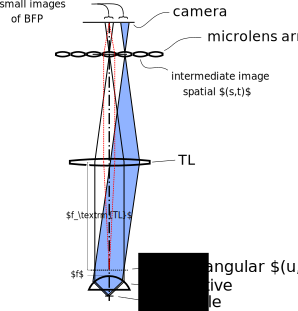
\includegraphics[width=7cm]{microlens-levoy-sketch} %FIXME redraw
  \input{microlens-levoy-sketch.eps_tex}
  \caption{Schematic of microlenses in intermediate image plane
    \citep[inspired from][]{Levoy2006}}
  \label{fig:microlens-levoy-sketch}
\end{figure}

A microlens array is placed behind the intermediate image plane (see
\figref{fig:microlens-levoy-sketch}). The light that illuminates one
microlens corresponds to one spot in the focal plane of the
sample. The camera is positioned in the focal plane of the microlenses
and captures an image of the back focal plane behind each microlens
(see dashed ray bundle in \figref{fig:microlens-levoy-sketch}).

The camera captures the four dimensional light field, leaving the
specimen with spatial coordinates $(s,t)$ and angular coordinates
$(u,v)$. This data enables computational viewpoint shifting,
refocusing, extended depth of field and aberration correction of the
detected fluorescence emission.


\begin{figure}[!hbt]
  \centering
  \input{microlens-levoy-sketch_2.eps_tex}
  \caption{Construction of an out-of-focus ray bundle through the
    light field microscope. In order to improve the readability of the
    drawing, the magnification in the microscope was set to $1:1$
    (focal lengths of tube lens and objective are equal). An on-axis
    sample point originating from below the focal plane of the
    objective is imaged onto an on-axis point between the tube lens
    and the microlens array. Three of the microlenses re-image this
    on-axis image point into three points behind the plane of the
    camera.}
  \label{fig:microlens-levoy-sketch_2}
\end{figure}

\figref{fig:microlens-levoy-sketch_2} shows a bundle of rays
originating from an out-of-focus point. Each of the microlenses that
are hit by the circle of confusion, re-image a fraction of the angular
range into a small image.  This process is crucial because a lot of
the original image information is lost here. The intensities from the
sub-images on the camera can't later be recombined in order to, say,
recover a high resolution image of the defocused point
\citetext{priv.\ comm.\ R.~Heintzmann}.

Additionally the light field microscope doesn't utilize the full
resolution of high-NA objectives. This will prevent the use of this
technique in its current form in the detection path of microscopes.

However, the same idea can be applied in the excitation path
\citep{Levoy2009}. For illumination purposes, lower resolution will
often suffice. The light-field technique allows unique control of
excitation light intensity and angles at each point of the sample
plane.

\nomenclature{TL}{tube lens}
\subsection{Temporal focusing}
\begin{figure}[!hbt]
  \centering
  %\bild{oron} 
  \input{temporal-focus-sketch.eps_tex}
  \caption{Schematic of temporal focusing \citep[inspired
    from][]{Oron2005}. A grating in the intermediate image plane
    separates the pulse into its spectral components. The out-of-focus
    areas of the specimen are illuminated with a longer pulse. Only in
    the focal plane, all spectral components interfere coherently and
    form a short intensive pulse.}
  \label{fig:oron}
\end{figure}
The axial extent of ultra-short laser pulses can be as thin as a few
microns. A parallel beam can be split into different spectral
components by a grating in the intermediate image plane
\citep{Oron2005}. The tube lens focuses the diffraction pattern into a
line in the back focal plane of the objective.

The objective, which has to be corrected for chromatic aberration and
dispersion, then focuses all the beams onto the focal plane. Different
spectral components arrive in the focal plane at the same time. The
out-of-focus points see an extended illumination. For a high NA
objective, a pulse duration of $\tau=\unit[20]{fs}$ results in slice
of $z\approx\tau c/2\approx\unit[3]{\mu m}$ thickness around the
focus, where the beam has significant intensity.

Using this technique it is possible to build a wide field 2-photon
microscope. That only excites fluorophores within the focal plane. The
technique can be further improved by spatially modulating the beam
in the intermediate image plane for CLEM like performance.

\subsection{Phase modulation}
\subsubsection{Digital holography}
\begin{figure}[!hbt]
  \centering
  
\includegraphics{myholo}\quad
  \input{phase-holo_my.eps_tex} 
  \caption{Schematic of spatial illumination by phase holography. A
    phase-only SLM displays a hologram in the plane $P'$ which is
    conjugated to the back focal plane $P$ of the objective
    \citetext{inspired by slide from V. Emiliani}.}
  \label{fig:phase-holo}
\end{figure}
Certain types of liquid crystal spatial light modulators can be used
to modify the phase of light. When such a device is placed into the
back focal plane of a lens, it is possible to control the light
distribution in its front focal plane. An iterative algorithm
(iterative Fourier transform algorithm, IFTA) can be used to establish
a phase image on the liquid crystal display that will result in an
intensity distribution in front of the lens.

\nomenclature{IFTA}{Iterative Fourier transform algorithm}

This approach has been used to excite a two-dimensional pattern in the
specimen \citep{Lutz2008,Zahid2010} and is advantageous especially for
cases where only small parts of the specimen ought to be
illuminated. As opposed to conventional intensity spatial light
modulators, the light can be redirected from dark areas into the
bright areas.

% single photon 405nm uncaging, ifta,
% spherical wave approximation
There is also a limited possibility to create three-dimensional
patterns, e.g.\ several points below, in and above the focal plane by
displaying Fresnel zone planes.  For illumination, usually a laser
with non-zero interference length is employed. However, this
illumination contains an unwanted ``speckle'' pattern in the form of
noisy non-uniformities. To a certain extent, the contrast of the
speckle pattern can be reduced by controlling spatial and temporal
coherence of the illumination (sweeping the frequency of the laser or
changing illumination direction while the detector is integrating).

Holographic control can be used with 2-photon excitation as well
\citep{Nikolenko2008}, % two photon
but this exacerbates the effect of speckles.
\subsubsection{Generalized phase contrast (GPC)}
\begin{figure}[!hbt]
  \centering
  \includegraphics[width=14cm]{phase} % FIXME redraw
  \caption{Schematic of generalized phase contrast
    \citep[from][]{Rodrigo2008}.}
  \label{fig:phase}
\end{figure}
A phase contrast microscope objective \todo{modified ?} can be used to
convert a phase image from the intermediate image plane into an
intensity image in the specimen \citep{Rodrigo2008}\todo{read more of
  this}. Compared to digital holography, hardly any computation is
necessary. Yet, the phase spatial light modulator allows to
concentrate a lot of light even on a small region of the specimen as
opposed to other techniques, which involve intensity modulation and
lose all the light of dark areas by sending it into a beam block or
something similar.

The generalized phase contrast method is suitable even with spatially
incoherent illumination\todo{slightly ?}.
\subsubsection{Generalized phase contrast and temporal focusing (TF-GPC)}
The combination of generalized phase contrast and temporal focusing
allows spatially controlled illumination of in-focus areas
\citep{Papagiakoumou2010}. Usage of a phase spatial light modulator
results in high light efficiency compared to intensity modulation.
Splitting and recombination of the spectral components of the pulse
reduce speckle noise considerably.
\begin{figure}[!hbt]
  \centering
  \includegraphics[width=11cm]{tf-gpc} 
  \caption{Schematic of phase contrast with temporal focusing (TF-GPC)
    \citep[from][]{Papagiakoumou2010}, PCF is a phase contrast filter.}
  \label{fig:tf-gpc}
\end{figure}
\nomenclature{PCF}{Phase contrast filter}

%%% Local Variables: 
%%% mode: latex
%%% TeX-master: "kielhorn_memi"
%%% End: 


\newcommand{\imagw}[3]{
  \begin{figure}[!hbt]
    \centering
    \includegraphics[width=#1]{#2}
    \caption{#3}
    \label{fig:#2}
  \end{figure}
}

\newcommand{\imag}[2]{\imagw{16cm}{#1}{#2}}

\chapter{A prototype for spatio-angular illumination}
\begin{summary}
  We build something
\end{summary}

\nomenclature{MEMI}{Micro-mirror enhanced micro-imaging. EU FP7
  project reference 215597.}
\section{Overview}
\figref{fig:memi-simple} shows a simplified schematic of our optical
system. The uniform light distribution from the end of a light mixing
tunnel is imaged into the specimen. Two spatial light modulators allow
to modify the light intensity and angular distribution of the light
within the sample.

\begin{figure}[!hbt]
  \centering
  \def\svgscale{1.5}
  \input{memi-simple.eps_tex}
  \caption{Simplified schematic of the MEMI system. Light coming from
    the source is homogenized in an integrating tunnel. The light then
    traverses two spatial light modulators. The first of which (MMA)
    is imaged into the back focal plane of the objective and the
    second (LCoS) into the sample.}
  \label{fig:memi-simple}
\end{figure}

\figref{fig:hourglass-all} visualizes how our optical system improves
sample illumination. If the LCoS illuminates one in-focus
bead\footnote{Note that the LCoS acts as a Fourier filter on the
  information coming from the MMA. Therefor if all but a single pixel
  of the LCoS block the light, no angular control is possible (see also Appendix~\ref{sec:sim-angle}).}, the
MMA can be used to prevent exposure of the out of focus bead in
\figref{fig:hourglass-all}~(a). Not exciting the out-of-focus bead has
two advantages:
\begin{enumerate}
\item There is less background light in the camera image, leading to a
  clearer image of the in-focus information. It would be possible to
  computationally distinguish and subtract out-of-focus light by
  structured illumination methods but these methods will not remove
  the poisson distributed photon noise of the out-of-focus light.
\item Not exciting the out-of-focus areas is especially important for
  biological specimen in order to reduce the phototoxicity of the
  imaging.
\end{enumerate}
If an extended in-focus area should be imaged
(\figref{fig:hourglass-all}~(d)). Then multiple exposures, each with
different patterns on LCoS and MMA, can be combined into an image of
the in-focus information with minimal exposure of out-of-focus
fluorophores.

This technique requires prior knowledge about the fluorophore
distribution in the sample. In 3D time lapse imaging of developing
embryos a good estimate is available when the stacks are acquired with
high enough temporal resolution. Opto-genetics experiments can be
designed such, that the 3D distribution of neurons is known before
single neurons are triggered by light without exposing its neighbours.

\begin{figure}[!hbt]
  \centering
  \def\svgscale{.43}
  \input{hourglass-all.eps_tex}
  \caption{{\bf (a)} Two fluorescent beads are illuminated by all
    angles that an objective can deliver. The sharp image of the
    in-focus bead is deteriorated by blurry fluorescence of the out of
    focus bead. {\bf (b)} Angular control allows selective
    illumination of the in-focus bead and results in a better image on
    the camera. {\bf (c)} Angular control is insufficient, when an
    extended in focus area is illuminated. {\bf (d)} However,
    simultaneous spatial and angular control allows sequential
    excitation of the in-focus beads while excluding the out of focus
    bead.}
  \label{fig:hourglass-all}
\end{figure}
\newpage
\section{Detailed explanation of the optical components}

In the real system the spatial light modulators are reflective. 
Also both displays are not direct intensity modulators.
\figref{fig:memi-real} shows a schematic of the light path in
the combined angular and spatial control system.

A laser light source is scrambled by a rotating microlens array and
mixed in an integrating tunnel with a quadratic cross section.

The distance between the exit of the integration tunnel and the lens
$L_1$ is equal to the focal distance of $L_1$. The MMA is positioned
in the other focal plane of $L_1$. The micro mirror array consists of
$256\times 256$ mirrors with a pitch of \unit[16]{$\mu$m} (see
\figref{fig:mma} and \figref{fig:mma-closeup}). Each mirror hangs on
two thin hinges and can be tilted by up to $2^\circ$ by electrostatic
fields. CMOS circuits below each mirror allow to maintain a constant
tilt for hundreds of milliseconds. A dedicated control board can set
new analogue voltages with 10 bit resolution for each mirror in
\unit[850]{$\mu$s}. This enables framerates of up to \unit[1]{kHz} at
duty cycles up to \unit[50]{\%}.

When all mirrors of the MMA are flat, an image of the tunnel exit $F'''$
is formed in the plane of the aperture $B_1$. The size of the aperture
is chosen to transmit just this image. When mirrors of the MMA are
tilted, they will slightly deflect the light, so that it no longer
passes through the aperture $B_1$. $B_1$ acts as a Fourier filter (or
Schlieren optics).

If the mirrors of half of the device are deflected to fulfill the
blaze conditions\footnote{This is limited by the maximum tilt angle
  and possible for wavelengths up to \unit[800]{nm}} then the
corresponding area in the Fourier filtered image in $P'$ will be dark.

The lenses $L_2$ and $L_3$ relay the image of the tunnel exit $F'''$
from $F''$ into the plane $F'$ with the LCoS. The polarizing beam
splitter ($45^\circ$ wire grid polarizing beam splitter, Moxtek)
reflects linearly polarized light towards the LCoS\footnote{In order
  to prevent spurious reflections at the PBS surface without wire grid
  and to improve contrast, the incoming light should already be
  polarized}. The electric field vibrates perpendicular to the paper
plane. Depending on the LCoS pixel state (on or off) an LCoS pixel can
rotate the polarization of the returning light, so that it is
transmitted\footnote{As it is used in transmission a curvature of the
  PBS doesn't affect the quality of the LCoS image in the sample $F$
  as if the PBS was used in reflection.}  into the illumination tube
lens $\textrm{TL}_\textrm{ill}$ by the PBS (see \figref{fig:lcos} for
a photograph showing tube lens, PBS and LCoS).

The LCoS is ferroelectric. Its liquid crystalls can swap very fast
between two stable orientations. In order to prevent a net current,
which would eventually destroy the device, its driver always displays
an inverted image after the wanted one. Therefor it is necessary to
shutter the light source accordingly.

The lenses $L_3$ and $\textrm{TL}_\textrm{ill}$ relay the Fourier
filtered MMA image from $P'$ into the pupil $P$ of the objective. In
order to accommodate objectives with various back focal plane
diameters, the illumination tube lens is built out of three lens
groups. Its focal length can be varied from \unit[222.8]{mm} up to
\unit[445.4]{mm} (see \figref{fig:memi-sketch} for a drawing with the
focal length of the other lenses). The lens groups move such, that the
image of the LCoS behind $\textrm{TL}_\textrm{ill}$ stays in infinity
and the the MMA (plane $P''$) is imaged into the pupil $P$, which is
\unit[250]{mm} behind behind the tubelens. \figref{fig:tubelens-bfp}
shows the pupil plane $P$ for two different settings of the focal
length of the tube lens.

Fluorescent light returns from the objective and is reflected by the
dichroitic beam splitter (DBS) through the detection tube lens
$\textrm{TL}_\textrm{det}$ and is imaged on the camera. Note that the
detection works with full efficiency.

\begin{figure}[!hbt]
  \centering
  \def\svgscale{2}
  \input{memi-real.eps_tex}
  \caption{Schematic of the light path through our microscope. Laser
    light enters from the lower left, is scrambled and homogenized to
    illuminate the full MMA and LCoS. $F$ is the field plane in the
    sample and its primed versions are conjugated planes. $P$ is the
    pupil of the objective. $B_1$ is an adjustable circular
    aperture. PBS is a polarizing beam splitter. DBS is a dichroitic
    beam splitter.}
  \label{fig:memi-real}
\end{figure}


\imagw{14cm}{setup-photo-blueprint}{The widefield epi-fluorescent
  microscope with attached illumination head. The positions of the two
  spatial light modulators (Micro mirror array (MMA) and liquid
  crystal on silicon display (LCoS)) are indicated. Drawing by Josef
  Wenisch (In-Vision, Austria).}

\imagw{14cm}{mma}{{\bf left:} Scanning electron microscope image of
  the micro-mirror array (MMA).  The pixel pitch of the device is
  \unit[0.016]{mm}. The hinges for the tilt movement and the
  electrodes are clearly visible. {\bf middle:} Optical reflective
  microscope image of the MMA. {\bf right:} exaggerated rendering of
  how a 8x8 checker board pattern would be displayed on the
  device. Electron and optical micrograph by Fraunhofer IPMS Dresden
  (Germany)}

\begin{figure}[!hbt]
  \centering
  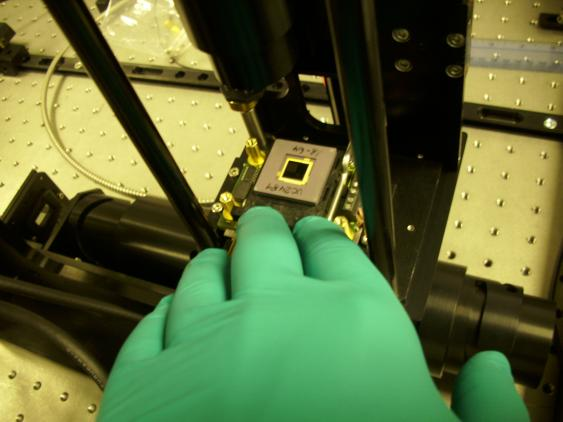
\includegraphics[width=7cm]{mma-plain}
  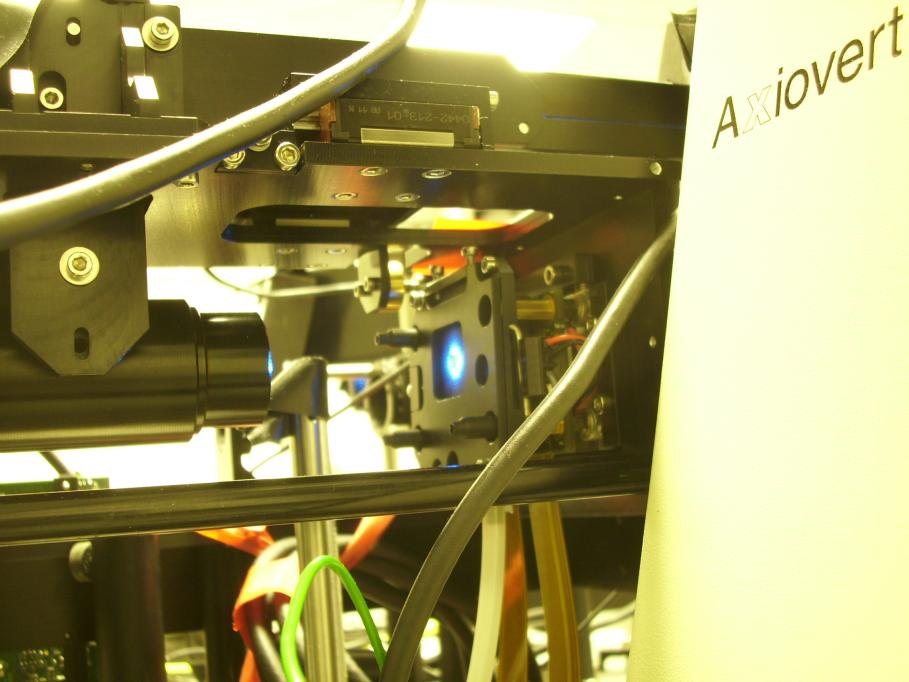
\includegraphics[width=7cm]{mma-ill}
  \caption{{\bf left:} Micro mirror array chip during installation of
    the optics. {\bf right:} Illuminated micro mirror array in the
    aligned system.}
  \label{fig:mma-closeup}
\end{figure}

\begin{figure}[!hbt]
  \centering
  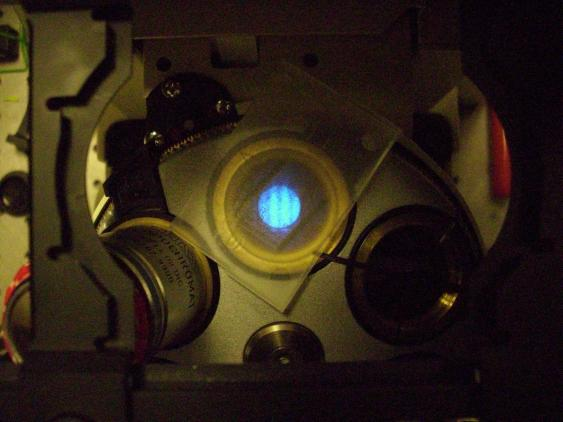
\includegraphics[width=7cm]{bfp1}
  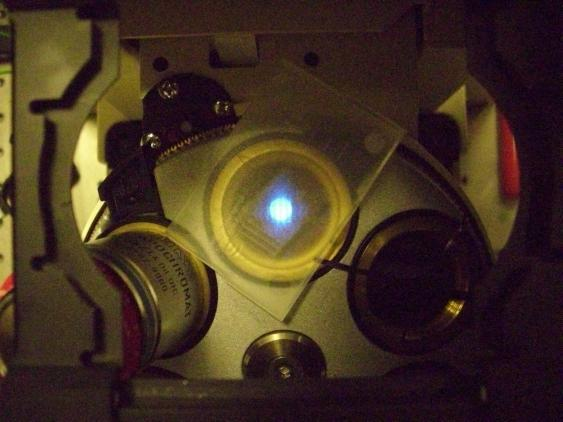
\includegraphics[width=7cm]{bfp2}
  \caption{Images of the micro mirror array in the back focal plane
    with different settings of the variable tubelens. The micro mirror
    array displays the same image (a disk) in both cases.}
  \label{fig:tubelens-bfp}
\end{figure}

\imagw{5cm}{lcos}{The black cylinder on the left is the variable tube
  lens. Behind this is the polarizing beam splitter and the
  ferroelectric liquid crystal on silicon display.}
\newpage
\section{Electronics for synchronization}
Both spatial light modulators can run at most with $50\%$ duty
cycle. Therefor it is necessary to synchronize the displays. Their
controllers allow to upload several hundred frames of image data
before an experiment and keep them in local storage. Images can then
be selected by fast function calls over USB (LCoS) or ethernet (MMA).

The camera (Andor Clara) as the slowest device is chosen as the
master. The camera provides two TTL outputs. The output ``fire'' is
high while the camera is integrating. The output ``shutter'' goes high
\unit[1]{ms} before ``fire'' and provides enough time
(\unit[$>850$]{$\mu$s}) for the MMA controller to tilt and let the
mirrors settle.

The LCoS controller can only be programmed to a limited number of
discrete image times (\unit[20]{ms}, \unit[10]{ms}, \unit[5]{ms},
\unit[200]{$\mu$s}) and it is not straight forward to change this via
USB interface. Therefor we always work with a fixed integration time
of \unit[20]{ms}. The ``fire'' output of the camera also switches the
laser on using an acousto optic modulator (AOM).

When the z-stage is used, the camera is stopped until the stage has
reached its target position.

\begin{figure}[!hbt]
  \centering
  \input{memi-electronics.eps_tex}
  \caption{The camera triggers both spatial light modulators with its
    TTL outputs. The acousto optic modulator sends light into the
    system during camera integration.}
  \label{fig:memi-electronics}
\end{figure}

\section{Alignment of the displays}

In order to be able to predict which position on the camera will be
illuminated by a particular pixel of the LCoS a calibration procedure
is run. For this a fluorescent plane is selected as a specimen. Then
single spots are scanned for a grid of $10\times10$ positions over the
LCoS. The resulting spots on the camera are located and four
parameters defining the rigid transform between camera and LCoS are
estimated (scale, rotation angle, translation in x and y, see
Appendix~\ref{sec:rigid}).

Using these parameters one can then convert between camera and LCoS
coordinates (see \figref{fig:screen_lcos-calib}). Changing the focal
length of the illumination tubelens or a change on the camera position
generally requires a new calibration.

\imagw{7cm}{screen_lcos-calib}{{\bf left:} Mask that is displayed on
  the LCoS. {\bf right:} Camera image of fluorescent plane illuminated
  by mask. The orange lines indicate the borders of the original
  pattern.}

The MMA is aligned by displaying an annular ring on the MMA and
matching it to the ring of a phase objective.


\section{Ray-based illumination optimization}
In order to make use of the spatio-angular illumination system it is
necessary to produce masks for the two spatial light modulators, that
will reduce unnecessary illumination in the sample.

\subsection{Index matched sphere model}
One useful simple model is spheres. They can model fluorescent beads
or nuclei in a \emph{C.~elegans} embryo. First we assume the beads are
embedded in index matched medium. Then rays only refract at the
gaussian sphere of the objective lens and it is insignificant how far
the target bead is from the interface between coverslip and medium
(see left drawing in \figref{fig:optimization_3}).

Suppose bead zero should be excited but the out of focus beads one to
five should not be illuminated. One could then trace the cones from
the periphery of the out of focus beads through the target points into
the back focal plane of the objective. This gives a shadow map and
when one illuminates this particular target point using this mask on
the MMA, the out of focus beads are protected.

However, the last sentence isn't true for our system. If only one
pixel of the LCoS was enabled, hardly any information of the MMA mask
would reach the back focal plane. Instead the target area should be
increased, so that the LCoS doesn't act as a pinhole.

Then several shadow maps for different target locations (e.g.\ in a
region with \unit[3]{$\mu$m} diameter) can be combined and displayed
on the MMA.  Simultaneously the LCoS should display a mask that
selects the target region. In order to suppress ringing in the focal
plane it is helpful to display a smooth image on the MMA.


\imagw{12cm}{optimization_3}{Tracing rays from the periphery of out of
  focus spheres through an in-focus target point into the back focal
  plane of the objective results in a shadow map for the MMA.}



\subsection{Index mismatch}

Biological samples are often embedded in water. For spatio-angular
illumination the additional refraction at the glass--water interface
has to be taken into account.

Analoguous to the HILO technique (see section \ref{sec:hilo}) a thin
sheet of light can be generated with an MMA mask that transmits close
to the TIRF angle. A window on the LCoS can be used to steer the beam
further. When taking into account the refractive index difference, the
depth and position of the target below the coverslip and the angle,
one can find the point on the LCoS that will giv

\begin{figure}[!hbt]
  \centering
  \def\svgscale{.3}
  \input{screen_0_lines.eps_tex} \quad \input{aberration-sketch.eps_tex}
  \caption{{\bf left:} Rays are starting from periphery of
    out-of-focus nucleus, hitting the target and refracted at the
    water--coverslip interface. {\bf right:} Due to spherical
    aberrations, rays from an on-axis point are shifted to $q(r)$ on
    the camera (where $r$ relates to the angle of the ray in the
    sample). }
\end{figure}
 
\begin{figure}[!hbt]
  \centering
  \bild{screen_microscope-aberrate}
  \caption{Raytracing through an objective followed by a tubelens. The
    focal length of the tubelens in this simulation is \unit[16]{mm}
    (as opposed to the usual \unit[160]{mm}) so that the plot fits
    into an unscaled image. The water depth is \unit[10]{$\mu$m}.}
  \label{fig:screen_microscope-aberrate-front}
\end{figure}

\chapter{Experiments}


\begin{figure}[!hbt]
  \centering
  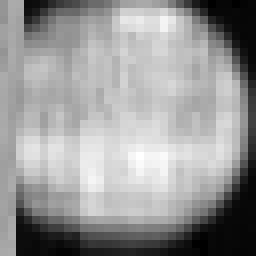
\includegraphics[width=4cm]{oil}
  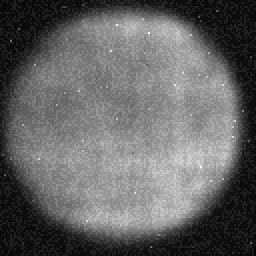
\includegraphics[width=4cm]{water}
  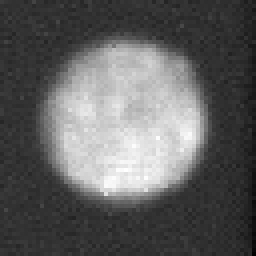
\includegraphics[width=4cm]{air}
  \caption{dfaxs}
  \label{fig:immersion-bfp-scan}
\end{figure}

\begin{figure}[!hbt]
  \centering
  \input{tirf-exp.eps_tex} 
  \caption{A fluorescent plane on a slide is embedded in oil, water or
    air. The thickness of the embedding medium is approximately
    $\unit[5]{\mu m}$. The LCoS illuminates a disk with $\unit[30]{\mu
      m}$ diameter while a $14\times 14$ window is scanned over the
    MMA.}
  \label{fig:tirf-exp}
\end{figure}


\chapter{Conclusion}
In this work we document the development of a spatio-angular
microscope. Originally we planned a fast system. That didn't work.
Because we had to run it really slow without triggers.

Now we have a system, that can potentially run fast for the image
acquisition.  But uploading images to the displays is quite slow and
limits the range of experiments that can be done. Especially its not
fun to work with and considerably hinders prototyping new illumination
schemes.

\appendix
% cascade II /mnt/backup/safe-with-time/torben/safed/y2009/0414
% andor ultra ~/1114  python code for calibration and andor basic for acquisition
\chapter{Read noise characterization in cameras}
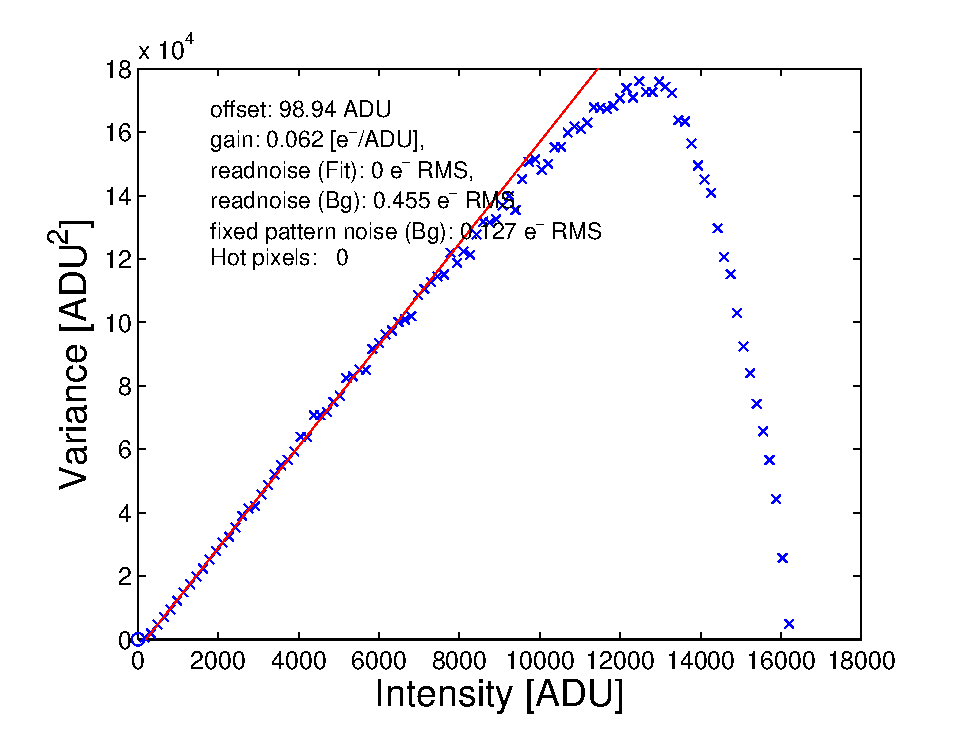
\includegraphics[width=8cm]{../app_cam/andor_emgain100_preamp5_exp30}
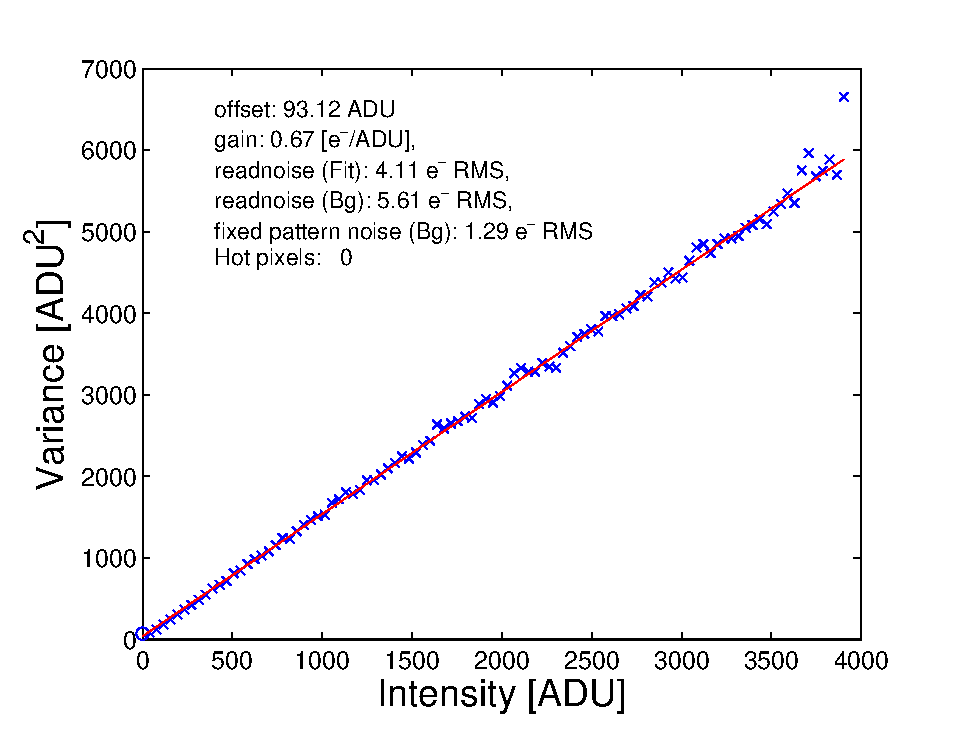
\includegraphics[width=8cm]{../app_cam/andor_normal_preamp5_exp30}
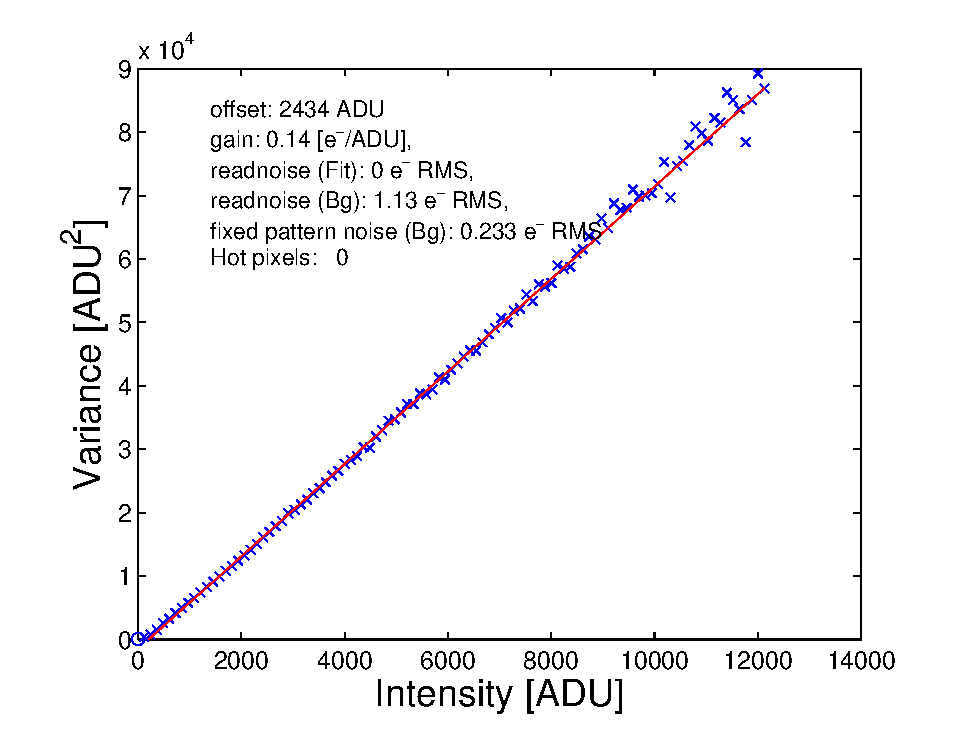
\includegraphics[width=8cm]{../app_cam/cascade_exp400ms_gain3000}
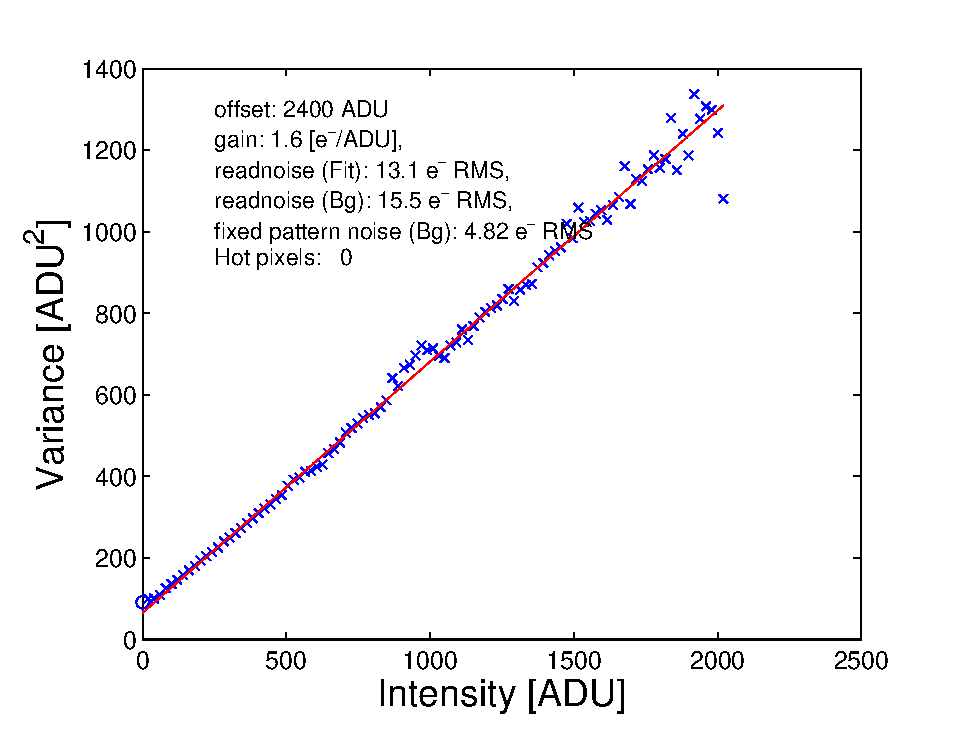
\includegraphics[width=8cm]{../app_cam/cascade_exp400ms_normal}
\includegraphics[width=8cm]{../app_cam/cascade_normal_preamp3_exp30}

% ~/from-hp2-notebook/0331/lens
% there is also code
\chapter{Raytracing for spatio-angular microscopy}
\label{sec:raytrace}
\renewcommand{\i}{\nvect i}

Here we give an overview of some useful equations for raytracing
through lens models. The design parameters of our microscope
objectives are not usually known to us. However, this is not an
unsurmountable problem as they can be represented using a simplified
model \citep{Hwang2008}. We use this to simulate the refraction at the
coverslip--medium interface for non-index matched media.

\section{Refraction at plane surface}
We begin by describing refraction at a plane surface\footnote{The
  equations are as in \citep{McClain1993}.}. The wavelength of the
light defines the length of the wave vector $\k_0$. The lengths of the
incident and transmitted wave vectors $\k_1$ and $\k_2$ are given by
the refractive index in their respective half space:
\begin{align}
  k_0&=2\pi/\lambda\\
  k_1&=n_1 k_0\\
  k_2&=n_2 k_0.
\end{align}
The normal $\n$ is directed in the opposite direction of the incident
wave vector $\k_1$. We define the transversal and normal component
vectors:
\begin{align}
  \k_{1n}&=(\k_1\n)\n\\ 
  \k_{1t}&=\k_1 - \k_{1n}.
\end{align}
Both of these components are perpendicular and during refraction the
transversal component of the wave vector is invariant:
\begin{align}
  k_2^2&=k_{2n}^2 + k_{2t}^2\\
  \k_{2t}&=\k_{1t}.
\end{align}
Using the two equations from above we can calculate the length of the
normal component of the transmitted wave vector $\k_2$:
\begin{align}
  k_2^2&=k_{2n}^2 + (\k_1 - \k_{1n})^2\\
  k_{2n}^2&=k_2^2-(\k_1-(\k_1\n)\n)^2\\
  &= k_2^2-(k_1^2-2(\k_1\n)^2+(\k_1\n)^2)\\
  &= k_2^2-k_1^2+(\k_1\n)^2.
\end{align}
Finally we can express the full transmitted wave vector $\k_2$ using
only known quantities:
\begin{align}
  \k_2&=\k_{1t}-\sqrt{k_2^2-k_1^2+(\k_1\n)^2}\n\\
  &=\k_1-(\k_1\n)\n-\sqrt{k_2^2-k_1^2+(\k_1\n)^2}\n.
\end{align}
We divide by $k_2$ with $\k_2/k_2=\t$ and $\k_1/k_2=\eta\,\i$ in order
to introduce unit direction vectors $\i$ and $\t$ for incident and
outgoing light. The relative index change across the interface is
$\eta=n_1/n_2$.
\begin{figure}
  \centering
  \input{refraction.eps_tex}
  \caption{Refraction at an interface transforms the incident wave
    vector $\k_1$ into the outgoing wave vector $\k_2$.}
\end{figure}
\begin{align}
  \t&=\eta\i-\eta(\i\n)\n-\sqrt{1-\eta^2+\eta^2(\i\n)^2}\n\\
  &=\boxed{\eta\i-\left(\eta\i\n+\sqrt{1-\eta^2(1-(\i\n)^2)}\right)\n}
\end{align}
When the radical in the square root is negative a reflection occurs
instead (TIRF). The tangential component is invariant and normal
component inverts the sign:
 \begin{align}
   \k_2&=\k_{1t}-\k_{1n}\\
   &=\k_1 - 2\k_{1n}\\
   &=\k_1-2(\k_1\n)\n\\
   \t&=\boxed{\i-2(\i\n)\n}
 \end{align}
\section{Intersection of a ray and a plane}
Let a ray start at a point $\s$ with direction $\hd$.  A plane
(defined by a point $\c$ and the normal $\n$) intersects this ray if
normal and ray direction are not perpendicular: $\n\,\hd\not=0$. The
distance between the plane and the origin is $h=\c\n$. We can define
the plane equation in Hesse normal form:
\begin{align}
  \r\n=h
\end{align}
We replace the coordinate $\r$ with the ray equation and solve for
the parameter $\tau$:
\begin{align}
  (\s+\tau\hd)\n&=h\\
  \s\n+\tau\hd\n&=h\\
  \tau&=\boxed{\frac{h-\s\n}{\hd\n}}
\end{align}
 \begin{figure}[!hbt]
   \centering
   \input{plane-intersection.eps_tex}
   \caption{Schematic for describing the plane-ray intersection.}
 \end{figure}
\section{Intersection of a ray and a sphere}
Let a ray start at a point $\s$ with direction $\hd$.  Let a sphere
sphere be centered in $\c$ with radius $R$. Their two equations
\begin{align}
  (\r-\c)^2&=R^2\\
  \r&=\s+\tau\hd
\end{align}
define the intersection points. Substitution of $\r$ results in a
quadratic equation for $\tau$:
\begin{align}
  (\s+\tau\hd-\c)^2&=R^2\\
  \l&:=\boxed{\s-\c}\\
  l^2+2\tau\l\hd+\tau^2-R^2&=0\\
  \tau^2+\underbrace{2\l\hd}_b\tau+\underbrace{l^2-R^2}_c&=0
\end{align}
\subsection{Solving the quadratic equation}
If the determinant $d$ is negative the ray misses the sphere and there
is no solution. If the determinant is zero the ray touches the
periphery and there is only one solution. A positive determinant
corresponds to two solutions. In order to prevent numerical errors the following solution should be used \citep{Press1997}: 
\begin{align}
  d&:=\boxed{b^2-4ac}\\
  q&:=\boxed{-\frac{b+\sqrt{d}\sign b}{2}}\\
  \tau&=\boxed{
  \begin{cases}
    \frac{q}{a} &\,\textrm{when}\,\abs{q}\approx 0\\ 
    \frac{c}{q} &\,\textrm{when}\,\abs{a}\approx 0\\
    (\frac{q}{a}, \frac{c}{q}) &\,\textrm{else}
  \end{cases}}
\end{align}
\section{Refraction on paraxial thin lens}
\begin{figure}[!hbt]
  \centering
  \input{lens-fwd.eps_tex}
  \caption{Construction of a ray on a thin lens. The incident beam
    with direction $\i$ hits the lens at the point $\vrho$.}
\end{figure}
The incident beam with direction $\i$ hits the lens at the point
$\vrho$. A line parallel to $\i$ through the center of the lens
defines the point on the focal plane, which will be intersected by the
transmitted ray $\r$ as well.

The triangle $ABC$ is similar to triangle $FOA$. All three angles are
identical because each of the lines are parallel:
$\overline{CB} \parallel \overline{OA} \parallel \vrho$,
$\overline{FA} \parallel \overline{CA}$ and $\overline{AB} \parallel
\overline{OF} \parallel \i$. The side $\overline{OF}$ is hypothenuse
of a right angled triangle. Its ancathete with respect to the angle
$\theta$ has length $f$. Therefor the we can deduce the length
$\abs{\overline{OF}}=f/\cos\theta$.

Between the two similar triangles, the following relation holds and
can be used to calculate the length $\abs{\overline{BC}}$:
\begin{align}
  \frac{\abs{\overline{BC}}}{\abs{\overline{BA}}}&=
  \frac{\abs{\overline{OA}}}{\abs{\overline{OF}}}\\
  \frac{\abs{\overline{CB}}}{1}&=
  \frac{\rho}{f/\cos(\theta)}.
\end{align}
Given its length, the vector $\overline{CB}$ can now calculated,
because we know its direction to be along $\vrho$. With this vector
and $\i$ we can now obtain the (arbitrarily scaled) transmitted vector
$\r'$. We could normalize it but it turns out to be useful for the
high NA immersion lens to find the vector $\r$, that ends in the focal
plane.  The procedure from above is condensed in the following
equations:
\begin{align}
  \vrho&=(x_0,y_0,0)^T=\rho (\cos\phi,\sin\phi,0)^T\\
  \phi&=\arctan(y_0/x_0)\\
  \cos\theta&=\boxed{\i\hz}\\
  \r'&=\i- \frac{\cos\theta}{f}\vrho\\
  \r&=\boxed{\frac{f}{\cos\theta} \i -\vrho}
\end{align}

\section{Refraction through oil objective (illumination)}
\begin{figure}[!hbt]
  \centering
  \input{obj-fwd.eps_tex}
  \caption{Construction of a ray on an high numerical aperture oil
    immersion objective. As opposed to a thin air lens the objective's
    focal length needs to be corrected by the focus difference vector
    $\a$ to accommodate for the immersion and we must take into
    account spherical principal surface.}
\end{figure}
It is possible to augment the results of the calculation from the
previous chapter to treat an aplanatic immersion objective
\citep{Hwang2008}.

We account for the immersion medium by shifting the focal plane in
sample space to $nf$ using the focus difference vector $\a$.
\begin{align}
  \a &= \boxed{f (n-1) \hz} \\
  R &= \boxed{nf}
\end{align}
The principal surface\footnote{An image forming system focusses
  parallel light into a point. Its prinicipal surface is the surface
  where an incident parallel ray intersects with a line along the
  transmitted image forming ray.} is a sphere of radius $R=nf$ around
the image point (\cite{Smith2000} p.~22). In the paper
\citep{Hwang2008} they express the deviation between the real
principal surface and the principal plane with an approximation for
small angles $\theta$ and $\phi$:
\begin{align}
  \s &= \boxed{(R - \sqrt{R^2-\rho^2})\i}
\end{align}
This is an approximation because it only takes into account the
perpendicular (along $\z$) distance between plane and sphere. They
demonstrate the viability of this approximation by comparing its
results with a full raytrace through a $100\times\,1.41$
objective. Focus displacement errors are less than \unit[130]{nm} for
a field of $\unit[86.4]{\mu m}$ radius. This is sufficient for our
problem. As we anyway have the code for a ray--sphere intersection, we
can use it here as well and calculate an exact vector $\s$.

The final ray exiting the objective has the direction $\r_0$:
\begin{align}
  \r_0 &= \boxed{\r + \a - \s}.
\end{align}
\section{Reverse path through oil objective (detection)}
Now we consider the oil objective in the reverse direction (see
\figref{fig:obj-ref-full}). We have a ray starting within the sample
and want to know the transmitted ray in the pupil.

\subsection{Easy case: back focal plane positions only}
If we are only interested in positions of rays in the back focal
plane, we don't have to do full raytracing. If we are imaging beads in
index matched embedding medium and we want to calculate shadow maps
for the MMA (see section \ref{sec:shadow-map}), we don't need a full
raytrace. Instead it is sufficient to ignore ray origins and just
consider their directions.

A unit ray direction $\i=(x,y,z)^T$ in sample space is transformed
into a position $\r_b=(x',y')^T$ in the back focal plane of the
objective. The azimuthal angle $\phi$ isn't changed when going through
the objective. The polar angle $\theta$ defines how far off axis the
back focal plane is hit.
\begin{align}
  \phi'&=\phi=\arctan(y/x)\\
  \theta&=\arcsin(\sqrt{x'^2+y'^2})\\
  r_b&=nf\sin\theta\\
  \r_b&=r_b(\cos\phi',\sin\phi')^T
\end{align}
 \begin{figure}[!hbt]
   \centering
   \input{obj-rev.eps_tex}
   \caption{Schematic for tracing a ray direction $\i$ from sample
     space into the back focal plane. The bigger the angle between
     $\i$ and the optical axis, the further outside the ray will pass
     through the back focal plane.}
 \end{figure}
\subsection{Full raytrace}
If we are also interested in the angles of the transmitted rays in the
back focal plane, when we want to trace the rays further into the
camera or if we want to consider aberrations due to an index mismatch
of the embedding medium, we will have to calculate a full raytrace, as
describted below.

The position of the objective is defined by its principal point $\c$
and the normal $\n$ (directed along optical axis towards sample
space). The incident ray is defined by its starting point $\p$ and the
direction $\i$. First we calculate the center of the gaussian sphere
$\vect g$:
\begin{align}
  \vect g &= \c + nf \n.
\end{align}
Then we obtain the position $\p'$ by intersecting the incident ray and
the plane perpendicular to the optical axis through $\vect{g}$.  The focus
difference vector is defined by its length and the optical axis. It
can be used to calculate an intermediate point $\p''$.
\begin{align}
  \a &= -f(n-1)\n \\
  \p'' &= \p' + a.
\end{align}
The point $\p''$ has now been shifted, so that a thin air lens would
image it exactly as the oil objective would image $\p'$. We can use
$\p''$ to find the direction $\t$ of the transmitted ray. It is just
the normalized difference vector $\vect m$ to the principal point.
\begin{align}
  \vect m &= \c - \p'' \\
  \t &= \vect m / \abs{\vect m}.
\end{align}
As a last step we calculate the starting point $\e$ of the transmitted
ray by intersecting the incident ray with the gaussian sphere.
\begin{figure}[!hbt]
  \centering
  \input{obj-rev-full.eps_tex}
  \caption{Construction to find the transmitted ray through an oil
    immersion objective from a point within the sample.}
  \label{fig:obj-ref-full}
\end{figure}
\subsection{Treatment of aberration (detection)}
Now we consider a ray originating in point $\p$ with direction $\i$
within an immersion of index $n_e$. We want to treat the problem of a
non-matched embedding medium $n_e\not=n$. We find the intersection
$\f$ of the ray with the coverslip--embedding interface and refract to
obtain $\i'$. We calculate the time $t$ a photon takes, to travel from
$\p$ to the interface $\p$:
\begin{align}
  t = \abs{\f - \p} n_e c
\end{align}
and extend the path of the photon backward along $\i'$ by
$t/(cn)$. This results in the corrected position $\p'$ that indicates
where the photon would have originated if the embedding would have
been index matched.  Now we can apply the equations from the previous
sections on the ray defined by $\p'$ and $\i'$ to obtain the
transmitted ray in the pupil.

 \begin{figure}[!hbt]
   \centering
   \input{obj-rev-full-emb.eps_tex}
   \caption{Construction that treats the interface between embedding
     and immersion medium}
 \end{figure}
\section{Sphere projection}
When we model our sample as a collection of spheres, it is useful to
trace rays from the periphery of these spheres through an in focus
target $\c$ into the back focal plane. Here we construct the rays.

The tangents of an out of focus sphere $S^\s_r$ centered at $\s$ with
radius $r$ that pass through the target $\c$ form a double cone
(assuming $\c$ is outside of $S^\s_r$. The tangents touch the surface
of the sphere $S^\s_r$ at the circular intersection $C$ with the sphere
$S^\c_R$ centered at $\c$ with radius $R=\abs{\c-\s}$. Radius $R$ is
the distance from the target to the center of the out of focus sphere.
\begin{figure}[!hbt]
  \centering
  \input{touch-cone.eps_tex}
  \caption{Schematic of how an out of focus nucleus defines a cone of
    tangential rays.}
\end{figure}
In order to find a point $\e$ where a tangent touches the out of focus
sphere, it is sufficient to solve the following equation in a 2D
coordinate system with the origin in the center $\s$ of the out of
focus sphere:
\begin{align}
  (x-R)^2+y^2&=R^2\\
  x^2+y^2=r^2
\end{align}
There are two solutions:
\begin{align}
  x_1&=\frac{r^2}{2R}\label{eqn:x1}\\ 
  y_{1/2}&=\pm\frac{r}{2R}\sqrt{4R^2-r^2} \label{eqn:y1}
\end{align}
In the case $R<r$ the out of focus nucleus is intersecting the target,
obliviating the reason to do the projection in the first place.

We construct two vectors $\hx$ and $\hy$ in order to transform the
solution from 2D into 3D. The (unnormalized) direction $\x$ of the
x-axis of this coordinate system is given by the difference vector of
the target $\c$ and the nucleus center $\s$. The direction $\y$ must
be perpendicular to $\x$ and is obtained by calculating the cross
product with another vector $\q$.  We ensure that $\q$ and $\x$ are
not colinear. The vectors $\q$ and $\x$ are colinear, when the
absolute value of their scalar product equals the square of the length
$\abs{\q\x}=\x^2$.
\begin{align}
  \x&=\c-\s\\
  \q&=\begin{cases}
    (0,0,1)^T & \textrm{when}\ \abs{x_z}<\frac{2}{3}\abs{\x}\\
    (0,1,0)^T & \textrm{else}
  \end{cases}\\
  \y&=\x\times\q \\
  \hx&=\x/\abs{\x}\\
  \hy&=\y/\abs{\y}
\end{align}


Now we can sample the intersection circle $C$ in order to create
viable starting points $\e$ for tangential rays.  Let $R_\phi^\hc$ be
a rotation matrix that rotates a vector by angle $\phi$ around an axis
$\hc$. A point $\e$ on the circle is then defined using one solution
from equations \ref{eqn:x1} and \ref{eqn:y1}. The ray direction $\f$
is then easily obtained:
\begin{align}
  \e&=\s+x_1\hx+y_1R_\phi^\hx\hy\\
  \f&=\c-\e.
\end{align}
Tracing a sufficient number of rays (e.g.\ 16) with direction $\f$ for
different angles $\phi$ to the back focal plane gives the projection
of the intersection circle $C$. Note that this projection in general
is not a circle anymore.

For practical reasons its useful to project vector $\x$ as well. It
can be used as the center of the (distorted) shape on the back focal
plane to rasterize it as a fan of triangles.

\section{Defocus due to aberrations}
\begin{itemize}
\item think of a photon traveling along the optical axis from
  objective towards sample (see \figref{fig:aberration-sketch})
\item in the unaberrated case the focal plane would be at the center
  of the gaussian sphere at $nf$ optical length from intersection of sphere
  with optical axis
\item in the aberrated case the optical length inside glass/oil is $n(f-h)$,
  where $h$ is the water depth; the optical length in water is $n_eh$
\item we are interested in how the displacement $q$ varies with the
  intersection $r$ of the ray in the back focal plane (for a defined
  water depth $h$) (see \figref{fig:focus-displacement} for results of
  a simulation)
\item here we only show the result an on-axis point in the sample,
  shifting the sample doesn't seem to influence the shape of $q(r)$
\item the maximum value for $r$ is $R_\textrm{BFP}=f\textrm{NA}$
\item notice that $q(r)$ isn't bijective, rays that leave the sample
  in a very high angle are bent more than rays of moderate angle (see
  also \figref{fig:screen_microscope-aberrate})
\item {\color{red}for our application this means that if the MMA is
    adjusted to bright at the border of the back focal plane a bright
    spot on the LCoS will lead to two discrete illumination angles.}
  this could potentially be a problem
\item the simulation can be quite wrong for high angles as the
  coverslip will probably not be perfectly plane
\item the zoomed plot in \figref{fig:screen_microscope-aberrate} shows
  the focus displacement for moderate angles that exit the sample
\item the aberrations are stronger when the sample is embedded deeper
  in water
\item for a water depth of \unit[100]{$\mu$m} a ray that intersects
  the back focal plane at \unit[2]{mm} distance off-axis is shifted by
  \unit[0.5]{mm} in the image (\unit[8.2]{$\mu$m} in the sample)
\item rays further off-axis are aberrated even more
\end{itemize}
\begin{figure}
   \centering
   \input{aberration-sketch.eps_tex}
   \caption{Schematic depicting the variables involved in focus
     displacement due to aberrations at a water-coverslip
     interface. The variable $h$ is the depth of the water, $q$ is the
     focus displacement in the image.}
   \label{fig:aberration-sketch}
 \end{figure}
 
\begin{figure}[!hbt]
  \centering
  \bild{screen_microscope-aberrate}
  \caption{Raytracing through an objective followed by a tubelens. The
    focal length of the tubelens in this simulation is \unit[16]{mm}
    (as opposed to the usual \unit[160]{mm}) so that the plot fits
    into an unscaled image. The water depth is \unit[10]{$\mu$m}.}
  \label{fig:screen_microscope-aberrate}
\end{figure}

\begin{figure}[!hbt]
  \centering
  \bild{../raytrace/focus-displacement}
  \bild{../raytrace/focus-displacement-zoomed}
  \caption{Plot of the focus displacement of a point on the optical
    axis for rays that intersect the back focal plane in different
    positions. The tubelength for this simulation was
    \unit[160]{mm}. Note that rays the intersect the back focal plane
    at \unit[50]{mm} distance to the optical axis don't enter the
    tubelens. Parameters: the objective focal length is
    \unit[2.61]{mm}, the tubelength is \unit[160]{mm}, the immersion
    index is $n=1.52$ and the embedding index is $n_e=1.33$ }
  \label{fig:focus-displacement}
\end{figure}
\def\NA{\textrm{NA}}

\newpage
\section{Test}
Set the target point $\c=(0,0,0)^T$ and the nucleus center to
$\s=\unit[(-6,0,-7)^T]{n_e \mu m}$ with a nucleus radius
$r=\unit[1.2]{n_e \mu m}$. Note that dimensions are \emph{optical}
path lengths and must be multiplied with the refractive index
$n_e=1.33$. 

\begin{figure}[!hbt]
  \centering
  \input{projection-schematic.eps_tex}
  \caption{Schematic that indicates placement of different optical
    entities for the projection simulation.}
  \label{fig:projection-schematic}
\end{figure}


The focal length of the tubelens is $f_\textrm{TL}=\unit[164.5]{mm}$
and the objective's is $f=f_\textrm{TL}/63=\unit[2.61]{mm}$. The
numerical aperture of the objective is $\textrm{NA}=1.38$. The radius
of the back focal plane is $R=f \NA=\unit[3.6]{mm}$.

We set the waterdepth to $h=\unit[10]{\mu m}$. The immersion index is
$n=1.52$. The focal plane is therefore at the following distance $d$
left of the objective center:
\begin{align*}
  d&=n_eh+n(f-h)\\
  %&=\unit[(1.33*.01+1.52*(164.5/63-.01))]{mm}\\
  &=\unit[3.9669]{mm}
\end{align*}
as opposed to $nf=\unit[3.9688]{mm}$ for an unabberated objective. The
water layer shifts the focus axially by \unit[1.9]{$\mu$m} in the
simulation coordinate system.


\begin{figure}[!hbt]
  \centering
  \bild{screen_1}
  \caption{Rays from the out-of-focus nucleus are projected into the
    back focal plane. The area they circumscribe shouldn't be
    illuminated in order to protect the out-of-focus nucleus from
    exposure. The red area of the gaussian sphere corresponds to
    angles that are collected by the objective.}
  \label{fig:rays-from-out-of-focus}

%FIXME maybe compare to ./cyberpower-store/0314/zeiss-patents/20080106795-correction-ring.pdf 
%or US7268953-63x.pdf

\end{figure}


% 0609/scan
\chapter{Transforming camera coordinates into LCoS coordinates}
\label{sec:rigid}
\begin{summary}
  In our microscope the plane of the camera is conjugate to the plane
  of the LCoS display. It is useful and for most illumination
  strategies crucial to be able to relate a camera position back to
  the LCoS. Then the information from one exposure can be used to
  control the illumination in the next.

  Whenever the camera is moved or the variable tubelens is changed, we
  have to recalibrate the system with a fluorescent plane sample on
  which we project single spots with known positions on the LCoS. Here
  we describe a robust approach to find a rigid transform between LCoS
  and camera coordinates.
\end{summary}
\section{Description of the rigid transform}
In order to relate coordinates on the LCoS display with pixel
positions on the camera, we found it suffices to use a rigid
transform. The rigid transform between display and camera is defined
as:
\begin{align}
  \r^d&=s \textrm{R}_\phi \r^c + \vect t\\
  \textrm{R}_\theta&=\begin{pmatrix}
  \cos\phi & q\sin\phi \\
  -\sin\phi & q\cos\phi \\ 
  \end{pmatrix}
\end{align}
where $\r^d$ is a point on the display, $\r^c$ is a point on the
camera and $q$ can be either $+1$ or $-1$. The value of $q$ is $-1$,
if there is a reflection. It is $+1$ if there is no reflection.

\begin{figure}[!hbt]
  \centering
  \input{calib-align.eps_tex}
  \caption{Given $n\ge 4$ camera images of a display showing one
    point.  It is possible to calculate the parameters of the rigid
    transform parameters scaling $s$, rotation angle $\phi$,
    translation vector $\vect t$.}
  \label{fig:calib-align}
\end{figure}



One can find the transform parameters scaling $s$, rotation angle
$\phi$, translation vector $\vect t$ by minimizing
\begin{align}
  \sum_i^n \abs{s \textrm{R}_\phi \r^c_i+\vect t -\r^d_i}^2 \label{eq:rigid-sum}
\end{align}
for all $n$ points on the display $\r^d_i$ and there corresponding
camera positions $\r^c_i$.  Each term of the sum can be expressed as
two scalar terms:
\begin{align*}
  \sum_i^n&
  \abs{s(\cos\phi r^c_{ix}+q\sin\phi r^c_{iy})+t_x-r^d_{ix}}^2
  +
  \abs{s(-\sin\phi r^c_{ix}+q\cos\phi r^c_{iy})+t_y-r^d_{iy}}^2
\end{align*}

The following Maxima code will find the solution to the least squares
problem:
\begin{verbatim}
load(minpack)$
q:-1;
g(s,p,tx,ty):=[s*( cos(p)*<cx>+q*sin(p)*<cy>)+tx-<dx>,
               s*(-sin(p)*<cx>+q*cos(p)*<cy>)+ty-<dy>, ... ]$
minpack_lsquares(g(s,p,tx,ty), [s,p,tx,ty], [0.88,-3.1,1200,-20]);
\end{verbatim}
We define the function \verb!g! to contain all the terms of the sum.
This can easily written by a program that constructs the lines
according to the given pattern, replacing \verb!<cx>!, \verb!<cy>!
with camera coordinates and \verb!<dx>!, \verb!<dy>! with display
coordinates.

The function \verb!minpack_lsquares! calls the subroutine \verb!lmder!
which was originally developed for the Fortran\footnote{Rather than
  calling a Fortran library Maxima calls a version of this function
  that was automatically translated into Common Lisp via {\sf f2cl}.}
package \verb!minpack!.

{\small
\begin{verbatim}
c     subroutine lmder (http://www.netlib.org/minpack/lmder.f)
c     the purpose of lmder is to minimize the sum of the squares of
c     m nonlinear functions in n variables by a modification of
c     the levenberg-marquardt algorithm. the user must provide a
c     subroutine which calculates the functions and the jacobian.
c     the subroutine statement is
c       subroutine lmder(fcn,m,n,x,fvec,fjac,ldfjac,ftol,xtol,gtol,
c                        maxfev,diag,mode,factor,nprint,info,nfev,
c                        njev,ipvt,qtf,wa1,wa2,wa3,wa4)
\end{verbatim}
}

\noindent The reason for using Maxima is, that it calculates the symbolic
Jacobian for the problem. This makes it straight forward to change the
simple rigid transform to a model with more parameters.

The following Common Lisp code shows how the result of the
optimization can be used to initialize the OpenGL modelview matrix to
transform objects in its buffer, so that they will appear at the given
positions on the camera.

{\small
\begin{verbatim}
(defun load-cam-to-lcos-matrix (&optional (x 0s0) (y 0s0))
  (let* ((s 0.828333873909549) (sx  s)        (sy  (- s))
         (phi -3.102)          (sp (sin phi)) (cp (cos phi))
         (tx 608.433)          (ty 168.918)
         (a (make-array (list 4 4) :element-type 'single-float
             :initial-contents
             (list (list (* sx cp)    (* sy sp)  .0   (+ x tx))
                   (list (* -1 sx sp) (* sy cp)  .0   (+ y ty))
                   (list .0           .0        1.0   .0)
                   (list .0           .0         .0  1.0)))))
    (gl:load-transpose-matrix (sb-ext:array-storage-vector a))))    
\end{verbatim}
}
  

\noindent
Alternatively, here is the equivalent code in C:

{\small
\begin{verbatim}
float m[4*4]; // OpenGL Modelview Matrix
float s=-.8749328910202312,
      sx=s,sy=-s,phi=-.8052030670943575,
      cp=cos(phi),sp=sin(phi),
      tx=1456.71806436377,
      ty=910.4787738693659;
  m[0]=   sx*cp;   m[4]=sy*sp;   m[8] =0;    m[12]=tx; 
  m[1]=-1*sx*sp;   m[5]=sy*cp;   m[9] =0;    m[13]=ty; 
  m[2]=0;          m[6]=0.;      m[10]=1;    m[14]=0;  
  m[3]=0;          m[7]=0.;      m[11]=0;    m[15]=1;  
glMatrixMode(GL_MODELVIEW);
glLoadMatrixf(m);
\end{verbatim}
}
\section{Experimental example and image processing}

For the calibration a fluorescent plane (see
\figref{fig:rigid-pics}~left for a uniform wide field image) is imaged
with the LCoS display showing spots in the illuminated area.  Ideally
for this measurement all mirrors on the MMA are undeflected and the
apertures $B_0$ and $B_1$ completely open (see
\figref{fig:memi-real}). Then the square exit of the integrating
tunnel illuminates the biggest possible area on the LCoS.

\begin{figure}[!hbt]
  \centering
  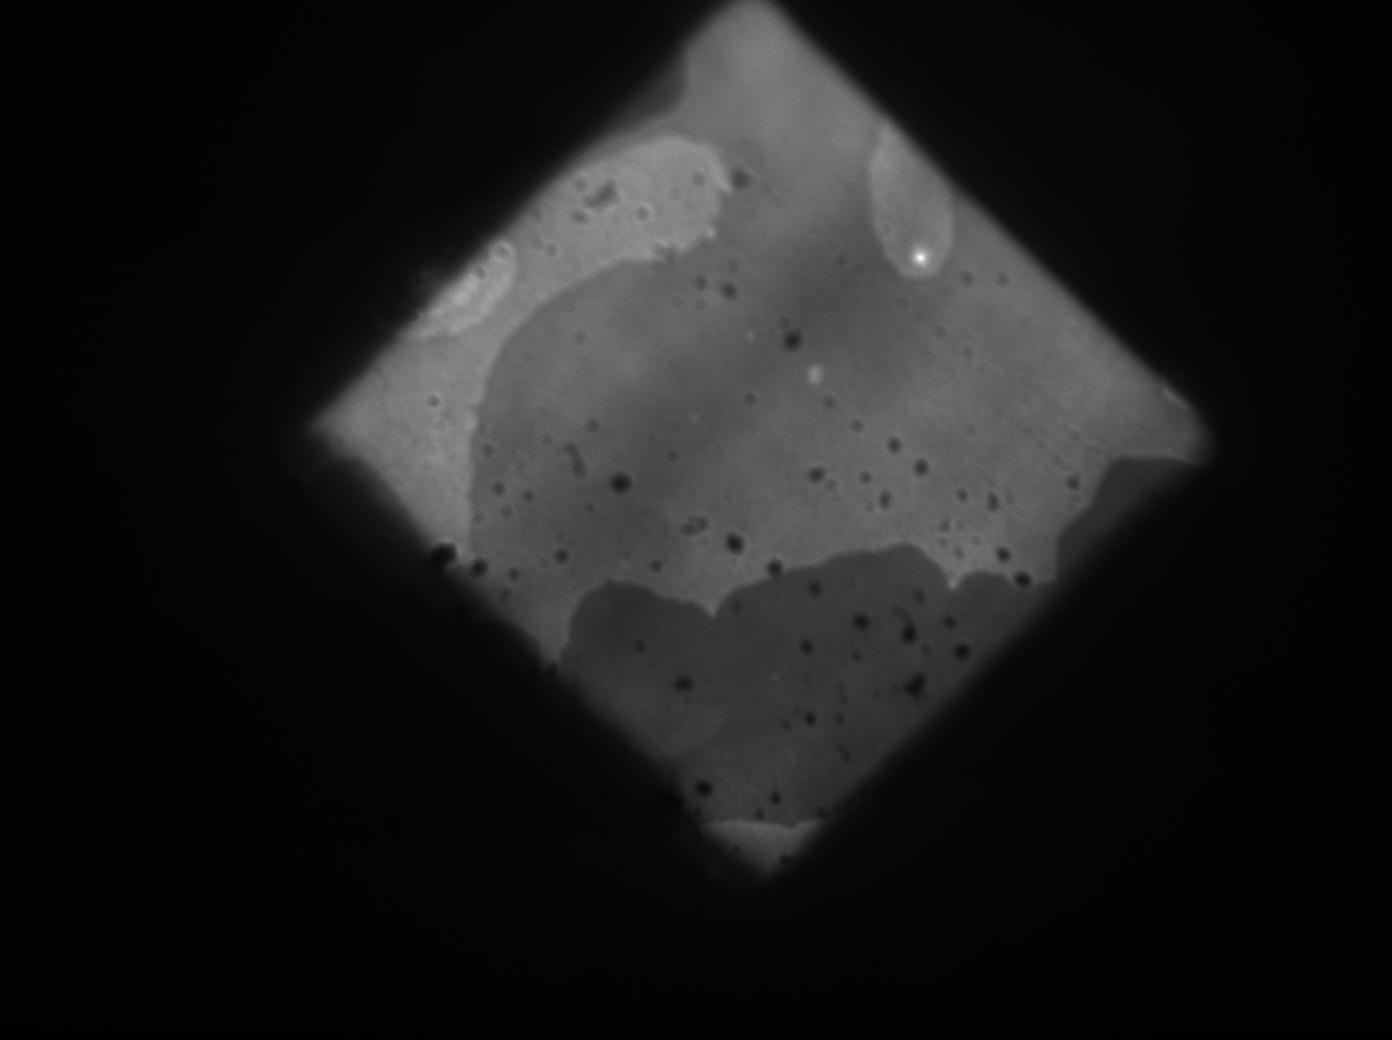
\includegraphics[width=7cm]{o102}
  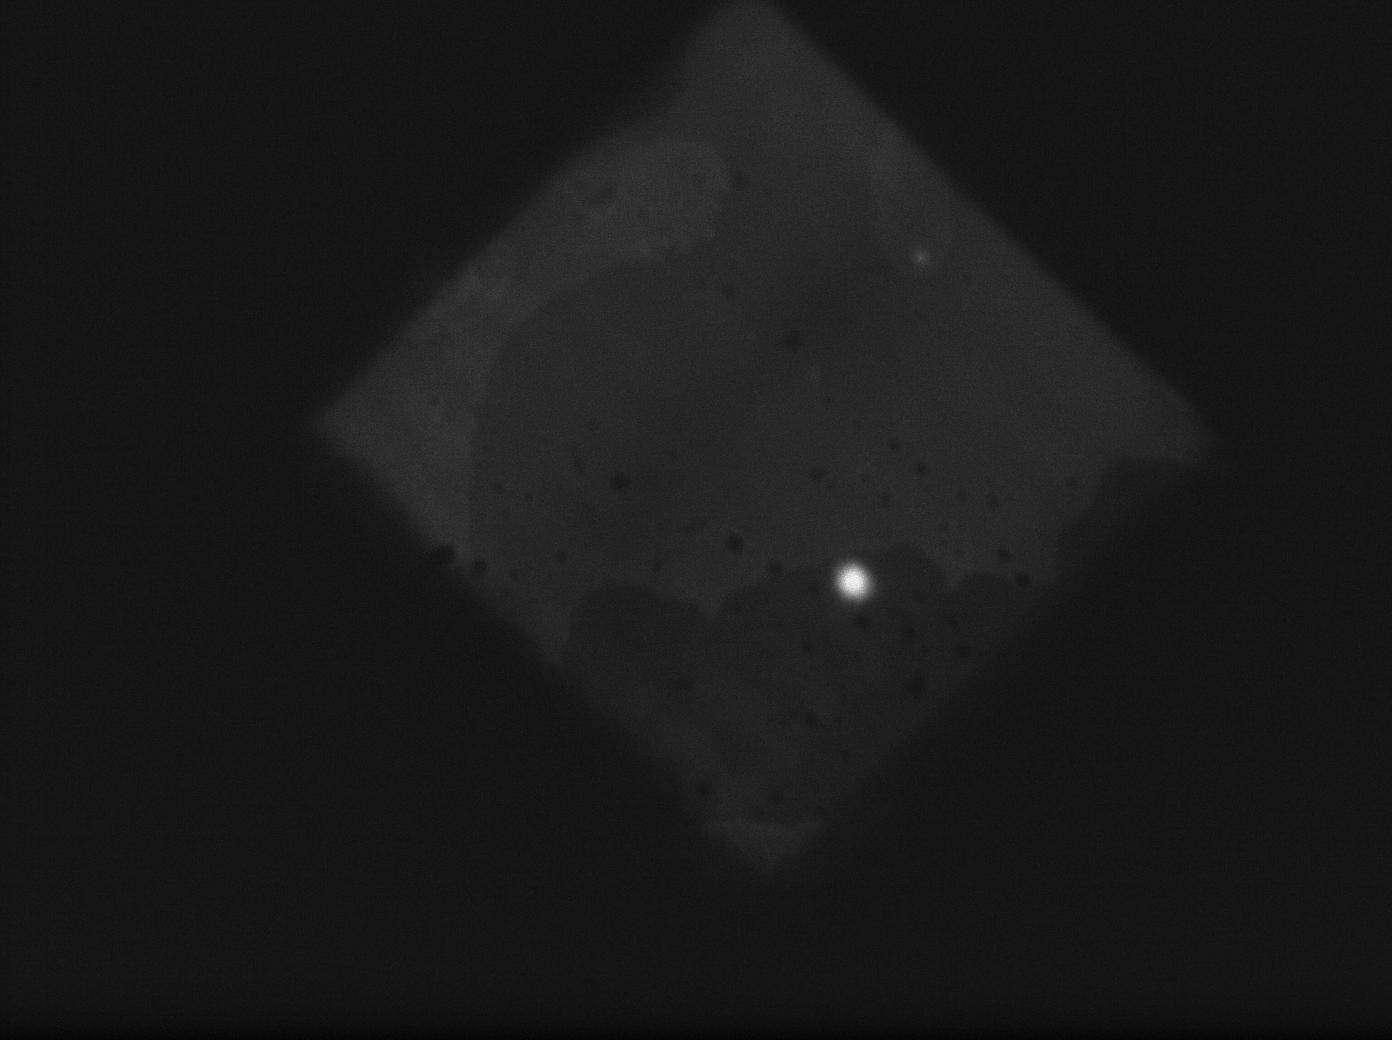
\includegraphics[width=7cm]{o035}
  \caption{{\bf left:} Uniformly illuminated fluorescent plane (mono
    and double layer of yellow beads with \unit[110]{nm} diameter,
    excited with \unit[473]{nm} laser in a 63x/1.47 objective). {\bf
      right:} Image with the the LCoS displaying a disk with 24 pixels
    diameter (corresponding to $\unit[2.4]{\mu m}$ in the sample)
    centred at LCoS position $(550,750)$.}
  \label{fig:rigid-pics}
\end{figure}

% i believe the TL_ill is set to r_MMA=3.84mm in BFP 
% f_TLill = 352 mm
% mag_real = mag / f_zeiss * f_TLill 
% pixel-pitch-lcos / mag_real
% one pixel is: 13.62 / 63 * 164.5 / 352 = 101nm

\begin{figure}[!hbt]
  \centering
  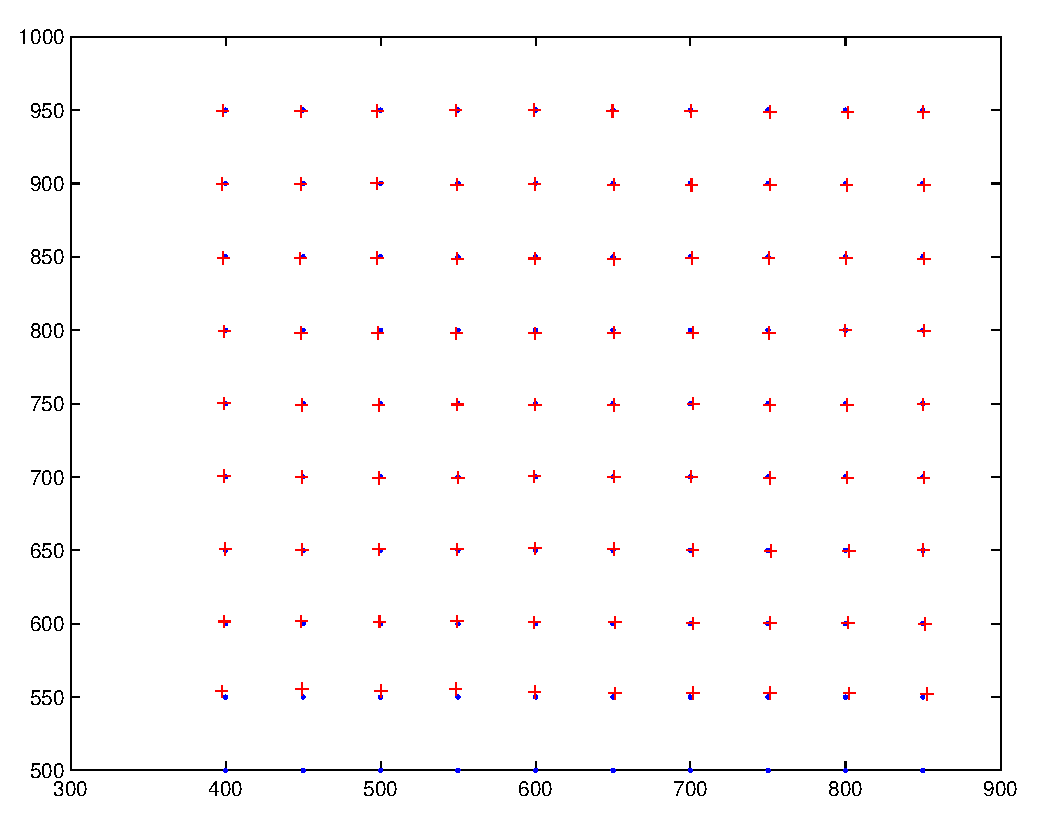
\includegraphics[width=12cm]{../rigid/rigid-compare}
  \caption{Red ``$+$'' signs indicate where the spots that were
    localized in the camera images end up after a rigid
    transform. There is sufficient agreement with the original
    display positions.}
  \label{fig:rigid-compare}
\end{figure}

For the calibration $10\times10$ images (100 images, each containing
one bright spot at a different position) were captured with a disk of
24 pixels diameter at the positions $(400+50i,500+50j)\ \forall i,j\in
[0,99]$. Furthermore, one uniformly illuminated image is used to
correct for intensity fluctuations in the fluorescent plane.  The
following Matlab/DIPimage code is used to normalize the images and
localize the spots. The coordinates are then assembled into the Maxima
command that finds the parameters of the rigid transform. Finally the
transformed spot positions from the camera images are compared with
the original LCoS pixel positions.

The following Matlab listing shows how to open the image files:
% cd /mnt/scan 
{\small
\begin{verbatim}
%% load the files
% 0 .. 99 spot images
% only 10..99 usable because the first are on border and not illuminated
a = newim(1392,1040,103);
for i=0:102
    % Andor's FITS format isn't read correctly
    % correct this by adding 2^15
    a(:,:,i) = 2^15 + readim(sprintf('o%03d.fits',i));
end
\end{verbatim}}

  Of the 103 images, that are loaded into \verb!a!, the first 100
  contain spots and the image at the zero-based index 102 is the
  uniformly illuminated image shown in \figref{fig:rigid-pics} left.
  The other two images at indices 100 and 101 are two centered disks
  with different diameters and are not used here.

{\small
\begin{verbatim}
bright = squeeze(a(:,:,102));  % histogram of uniformly illuminated
                               % image has minimum at 800 ADU
mask = gaussf(bright,8) > 800; % create mask with illuminated area
bg = 510;                      % the background is be 510 ADU

posmax = newim(100,2);
for i = 10:99
    % correct for sample non-uniformity 
    corr = (squeeze(a(:,:,i)) - bg) / bright * mask;
    % find coordinates of maximum
    [coords,vals]=findmaxima(gaussf(corr,32));
    [valss,valsind] = sort(vals);   % sort coordinates by intensity
    tmp = coords(valsind,:);        % collect the maximum with highest
    posmax(i,:) = tmp(end,:);       % intensity into result
end
\end{verbatim}}
  
  The DIPimage toolbox provides the function \verb!findmaxima!, that
  locates all local maxima in an image with subpixel accurac y. We
  sort the result by gray value and only use the biggest.  The
  measured 100 camera coordinate pairs in \verb!posmax! correspond to
  $\r^c_i$ in equation \ref{eq:rigid-sum}.
 
  From Matlab we create the file \verb!fit.max! with batch commands
  for Maxima. Then we run Maxima. When it is finished after a few
  seconds, the file \verb!max.out! will contain the four fitted
  parameters.
 
{\small
\begin{verbatim}
c = double(posmax)';
cmd = '';                       % collect equations in maxima format
for i=10:99
    dx = num2str(400+50*mod(i,10));
    dy = num2str(500+50*floor(i./10));
    cx = num2str(c(i+1,1)); 
    cy = num2str(c(i+1,2));
    cmd=[cmd ' s*( cos(p)*' cx '+q*sin(p)*' cy ')+tx-' dx ', ...
         s*(-sin(p)*'cx '+q*cos(p)*' cy ')+ty-' dy ','];
end
cmd(:,end) = []; % delete last comma

% load the fitting package and start defining the merit function g
pre = 'load(minpack)$ q:-1; g(s,p,tx,ty):=[';
% now put cmd between
% call the fitting function and store the parameters into max.out
cod = [']$ fit:minpack_lsquares(g(s,p,x,y),[s,p,x,y],[.88,-1.3,1200,-20]);' ...
 'write_data(fit[1],"max.out");']

fid = fopen('fit.max','w'); % write maxima commands into file 
fwrite(fid,[pre cmd cod]);
fclose(fid);
[max_status,max_result]=system('maxima -b fit.max');  % execute maxima
\end{verbatim}}

  We load the transformation parameters back into Matlab and create
  the diagram \figref{fig:rigid-compare} to visualize, how well the
  transform matches camera and display coordinates.

{\small
\begin{verbatim}
% load rigid transformation parameters from the file into matlab
params = load('max.out')'; 
scale = params(1); phi = params(2);
tx = params(3);    ty = params(4);

mirr = -1;
R = [cos(phi),mirr*sin(phi);
     -sin(phi),mirr*cos(phi)];
T = [tx ty]';

%% plot the two grids on top of each other
mapped = zeros(100,2);
for i=11:100 % camera coordinates into display coordinates
    mapped(i,:) = (scale*R*q(i,:)'+T)';
end

dpos = zeros(100,2);
for i=0:99 % calculate display points
    dpos(i+1,1) = 400+50*mod(i,10);
    dpos(i+1,2) = 500+50*floor(i./10);
end

hold off;  plot(dpos(:,1),dpos(:,2),'.');
hold on;   plot(mapped(11:end,1),mapped(11:end,2),'r+');
\end{verbatim}}
% print -depsc2 /home/martin/thesis/kielhorn/rigid/rigid-compare

\section{Conclusion}
The rigid transform and our method to estimate its parameters is a
sufficient and robust method, to map the coordinates of our camera
into those of the spatial display.

The rigid transform can be done directly in OpenGL. Hence, it is
trivial to render a properly transformed texture of the camera
image which is then shown on the display.

An advantage over other methods, e.g. finding a homology matrix via
RANSAC, is that the result is not a transformation matrix but
separated parameters for scaling, rotation and translation. 


\definecolor{listinggray}{gray}{0.9}
\definecolor{lbcolor}{rgb}{0.9,0.9,0.9}
\lstset{
	backgroundcolor=\color{lbcolor},
	tabsize=4,
	rulecolor=,
	language=matlab,
        basicstyle=\sffamily\footnotesize, %\scriptsize,
        upquote=true,
        aboveskip={1.5\baselineskip},
        columns=fixed,
        showstringspaces=false,
        extendedchars=true,
        breaklines=true,
        prebreak = \raisebox{0ex}[0ex][0ex]{
          \ensuremath{\hookleftarrow}},
        frame=single,
        showtabs=false,
        showspaces=false,
        showstringspaces=false,
        identifierstyle=\sffamily,
        keywordstyle=\color[rgb]{0,0,1},
        commentstyle=\color[rgb]{0.133,0.545,0.133},
        stringstyle=\color[rgb]{0.627,0.126,0.1},
}
\newcommand{\avg}[1]{\langle #1 \rangle}

\chapter{Implementation of a robust structured illumination
  reconstruction technique}
\label{sec:app_hilo}
\begin{summary}
  We implement a robust technique to computationally recover optically
  sectioned images from only two structured illumination images.
\end{summary}
\section{Wave optical model of microscope}
The resolution of an objective is related to the angles of light, that
are collected by the lens. For a good introduction see
\citet{Gustafsson1995}.

A Fourier transform separates the electric field amplitude $E(\r)$ of
light into plane wave components. If the light is monochromatic, then
all the plane waves have the same wavelength but different directions.

The wave vectors of the electric field amplitude $\tilde E(\k)$ lie on
a spherical shell in the three-dimensional k-space. The radius of the
sphere is $k=2\pi/\lambda$. A lens only selects a limited part of the
wave vectors and thereby looses information about the sample.

The same is true for illumination. When a plane monochromatic wave
enters the objective from the back focal plane, the lens ``bends''
rays towards the focus. The Fourier components travelling towards the
focus are again limited by the numerical aperture of the lens and
$\tilde E(\k)$ is defined only on part of the spherical shell or a
bowl-shape in $\k-$space.

The excitation of fluorophores is proportional to the intensity.  The
intensity is the absolute square $\abs{E(\r)}^2$ of the field. This
can also be expressed as the product of the field and its complex
conjugate $E(\r)E^*(\r)$. In Fourier space this product turns into the
convolution $\tilde E(\k)\otimes\tilde E(-\k)$, i.e.\ a bowl is drawn
with an upside-down bowl. This explains the simple graphical
construction in \figref{fig:missing-cone} for the support of the OTF.

\section{Simulated image acquisition}
As a test object we create a thick sphere shell, a line and a
rectangle. The sphere shell will provide out-of-focus light, which we
then try to remove. We simulate the illumination through an objective
with $\textrm{NA}=n\sin(\alpha)=1.4$ and oil ($n=1.518$) immersion
using coherent \unit[473]{nm} excitation light and incoherent
detection at \unit[520]{nm}. 

The following listing shows how the image of the grating for
structured excitation is calculated. The $xz-$section of the result is
shown in \figref{fig:grating}. Due to coherent illumintation the
grating structure is repeated over nearly $\unit[6]{\mu m}$ in $z$
(Talbot effect).
\begin{lstlisting}
n=128;
nmperpixel=100; % one pixel is corresponds to 100nm
sz=2;
NA=1.4;
znmperpixel=sz*nmperpixel;
%% vector amplitude point spread function for excitation
asf=squeeze(kSimPSF({'lambdaEx',473;'na',NA;'ri',1.518;...
    'sX',n;'sY',n;'sZ',sz*n;...
    'scaleX',nmperpixel;'scaleY',nmperpixel;'scaleZ',znmperpixel;...
    'computeASF',1}));
P=6; % grating period
grat2d=(mod(xx(n,n),P)>(floor(P/2)-1))*1000;
grat=newim(n,n,sz*n); % copy the 2D grating into middle of volume
grat(:,:,(sz*n)/2)=grat2d(:,:);
kgrat=ft(grat);
imgratx=ift(kgrat.*ft(squeeze(asf(:,:,:,0)))); % field components
imgraty=ift(kgrat.*ft(squeeze(asf(:,:,:,1)))); % in sample for
imgratz=ift(kgrat.*ft(squeeze(asf(:,:,:,2)))); % coherent image
% intensity distribution in sample space:
imgrat=abs(imgratx).^2+abs(imgraty).^2+abs(imgratz).^2
\end{lstlisting}
\begin{figure}[htb]
  \centering
  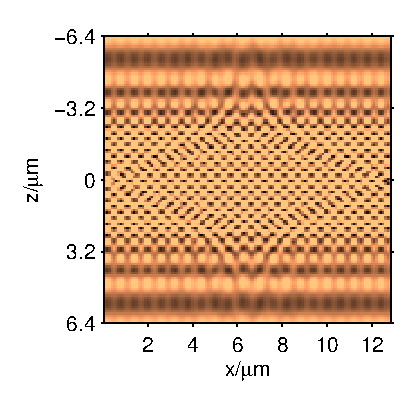
\includegraphics{../app_hilo/grating_xz}
  \caption{$xz-$cross section of the intensity distribution {\tt
      imgrat(:,64,:)} of the coherent image of the grating in sample
    space.}
  \label{fig:grating}
\end{figure}
The following listing shows how the sample object, i.e.\ the
fluorophore concentration, is generated.  The spherical shell is
calculated as the product of two Sinc functions in k-space and a
product with $r$ in real space. There is also a vertical line and a
rectangle. A slice through the simulated fluorophore concentration is
shown \figref{fig:input}~a). Note that the sphere is very faint but
it is the only of the three objects that is extended in $z$.

A shift by {\sf dz} in $z-$direction is done by multiplication with
$\exp(-ik{\sf dz})$ in k-space. This is only a good method to defocus
small distances {\sf dz} as the object will wrap around the borders.

\begin{lstlisting}
%% hollow sphere
kobj=sinc(rr(kpsf)./2).*sinc(rr(kpsf)./0.7); % in k-space
obj=rr(psf).*abs(ift(kobj)); % this is the sphere
maximum=max(obj);
obj(83:114,23:43,(sz*n)/2)=4*maximum; % rectangle in-focus rig ht top
obj(21:21,40:90,(sz*n)/2)=12*maximum; % in-focus line on the left
kobj=ft(obj); % shift the object a little bit in z
dz=1; % shift in pixels -> 1 equals 100nm
kobj=kobj.*exp(-i*2*pi*zz(kobj,'freq')*dz);
obj=ift(kobj);
\end{lstlisting}
In order to simulate the final image the fluorophore concentration is
multiplied by the excitation intensity distribution. The resulting
distribution of excited fluorophores is convolved with the simulated
detection point spread function (PSF) \nomenclature{PSF}{point spread
  function} \nomenclature{OTF}{optical transfer function} of the
microscope objective. The 3D convolution simulates the incoherent
image formation.
\begin{lstlisting}
%% detection PSF for imaging the fluorescence light
psf=kSimPSF({'lambdaEx',473;'lambdaEm',520;'na',1.4;'ri',1.518;...
        'sX',n;'sY',n;'sZ',sz*n;'scaleX',nmperpixel;...
        'scaleY',nmperpixel;'scaleZ',znmperpixel});
kpsf=ft(psf); % otf
fluo=obj.*imgrat; % excited fluorophores
strucflimg=ift(ft(fluo).*kpsf); % fluorescence image with 
                                % structured illumination
flimg=ift(ft(obj).*kpsf);       % wide field fluorescence image
%% extract focal planes
iu=real(squeeze(flimg(:,:,(sz*n)/2)));     % uniform illumination
in=real(squeeze(strucflimg(:,:,(sz*n)/2)));% structured illumination
\end{lstlisting}
The image $I_u$ for uniform illumination is shown in
\figref{fig:input}~b). \figref{fig:input}~c) depicts the image $I_n$
for non-uniform illumination with the \unit[600]{nm}-period grating.
\begin{figure}[!htb]
  \centering

  \subfigure[fluorophore distribution in the test object
  \textsf{obj}]{
\includegraphics[width=4cm]{../app_hilo/obj}}
  \subfigure[image under wide field illumination
  $I_u$]{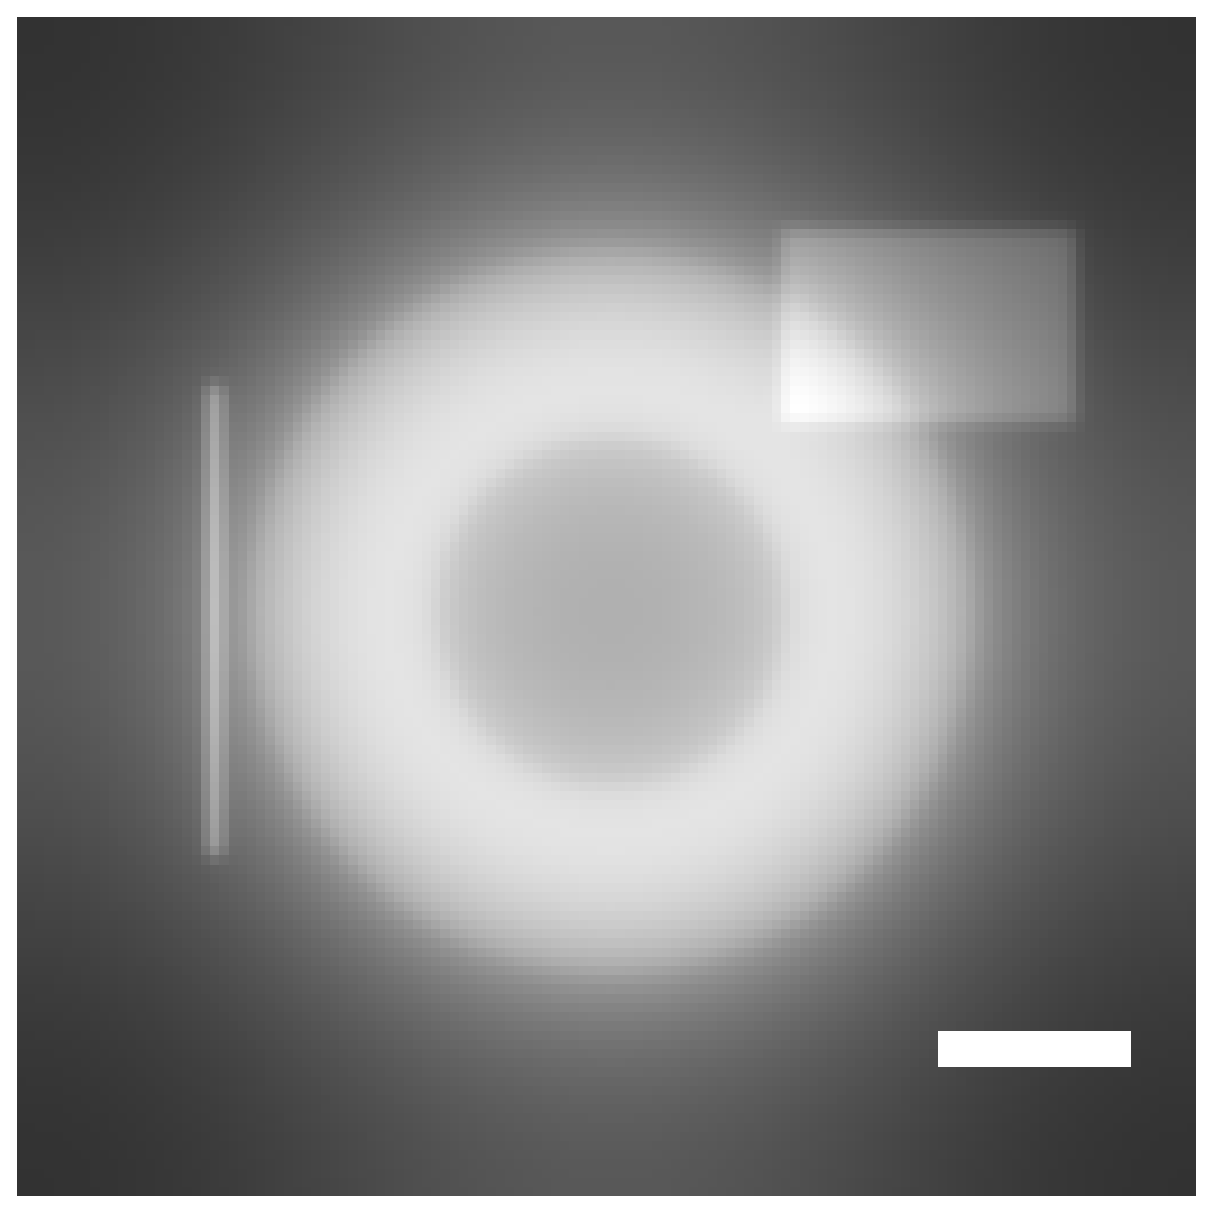
\includegraphics[width=4cm]{../app_hilo/iu}}
  \subfigure[image with structured illumination
  $I_n$]{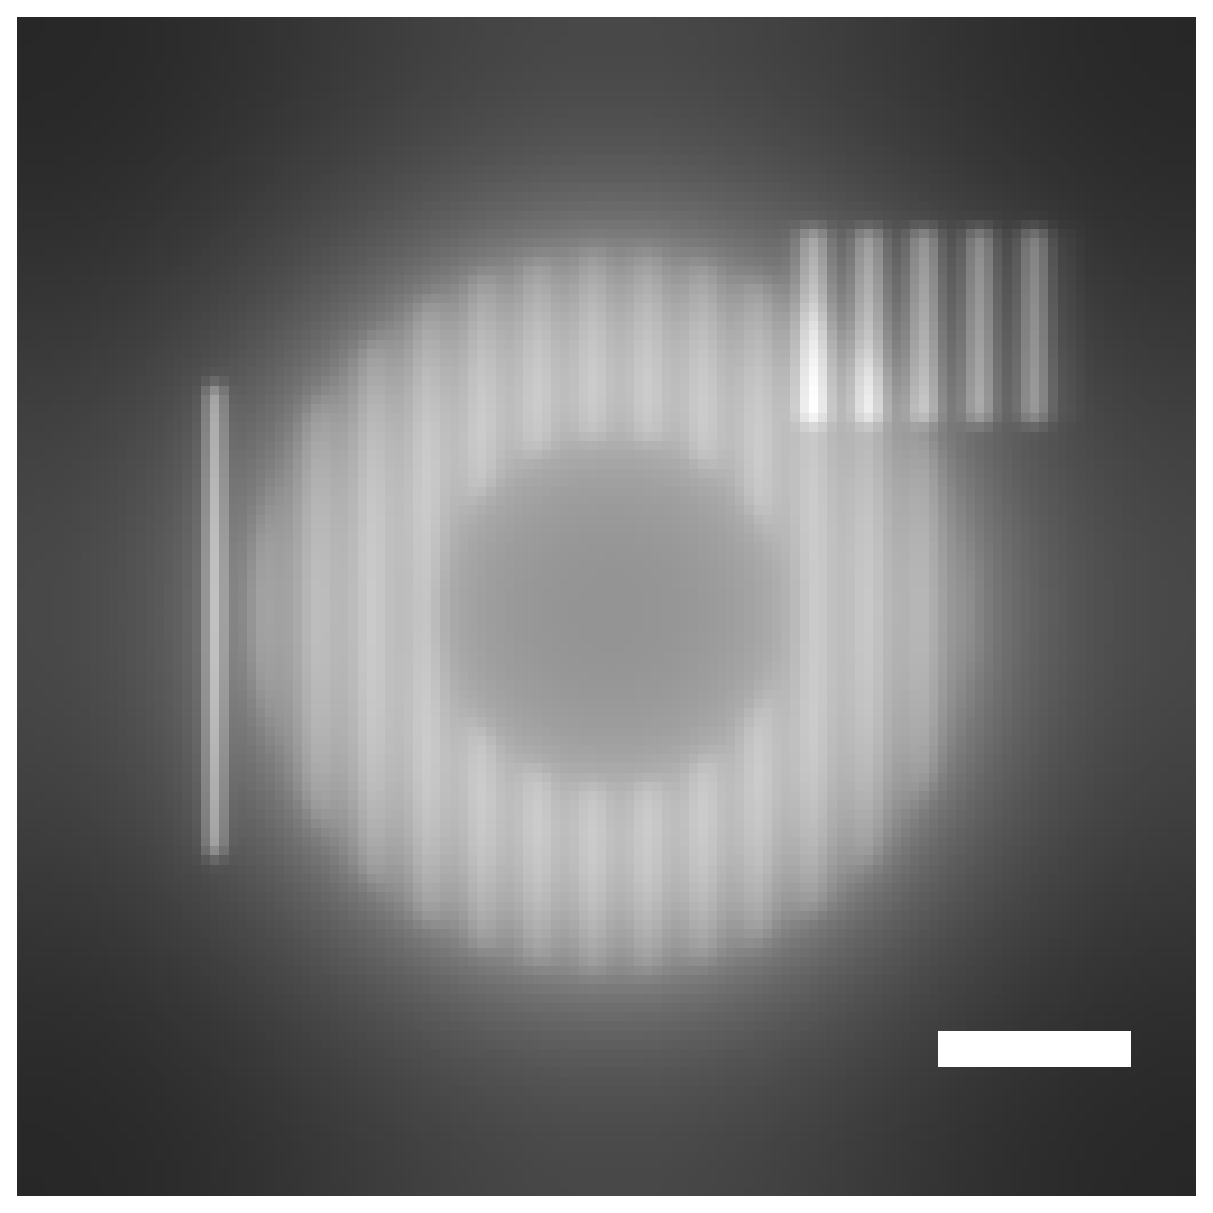
\includegraphics[width=4cm]{../app_hilo/in}}

  \caption{{\bf(a)} $xy-$slice of the object in the focal plane. It
    consists of a line, a spherical shell and a rectangle. Only the
    shell is extended in z. {\bf(b)} Image with wide field
    illumination. {\bf(c)} Image with structured illumination (grating
    period \unit[600]{nm}).  The scalebars are \unit[2]{$\mu$m}
    wide. }
  \label{fig:input}
\end{figure}
\figref{fig:defocus} shows the non-uniformly illuminated images for
different focus positions. The line and the rectangle both become
blurred and the contrast of the grating decreases in out-of-focus
planes. The grating in the sphere is still visible at approximately
the same contrast.
\begin{figure}[htb]
  \centering
  \subfigure[100 nm defocus]{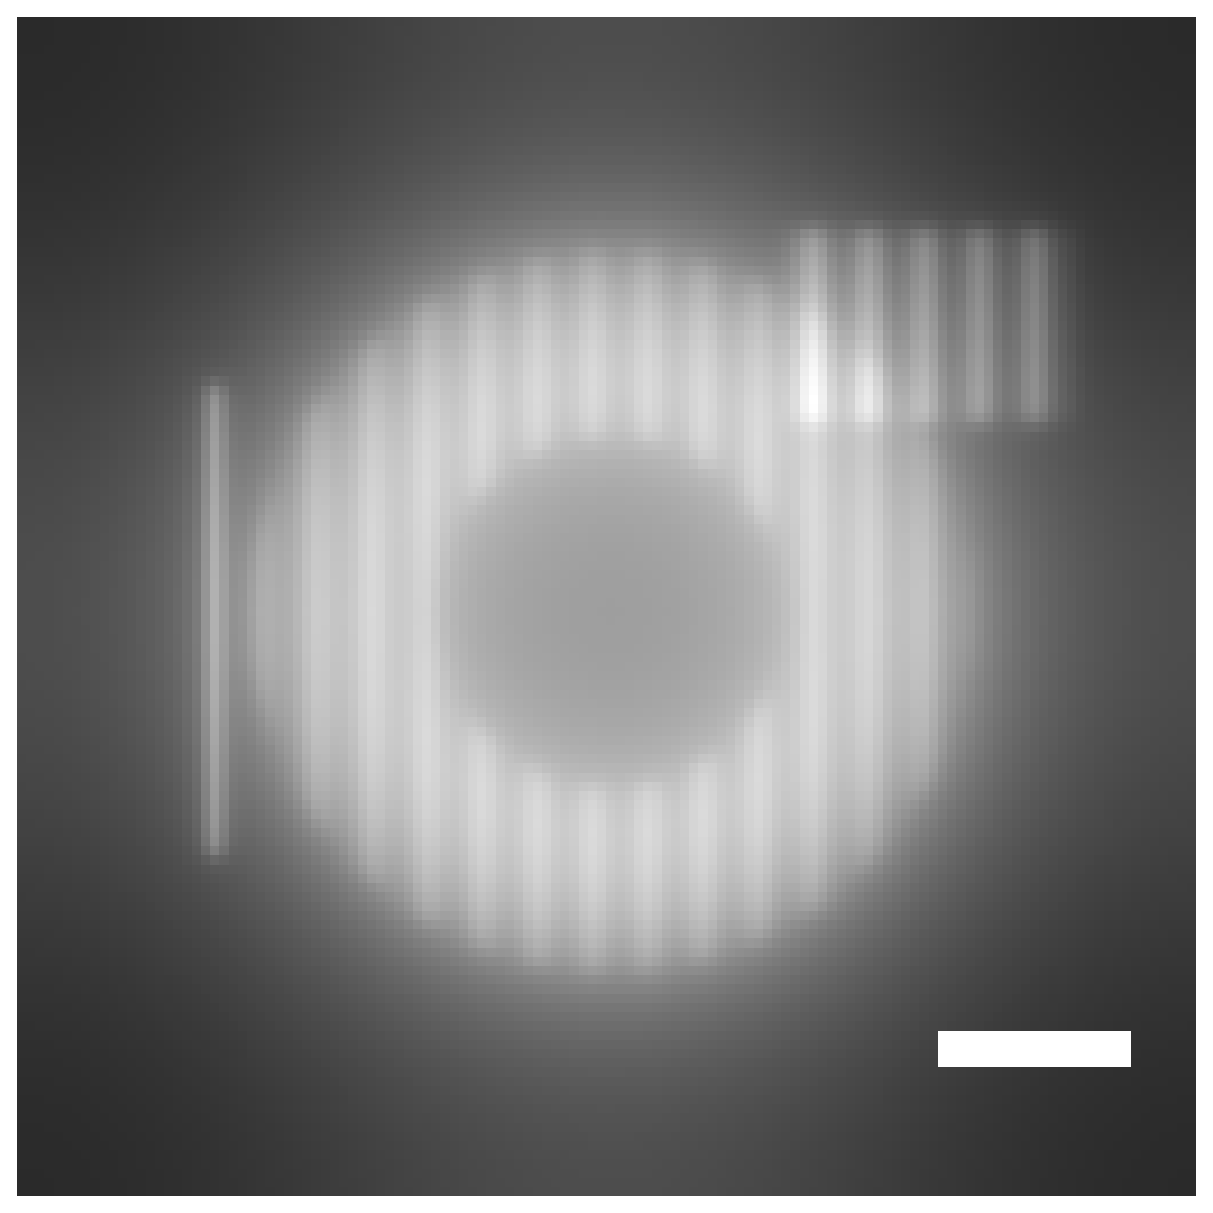
\includegraphics[width=4cm]{../app_hilo/in100}}
  \subfigure[200 nm]{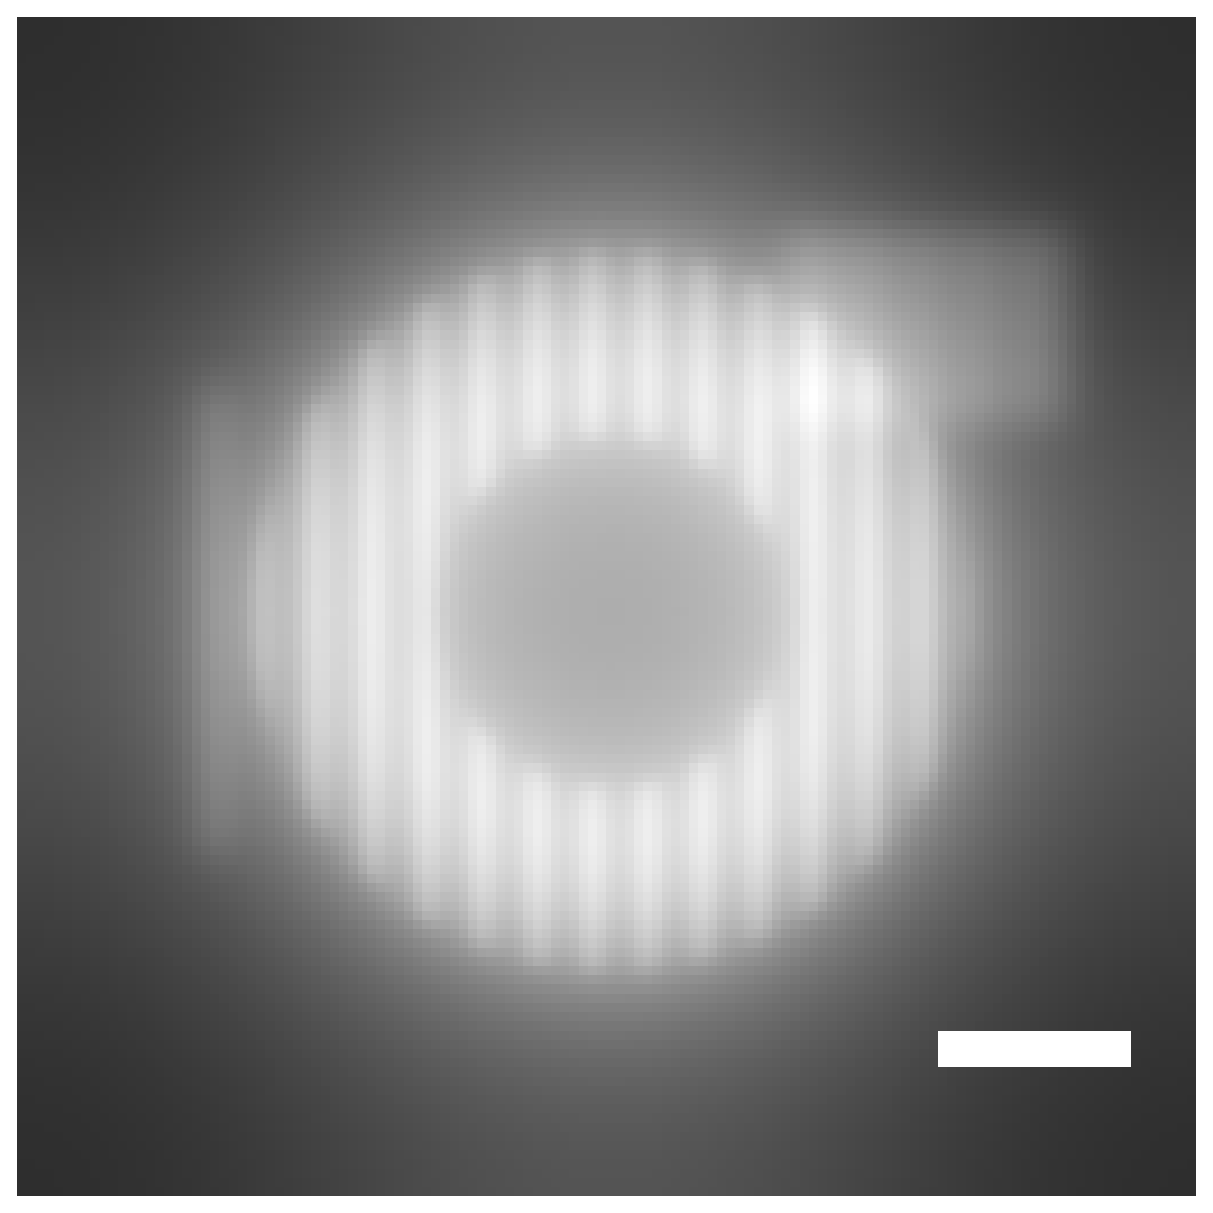
\includegraphics[width=4cm]{../app_hilo/in200}}
  \subfigure[500 nm]{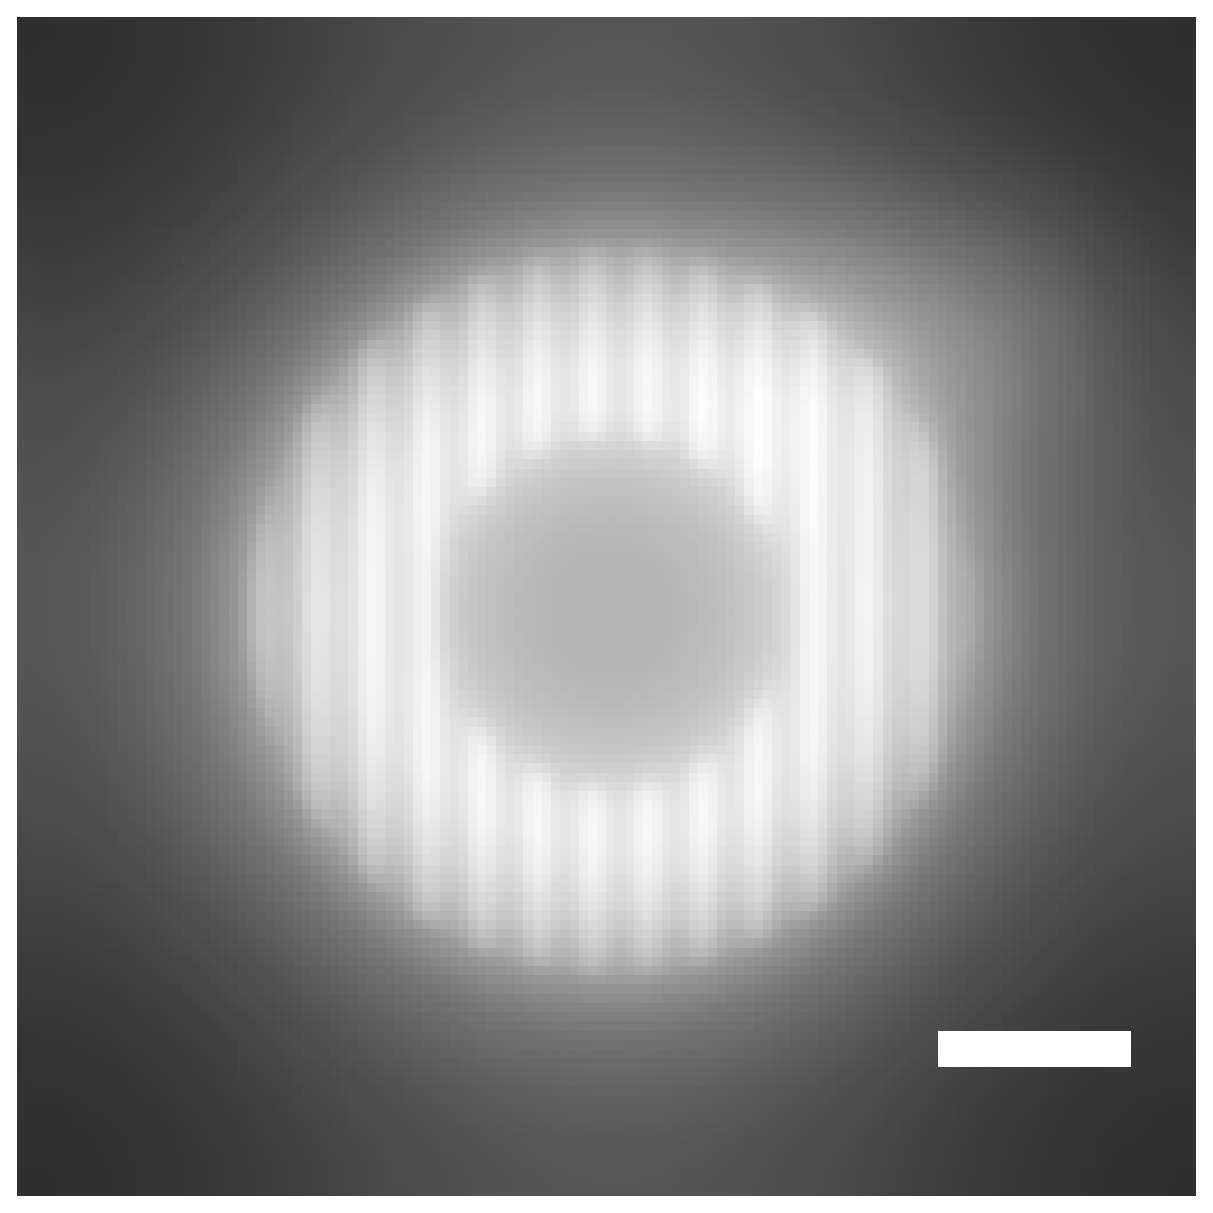
\includegraphics[width=4cm]{../app_hilo/in500}}
  \caption{Defocus series of the test object under structured coherent
    illumination (grating period \unit[600]{nm}). The scalebar is
    \unit[2]{$\mu$m} wide.}
  \label{fig:defocus}
\end{figure}
\section{Fundamentals of structured illumination}
If a fluorescent plane is imaged with a fluorescence wide field
microscope, the intensity of the image is constant no matter if the
plane is in focus or not (missing cone problem). 
\subsection{Apotome}
\label{sec:apotome}
Using non-uniform excitation light \cite{Neil1997} circumvent this
problem. They project a grid pattern into the sample using incoherent
illumination. For a fluorescent plane sample the modulation in the
image is highest, when the sample is in focus. If the plane is moved
out-of-focus, the modulation decreases. Hence it is possible to
achieve z-sectioning in a wide field microscope.

For one optically sectioned image $I_p$ they combine three grating
images $I_i$ (grating period
$1/\nu=\textrm{NA}/(\beta\lambda\tilde\nu)$, magnification $\beta$
between grating and specimen plane) with different phases:
\begin{align}
  I_p=\abs{I_1+I_2e^{i2\pi/3}+I_3e^{i4\pi/3}}
  \sim\left|2\frac{J_1(2u\tilde\nu(1-\tilde\nu/2))}{2u\tilde\nu(1-\tilde\nu/2)}\right|.
\end{align}

The last term is their result for the intensity of a fluorescent plane
with the defocus $u=8\pi z\sin^2(\alpha/2)/\lambda$. If no grating is
displayed ($\nu=0$) the resulting image $I_p$ is constant and the
microscope has no sectioning capability. A fine grating gives best
sectioning capability. However, there is also trade off to be made
because a fine grating will give very low contrast in a thick
specimen. Also for fine gratings a partially coherent illumination
should be used, so that orders are not cut off at the periphery of the
BFP \citetext{priv.\ comm.\ R.~Heintzmann}. This limits the field of
view for fine gratings.

For their reconstruction method it is necessary to capture three
images to compute one sectioned slice. This can be a problem if the
movement of the grating isn't perfect or if the object moves during
the exposures.
\subsection{HiLo}
This problem is addressed by \citet{2008Lim} and
\citet{2009Santos}. They describe an approach, for which only two
images need to be captured for each $z-$sectioned slice.  An image
with uniform illumination contains contributions of both in-focus and
out-of-focus fluorophores:
\begin{align}
\label{eqn:Iu}
  I_u(x,y)=I_\textrm{in}(x,y)+I_\textrm{out}(x,y).
\end{align}
The contribution from out-of-focus light $I_\textrm{out}$ is limited
to low spatial frequencies, i.e. $\tilde I_\textrm{out}(k_x,k_y)$ has
small support. The modulated part of the non-uniformly illuminated
image $I_n$ contains only information of the in-focus object
structure:
\begin{align}
\label{eqn:In}
  I_n(x,y)&=I_\textrm{in}(x,y)(1+M
  \sin(\kappa x+\varphi))+I_\textrm{out}(x,y),\\
  \kappa&=\frac{2\pi}{\lambda}n\sin(\alpha)\nu.
\end{align}
We can recover the sectioned image as a combination of high-frequency
components of the wide field image $I_u$ and the low-frequency
components of the modulated part of the non-uniform image $I_n$.
\subsubsection{Using speckle pattern as non-uniform illumination (local variance estimation)}
In the older publication \citep{2008Lim} a random speckle pattern is
projected into the sample. For comparison with the other methods we
describe a reimplementation of their method.

In order to process the non-uniform image it is divided into
subregions.  As a measure of local contrast in each of these
subregions the relative standard deviation $c$ is calculated (the
operator $\avg{\cdot}$ indicates averaging over a pixel
neighbourhood):
\begin{align}
  c_n=\frac{\sqrt{\avg{I_n^2}-\avg{I_n}^2}}{\avg{I_n}}.
\end{align}
The relative standard deviation $c_n$ will be zero for image regions
without in-focus contributions. Its value increases as the modulation
of the non-uniform illumination increases (that's what we
want). However $c_n$ also increases if there is a small in-focus
feature. In that we are not interested as we only want to build up an
image of in-focus fluorophores with low spatial frequencies. 

The authors state that a corrected relative standard deviation $c_s$
of the non-uniform illumination can be obtained by removing the
standard deviation
$c_0=\frac{\sqrt{\avg{I_u^2}-\avg{I_u}^2}}{\avg{I_u}}$ of the
wide field image:
\begin{align} 
  c_s^2=\frac{c_n^2-c_0^2}{1+c_0^2}
  =
  \frac{\avg{I_n^2}}{\avg{I_n}^2}
  \frac{\avg{I_u^2}}{\avg{I_u}^2}-1.
\end{align}
The product $I_{su}=c_s\avg{I_u}$ then provides a low resolution
version of $I_u$ that is optically sectioned (using information from
$I_n$) even for the DC frequency.

The following listing shows how this algorithm can be applied to two
input images {\sf iu} and {\sf in}. Instead of doing a discrete
integration over regions we multiply with a Gaussian in Fourier
space. The cutoff frequency $k_c$ of the filter is chosen low enough
so that $c_s$ doesn't contain any structure of the grating anymore.
\begin{lstlisting}
si=size(in);   n=si(1);  % only square images
kc=0.04;                 % filter cutoff
r=rr(in,'freq');
klp=exp(-r.^2/(2*kc^2)); % low pass
khp=1-klp;               % high pass
ina=ift(ft(in).*klp);
in2a=ift(ft(in.^2).*klp);
iua=ift(ft(iu).*klp);
iu2a=ift(ft(iu.^2).*klp);
cs2=in2a.*iua.^2./(ina.^2.*iu2a)-1;
isu=sqrt(cs2).*iua;      % sectioned version of iu
kihp=ft(iu).*khp;
kilp=ft(isu).*klp;
\end{lstlisting}
\begin{figure}[htb]
  \centering
  \subfigure[Corrected relative standard deviation $c_s$.]{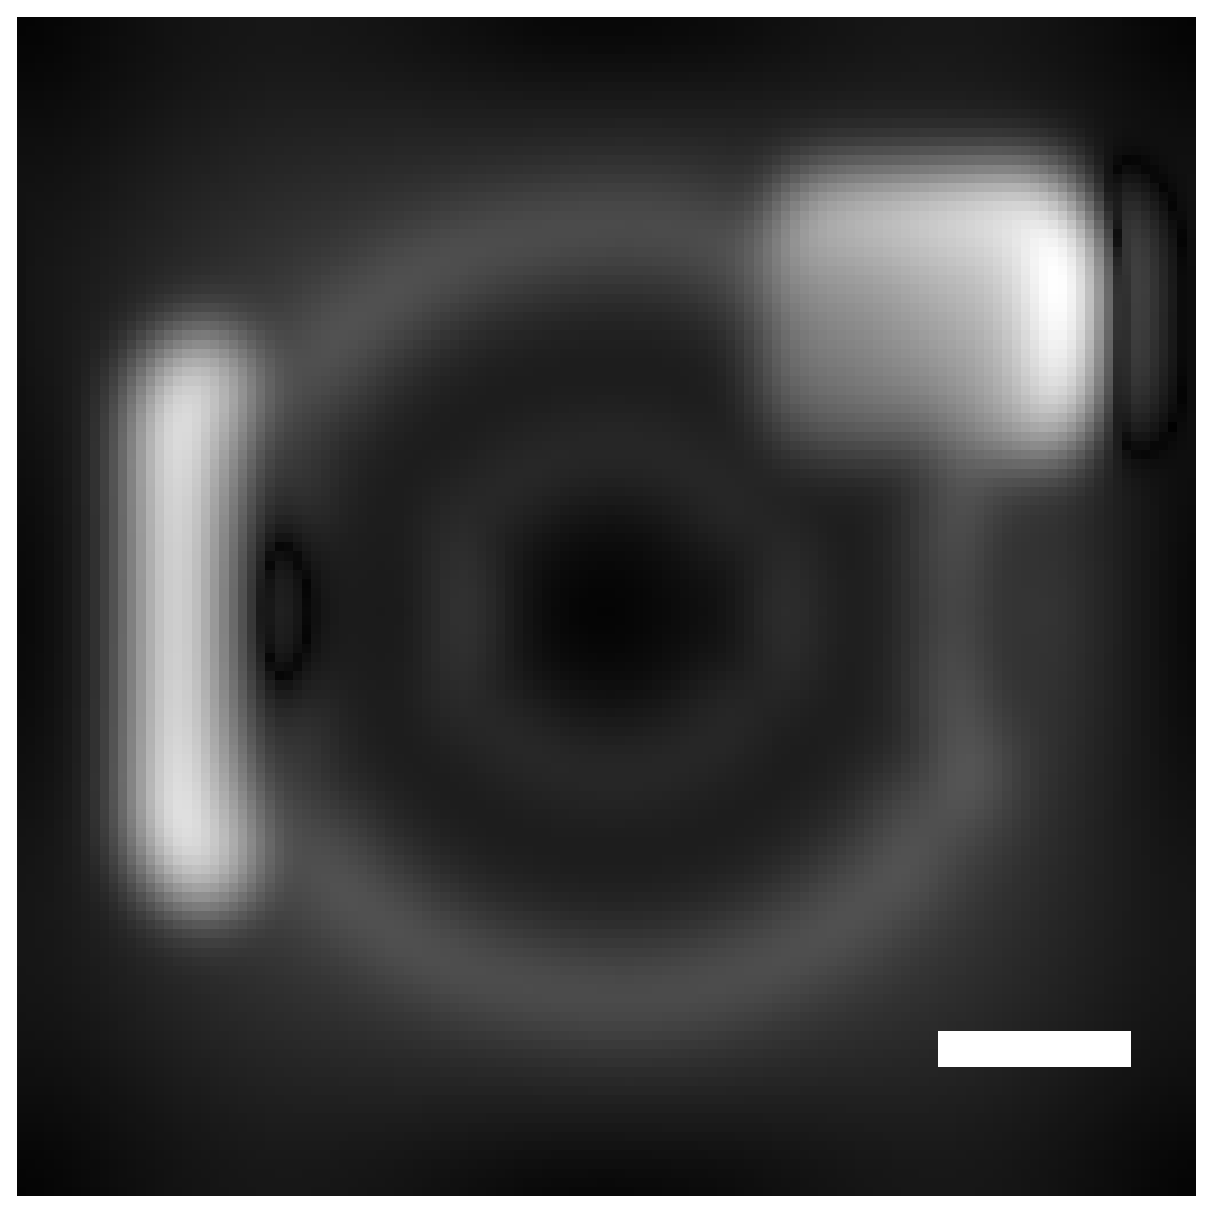
\includegraphics[width=4cm]{../app_hilo/cs}}
  \subfigure[The product $I_{su}=c_sI_u$]{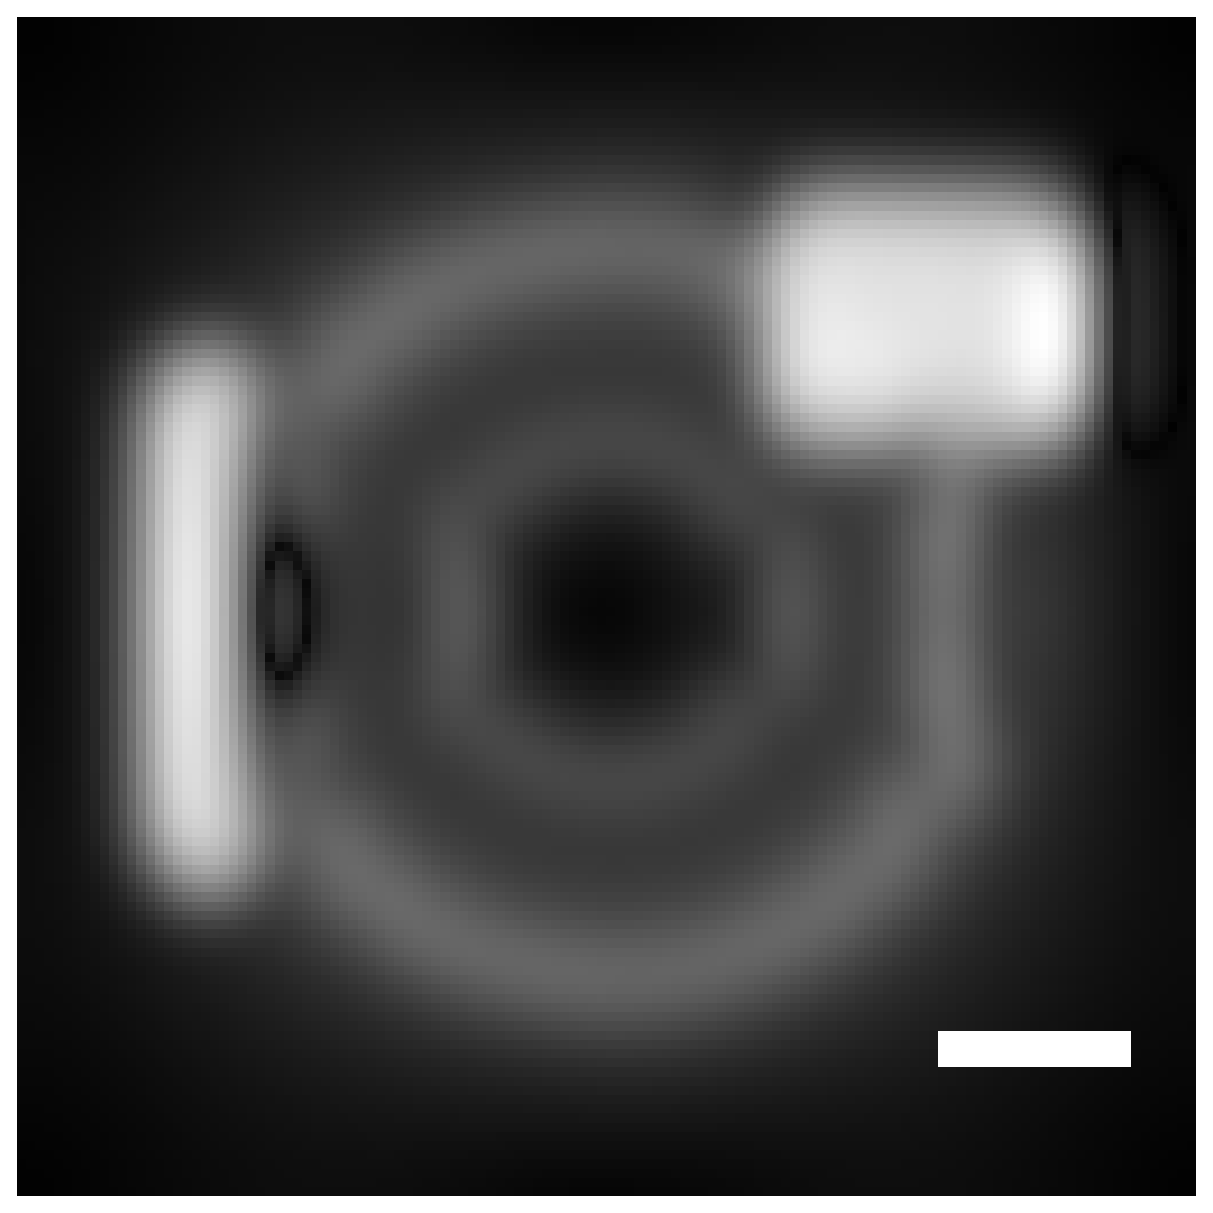
\includegraphics[width=4cm]{../app_hilo/isu}}
  \subfigure[Low spatial frequency section $I_\textrm{lp}$]{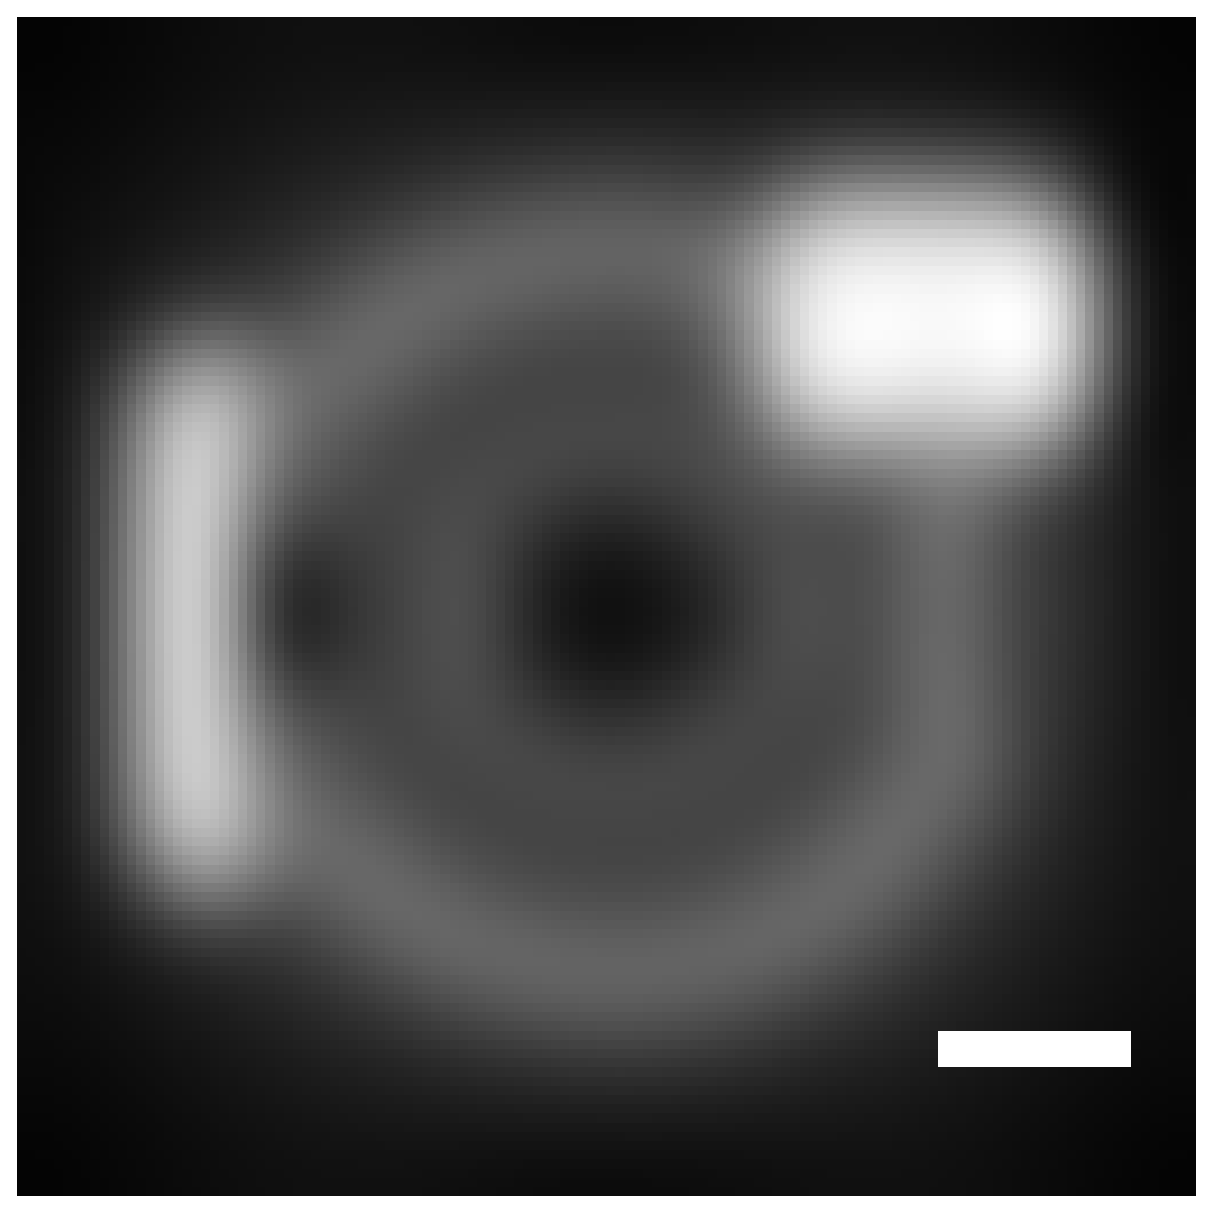
\includegraphics[width=4cm]{../app_hilo/ilp}}
  \caption{Several intermediate results of the algorithm. The scalebar is
    \unit[2]{$\mu$m} wide.}
  \label{fig:hilo1interm}
\end{figure}
The HiLo method combines a low-pass filtered version of $I_{su}$ with
a high pass filtered version of the uniformly illuminated image $I_u$.
To do this the two images are scaled for a seamless interface along
the circle $K$ with radius $\abs{\vect k_c}$ in k-space and then added:
\begin{align}
  \eta=\!\!\!\!\ointop_{\partial K_{k_c}}\!\!\!
  \frac{\abs{I_\textrm{hp}}}{\abs{I_\textrm{lp}}}\,\textrm{d}\vect k,\\
  I_\textrm{hilo}=\eta I_\textrm{lp}+I_\textrm{hp}.
\end{align}

This is done in the following listing:
\begin{lstlisting}
ring=real(ft(besselj(0,2*pi*kc*n.*r)));
ring2=r-1./n<kc & r+1./n>kc;
cring=ring.*ring2;
nring=cring./sum(cring); % normalized ring with radius kc
eta=sum(abs(kihp)./abs(kilp).*nring);
ihilo=ift(eta.*kilp+kihp);
\end{lstlisting}

\begin{figure}[htb]
  \centering
  \subfigure[High frequency components $I_\textrm{hp}$ of wide field.]{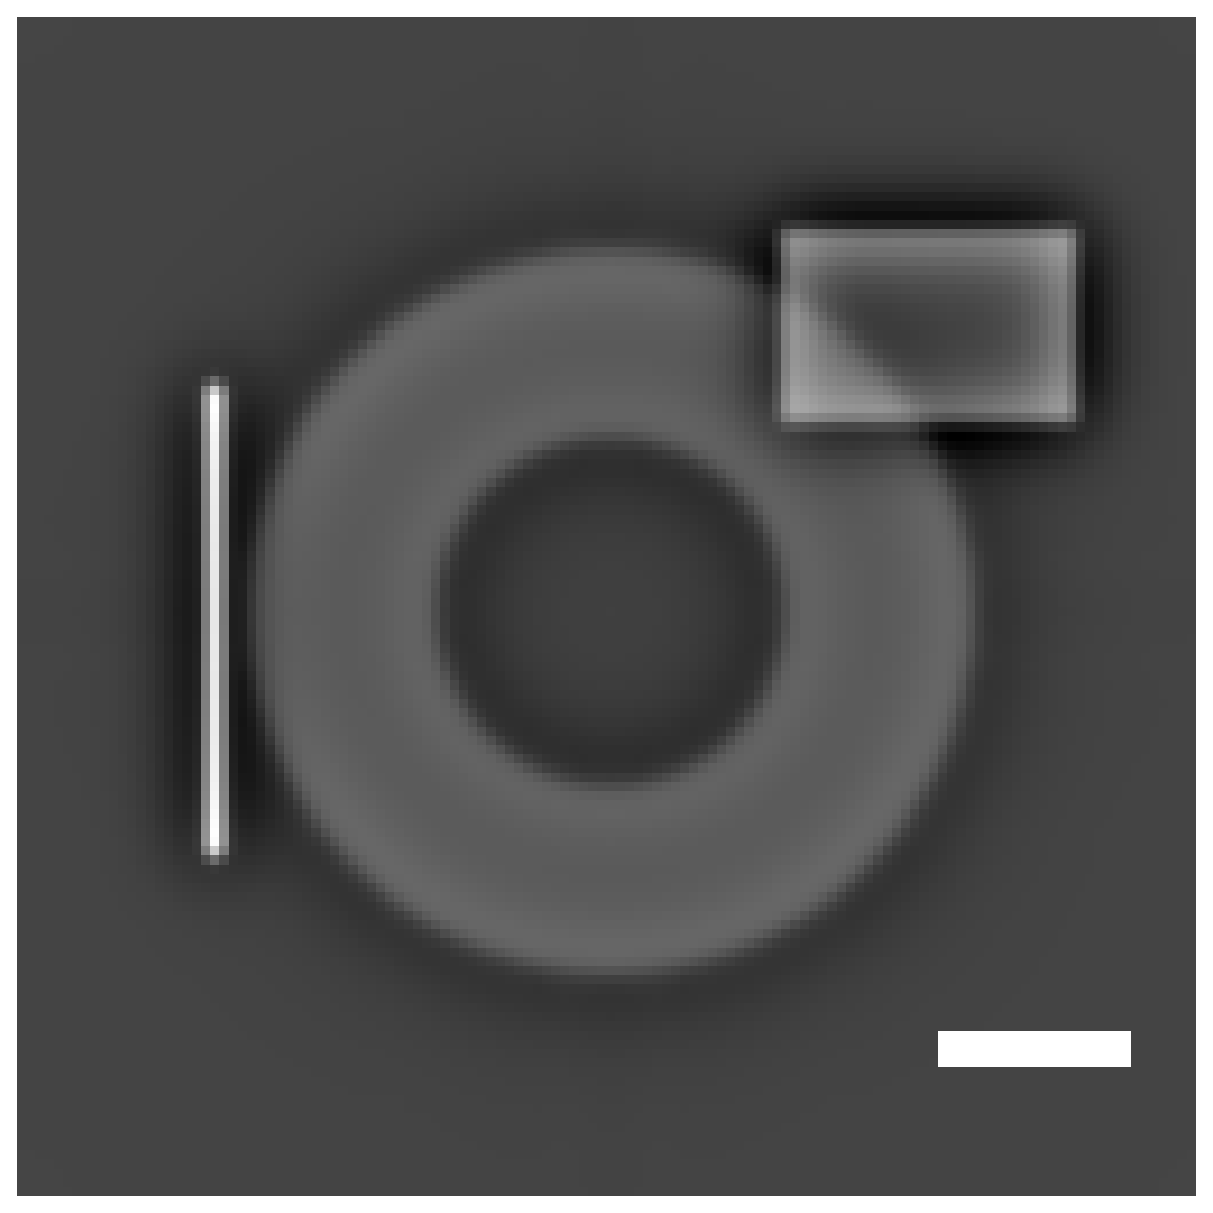
\includegraphics[width=4cm]{../app_hilo/ihp}}
  \subfigure[Combined images $\tilde I_\textrm{hilo}$ in k-space.]{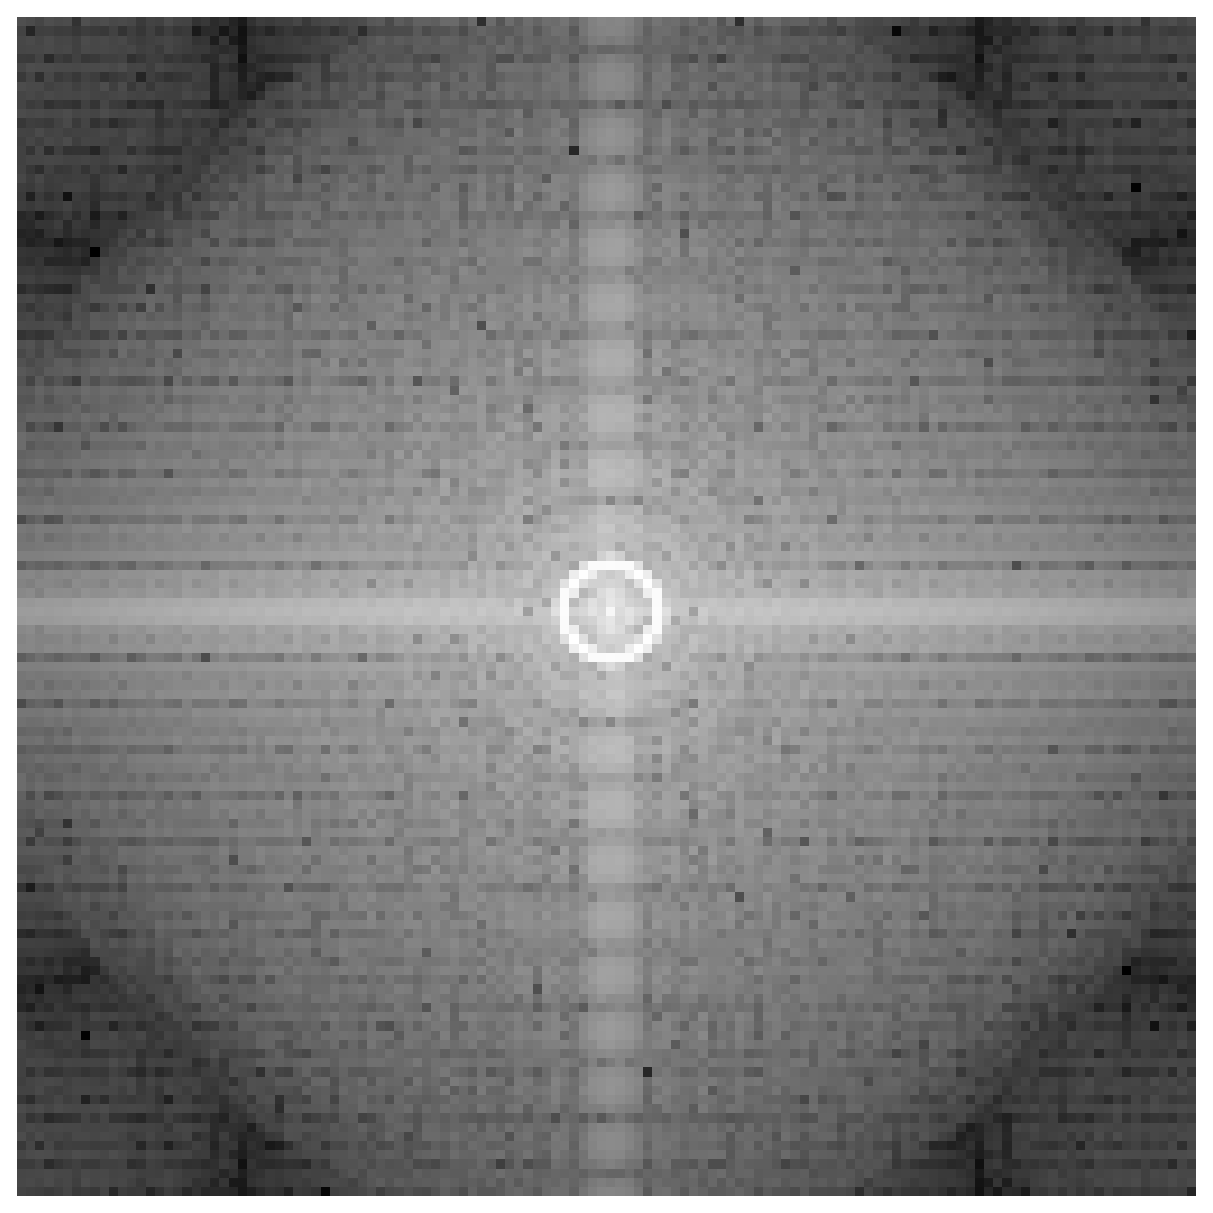
\includegraphics[width=4cm]{../app_hilo/kihilo}}
  \subfigure[Combined section $I_\textrm{hilo}$.]{\label{fig:ihilo}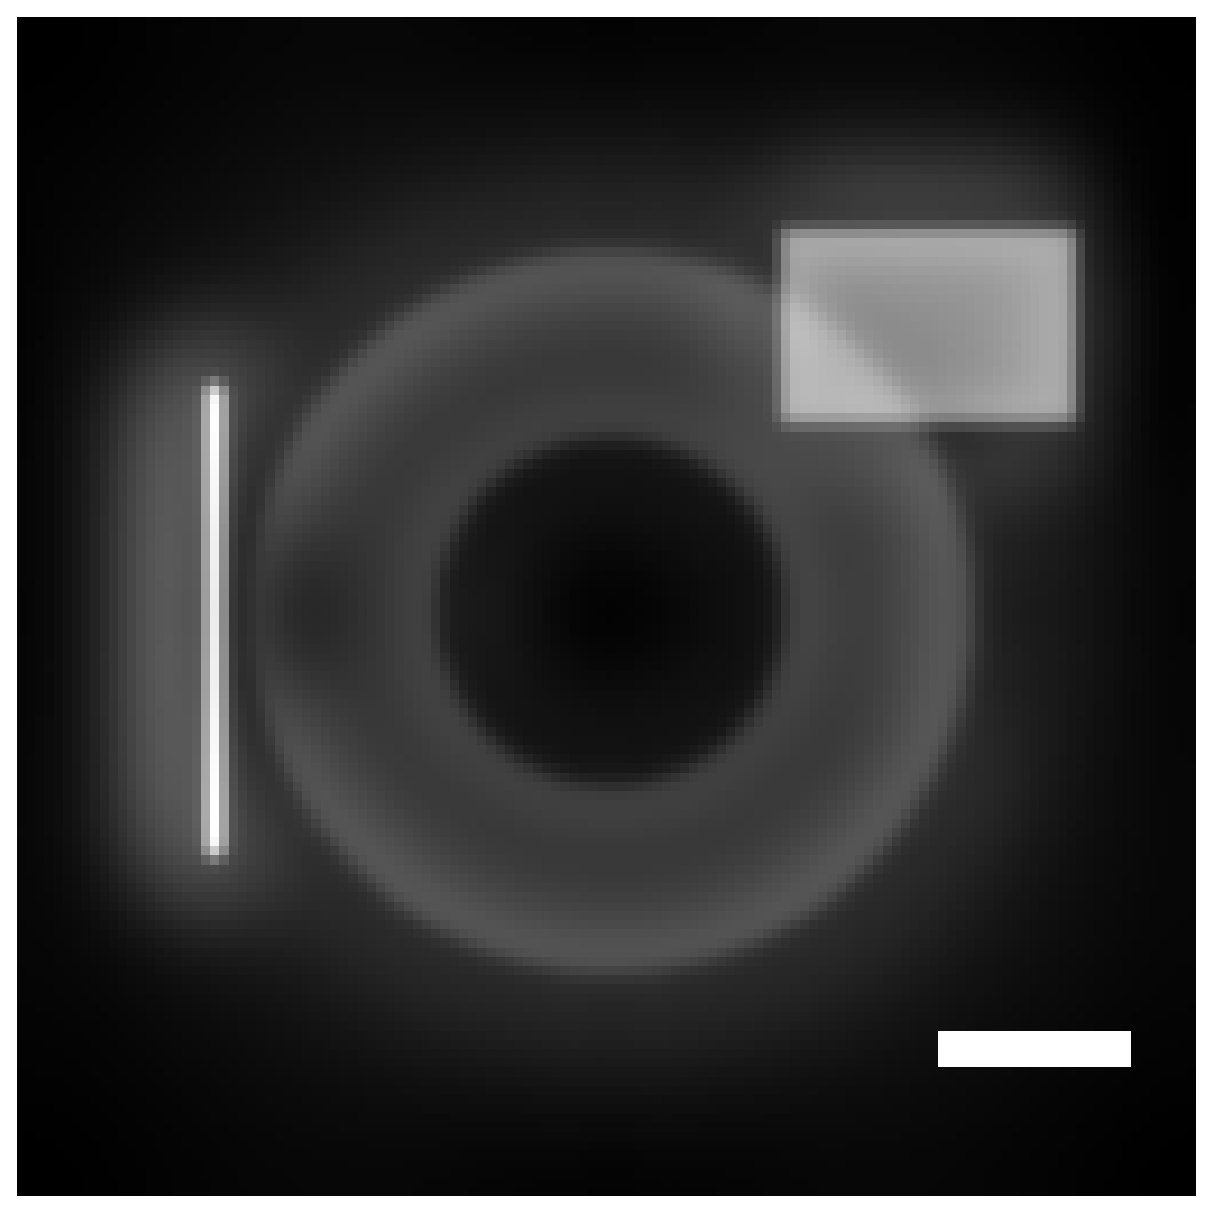
\includegraphics[width=4cm]{../app_hilo/ihilo}}
  \caption{More intermediate and the end result of the HiLo local
    variance estimation algorithm. The white circle in image {\bf (b)}
    marks the cutoff frequency $k_c$ of the spatial low pass
    filter. The scalebars are \unit[2]{$\mu$m} wide.}
  \label{fig:hilo1interm2}
\end{figure}

\subsubsection*{Discussion}
This algorithm only requires the illumination intensity in $I_n$ to
fluctuate over a certain region and one uniform image. The
reconstructed results somewhat resemble a sectioned image. The main
advantage is that all the filtering could have been done in real
space, without ever doing any Fourier transform.
\subsubsection{Reconstructing the sample illuminated with a grating
  pattern (single side-band demodulation)}
The more recent paper \cite{2009Santos} uses a more defined pattern in
the excitation illumination than random speckle. A grating is
projected into the specimen using a spatial light modulator.

Starting from a wide field image $I_u$ and an image $I_n$ that has been
illuminated with a grating they first determine the ratio $R=I_n/I_u$.
With equations \eqref{eqn:Iu} and \eqref{eqn:In} defining the
relationship between in-focus and out-of-focus light in both images
they obtain:
\begin{align}
  R&=1+CM\sin(\kappa x+\varphi)),\\
  C&=\frac{I_\textrm{in}}{I_\textrm{in}-I_\textrm{out}}.
\end{align}
Here $C$ is the local image contrast (containing information similar
to $c_s$ in the HiLo local variance method) that is necessary to
determine the low-resolution sectioned image. The Fourier transform
$\tilde R$ (see \figref{fig:hatR}) of the ratio contains a peak in the
centre (due to the constant 1). Then there are strong $\pm 1$ orders
and weaker $\pm 2$ orders because a rectangular grating is imaged into
the sample. If only a Sine grating was imaged into the sample, only the $\pm 1$ orders would be present.
%FIXME the weak grating isn't in In! so maybe it is due to the ratio

To extract the modulated signal from $R$, a filter is constructed that
selects only the first order on the right side of the Fourier
transform $\tilde R$. The result of the filter is shown in
\figref{fig:hatR+}. The intermediate image $I_{su}=\abs{R^+}I_u$ (see
\figref{fig:isu2}) contains the low-resolution sectioned image.

\begin{figure}[htb]
  \centering \subfigure[Ratio
  $R=I_n/I_u$.]{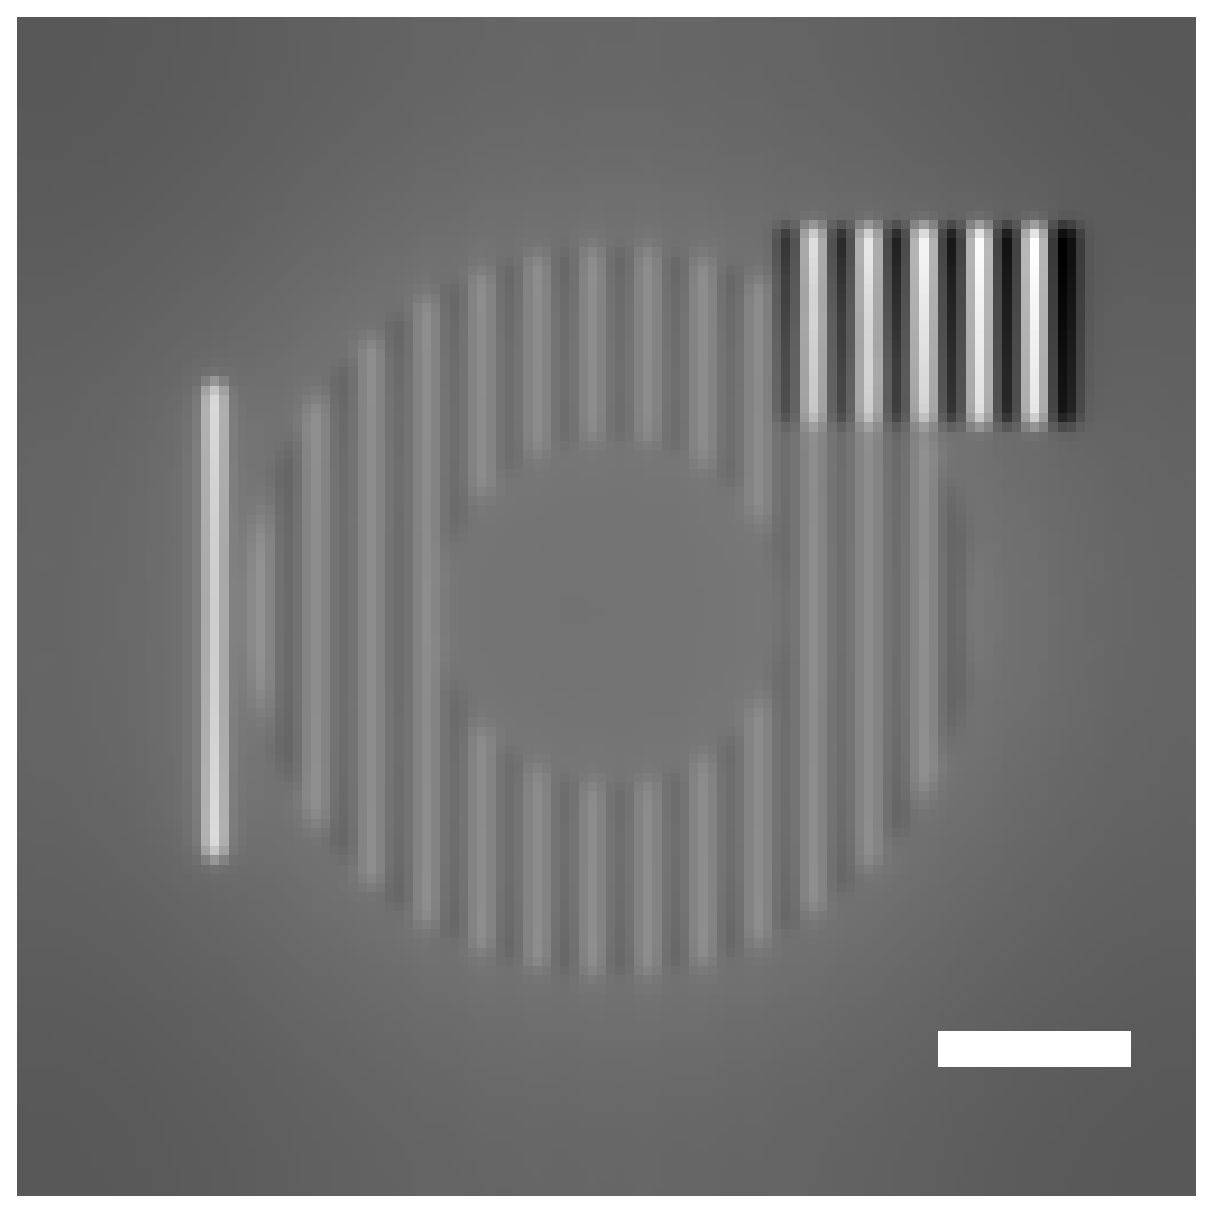
\includegraphics[width=4cm]{../app_hilo/ratio}}
  \subfigure[Fourier transform $\tilde
  R$.]{\label{fig:hatR}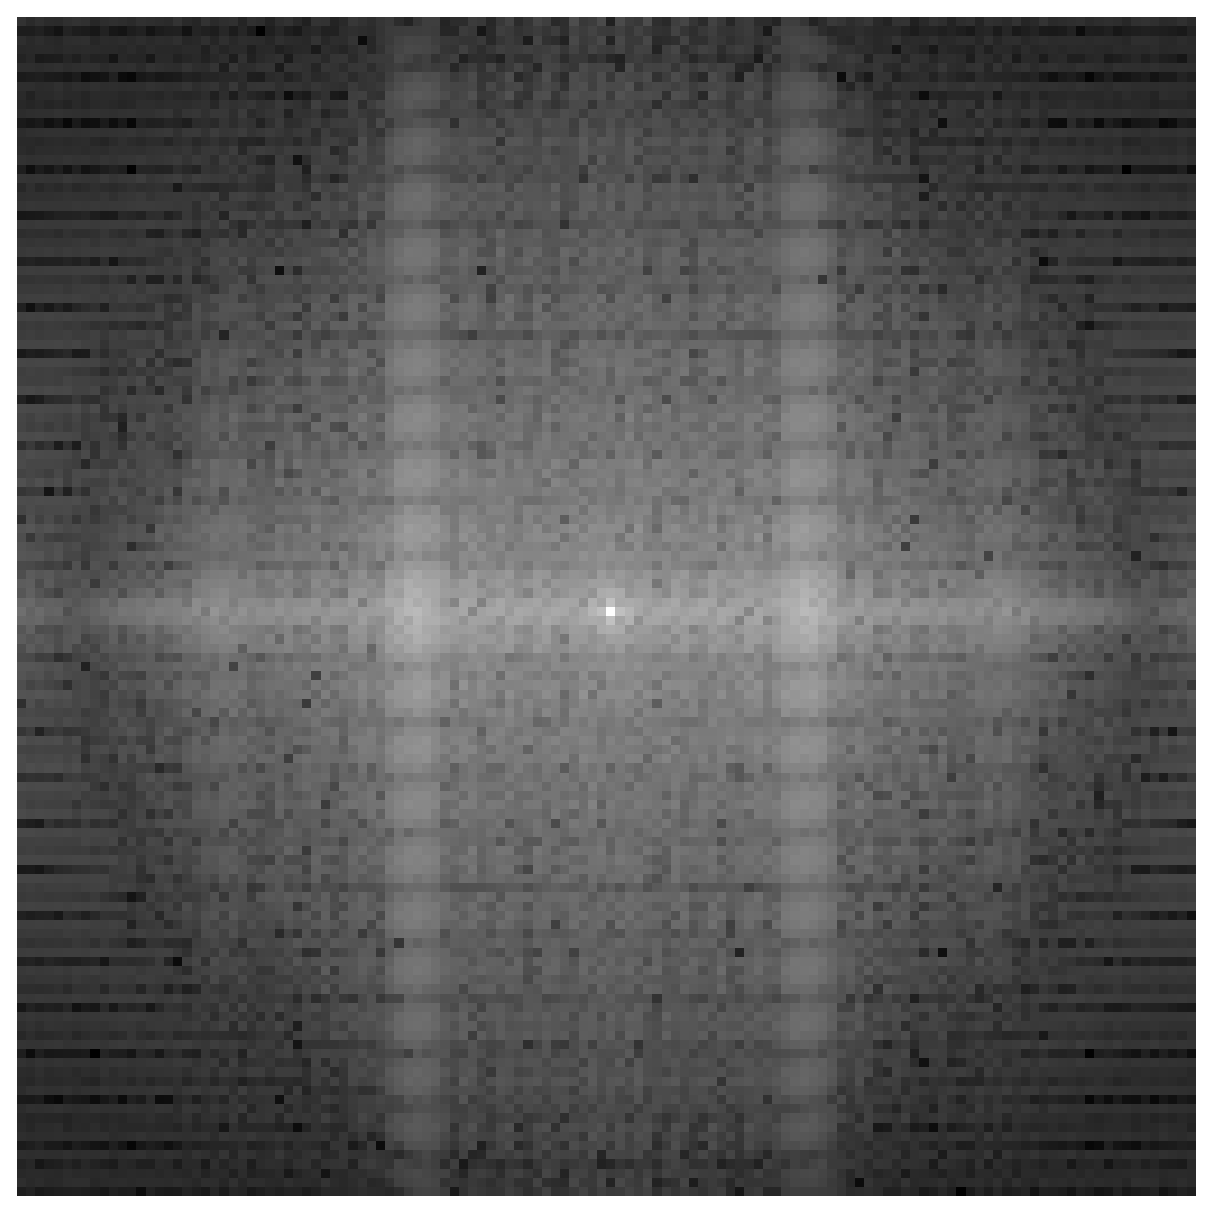
\includegraphics[width=4cm]{../app_hilo/ftratio}}
  \subfigure[Filtered first order $\tilde
  R^+$.]{\label{fig:hatR+}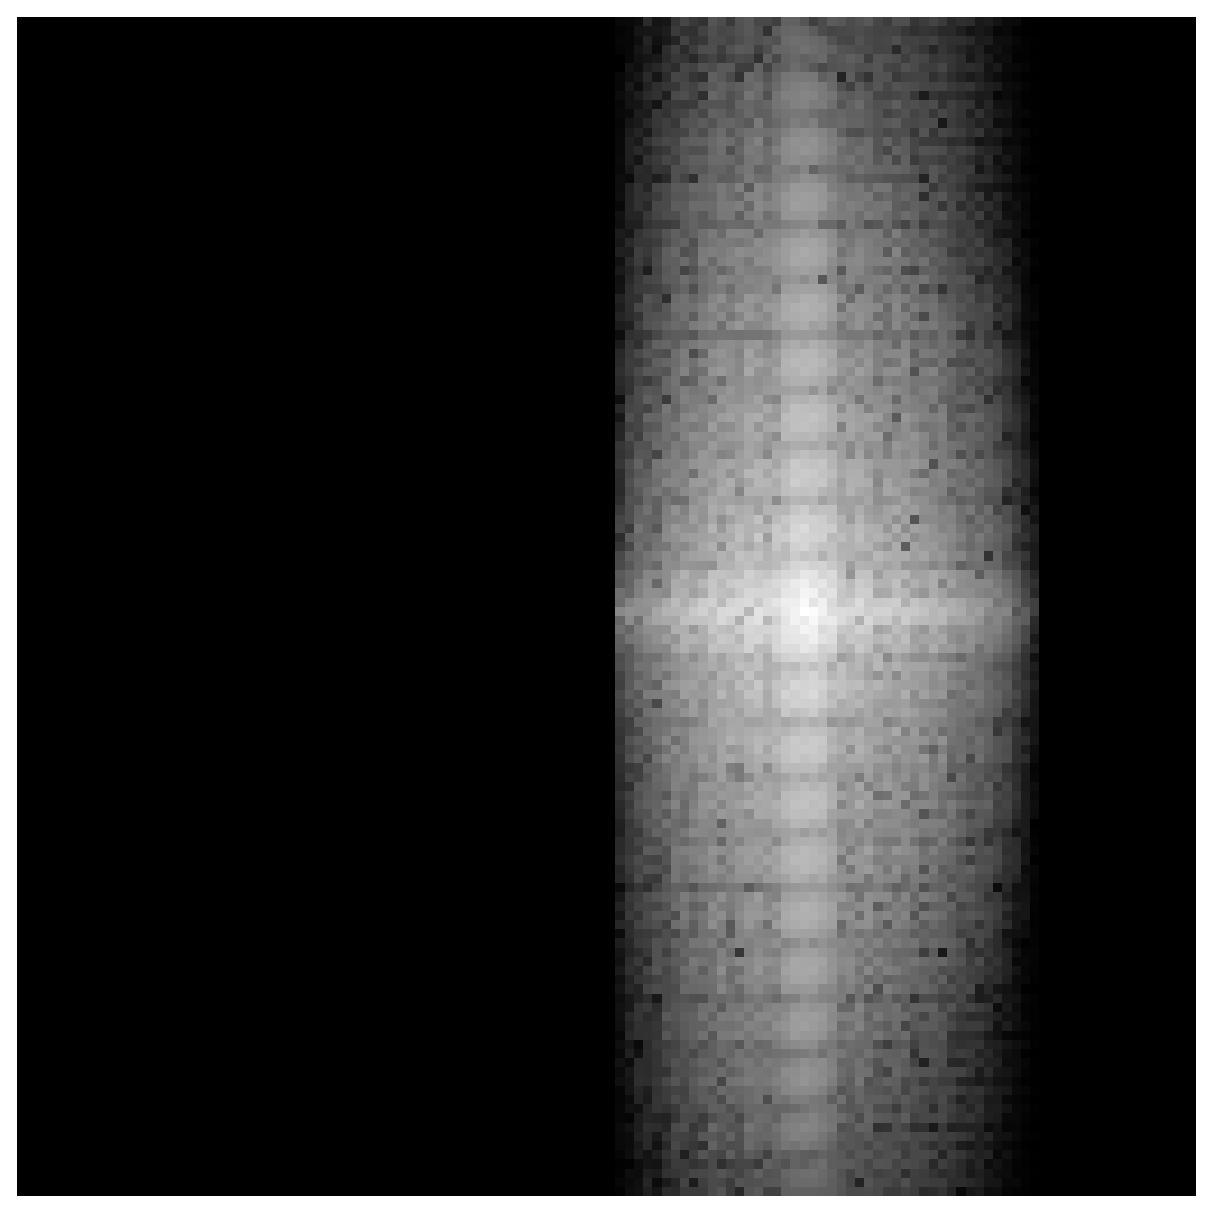
\includegraphics[width=4cm]{../app_hilo/filterftratio}}
  \caption{Intermediate results for the HiLo single side-band
    demodulation algorithm. The scalebar in (a) is \unit[2]{$\mu$m}
    wide.}
  \label{fig:hilo2}
\end{figure}

The following listing shows the code for the algorithm:
\begin{lstlisting}
si=size(in);   n=si(1);   r=rr(in,'freq');
ratio=in./iu;
%% select R+ and construct isu
filter=gaussf((xx(in,'freq')>0.1) & (xx(in,'freq')<0.27),4);
ftratio=ft(ratio);
cm=abs(ift(filter.*ftratio));
isu=cm.*iu
kc=.07;          % calculate low pass filtered low-res section
klp=exp(-r.^2/(2*kc^2));
ilp=real(ift(klp.*ft(isu)))
% calculate high pass filtered high-res section
ihp=real(ift((1-klp).*ft(iu)))
% construct the circle for integration in k-space
ring=abs(ft(besselj(0,2*pi*kc*n.*r)));
ring2=r-1./n<kc & r+1./n>kc;
cring=ring.*ring2;
nring=cring./sum(abs(cring))
eta=sum(abs(ft(ihp))/abs(ft(ilp)).*nring) % integrate along circle
ihilo=eta.*ilp+ihp                        % combined section
\end{lstlisting}
We chose the cutoff frequency $k_c$ high enough so that the low
resolution sectioned image $I_\textrm{lp}$ (computed from uniform
image) doesn't look too smooth but also low enough so that not too
much information is lost from the high resolution sectioned image
$I_\textrm{hp}$ image (computed from modulated image). The scale
factor $\eta$ for $I_\textrm{lp}$ and $I_\textrm{hp}$ is calculated as
in the previous section. Finally the combined sectioned image is
displayed in \figref{fig:ihilo2}.
\begin{figure}[htb]
  \centering
  \subfigure[$I_{su}$]{\label{fig:isu2}
\includegraphics[width=4cm]{../app_hilo/isu2}}
  \subfigure[$I_\textrm{lp}$]{
\includegraphics[width=4cm]{../app_hilo/ilp2}}
  \subfigure[$I_\textrm{hilo}$]{\label{fig:ihilo2}
\includegraphics[width=4cm]{../app_hilo/ihilo2}}
  \caption{Intermediate results and the end result for the HiLo single
    side-band demodulation algorithm. The scalebars are
    \unit[2]{$\mu$m} wide.}
  \label{fig:hilo2_2}
\end{figure}
\subsubsection*{Discussion}
One advantage of the single side-band demodulation method compared to
the local variance estimation method is that it allows for a higher
cut-off frequency $k_c$ without introducing artifacts in the
intermediate image $I_{su}$. That accounts for the better appearance
of the result \figref{fig:ihilo2} compared to \figref{fig:ihilo} (at
least for this particular grating).

Probably the results would be even better, if a Sine pattern was
illuminated into the sample. Then, there would be no second orders in
\figref{fig:hilo2}~(b) and the filter would be easier to place.

Calculation of the ratio (single side-band demodulation) isn't the
only way to extract the modulated signal. Another approach involving
subtracting the wide field image\footnote{Suggested by R.~Heintzmann.}
and shifting in Fourier space is discussed in the following section.
\section{Alternative method (subtraction method)}
Instead of using a non-hermitian filter to extract the modulated part
of the non-uniformly illuminated image $I_n$ it is also possible to
employ the Fourier shift theorem: A shift in real space is 
a multiplication with a phase factor in k-space. 

Given two images in real space $f(\vect x)$ and $g(\vect x)$. The
image $g$ contains the same information as $f$ but shifted by a vector
$\vect a$. The theorem can be expressed like this:
\begin{align}
  g(\vect x)=f(\vect x+\vect a)
  \quad
  \rightarrow
  \quad
  \tilde g(\vect k)=e^{i\vect k\vect a}\tilde f(\vect k).
\end{align}
One can find the shift by searching for the maximum $\vect x_0=\vect a$ in
the cross-correlation $cov(\vect x)$:
\begin{align}
  cov(f,g)(\vect x)
  =\int f(\vect\chi) g(\vect x+\vect\chi) \textrm{d}\vect\chi
  =f(\vect x)\otimes g(-\vect x)
  =FT^{-1}(\tilde f(\vect k)\cdot\tilde g^*(\vect k)).
\end{align}
First the uniform image $I_u$ is subtracted from the image with the
grating $I_n$ in order to suppress the zero order. The following code
integrates over a circle around the origin in k-space to find a
constant {\sf kappa} to scale $I_u$ with. Furthermore the
Fourier transform of the images is divided by the OTF in order to
correct for the non-constant frequency transfer in the microscope
objective\footnote{Note that for this to work with noisy data a
  Wiener filter would be necessary.}
\begin{lstlisting}
kin=ft(in);
kiu=ft(iu);
% scale kin and kiu so that ic has no zero order
kappa=sum(abs(kin)./abs(kiu).*(rr(in)<5))./sum(rr(in)<5)
%% project otf along z
skpsf=squeeze(sum(kpsf,[],3));
corr=gaussf((rr(skpsf,'freq')<.42),3)./skpsf;
%% correct for the otf
ckin=corr.*kin;
ckiu=corr.*kiu;
%% correlate to find grating positions
ackin=abs(ckin-kappa.*ckiu);
ackiu=abs(ckiu).*(rr(ackiu,'freq')<.16 | abs(xx(ackiu,'freq'))<.06);
\end{lstlisting}
The Fourier transform of the OTF-corrected non-uniform image is shown
in \figref{fig:ackin}. It still contains the $\pm1$ orders. In order
to measure their exact position (depending on the grating period {\sf
  P}) the zero order of the wide field k-space is selected (in variable
{\sf ackiu}, \figref{fig:hilo3}~(b)) and cross-correlated with {\sf
  ackin} (\figref{fig:hilo3}~(a)).

\begin{figure}[htb]
  \centering \subfigure[{\sf
    ackin}]{\label{fig:ackin}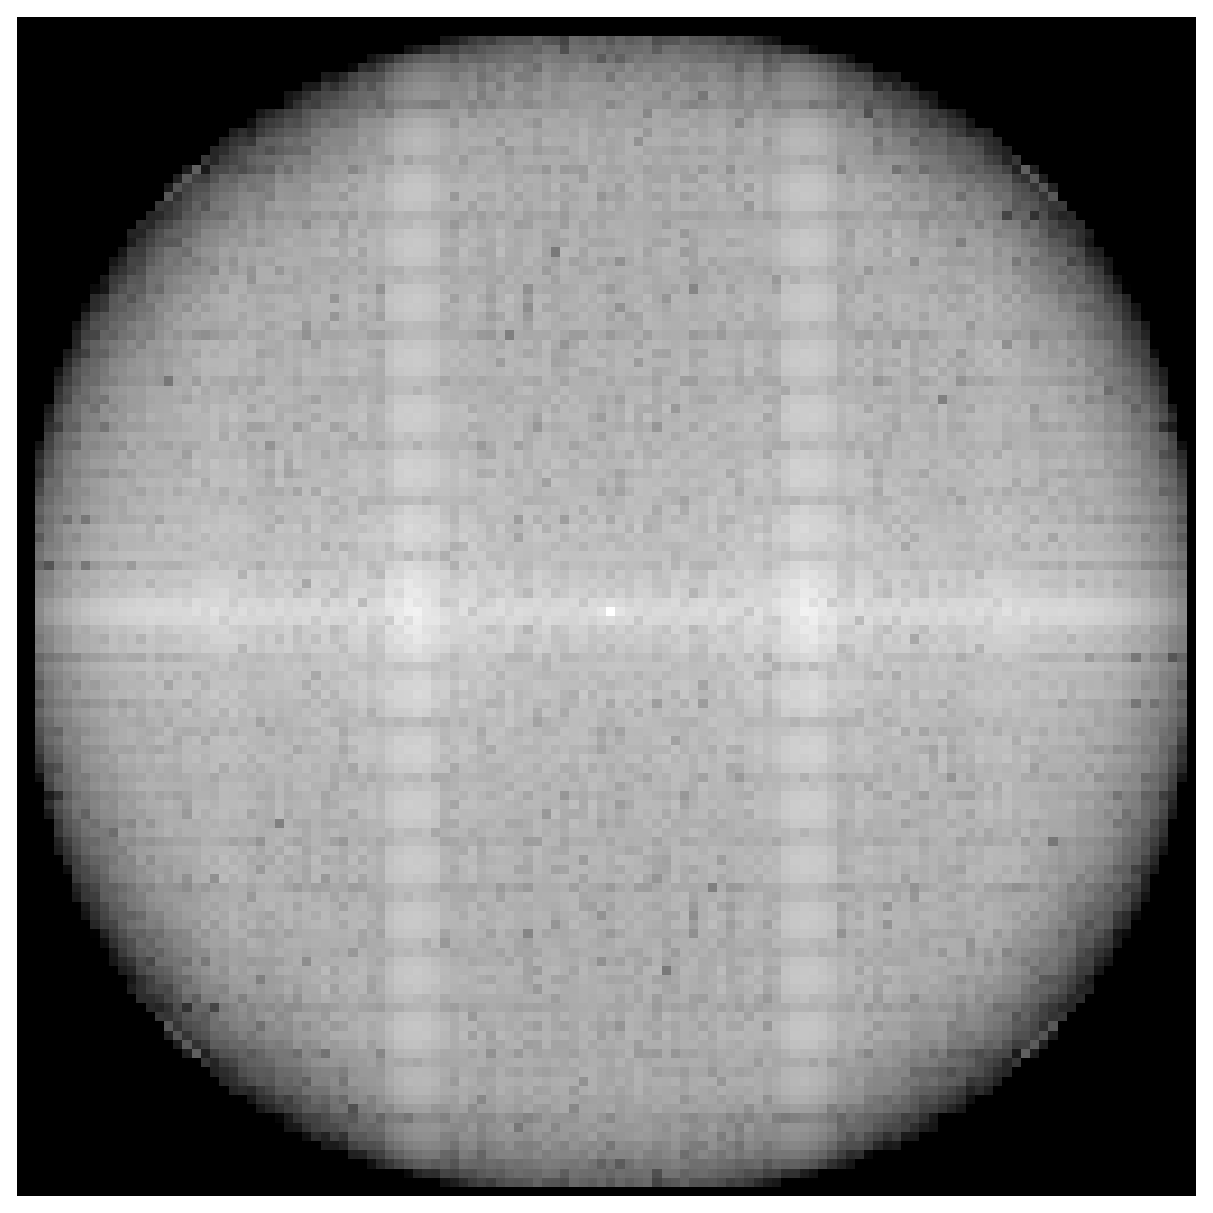
\includegraphics[width=6cm]{../app_hilo/ackin}}
  \subfigure[filtered zero order of uniform image $I_u$ {\sf
    ackiu}]{\label{fig:ackiu}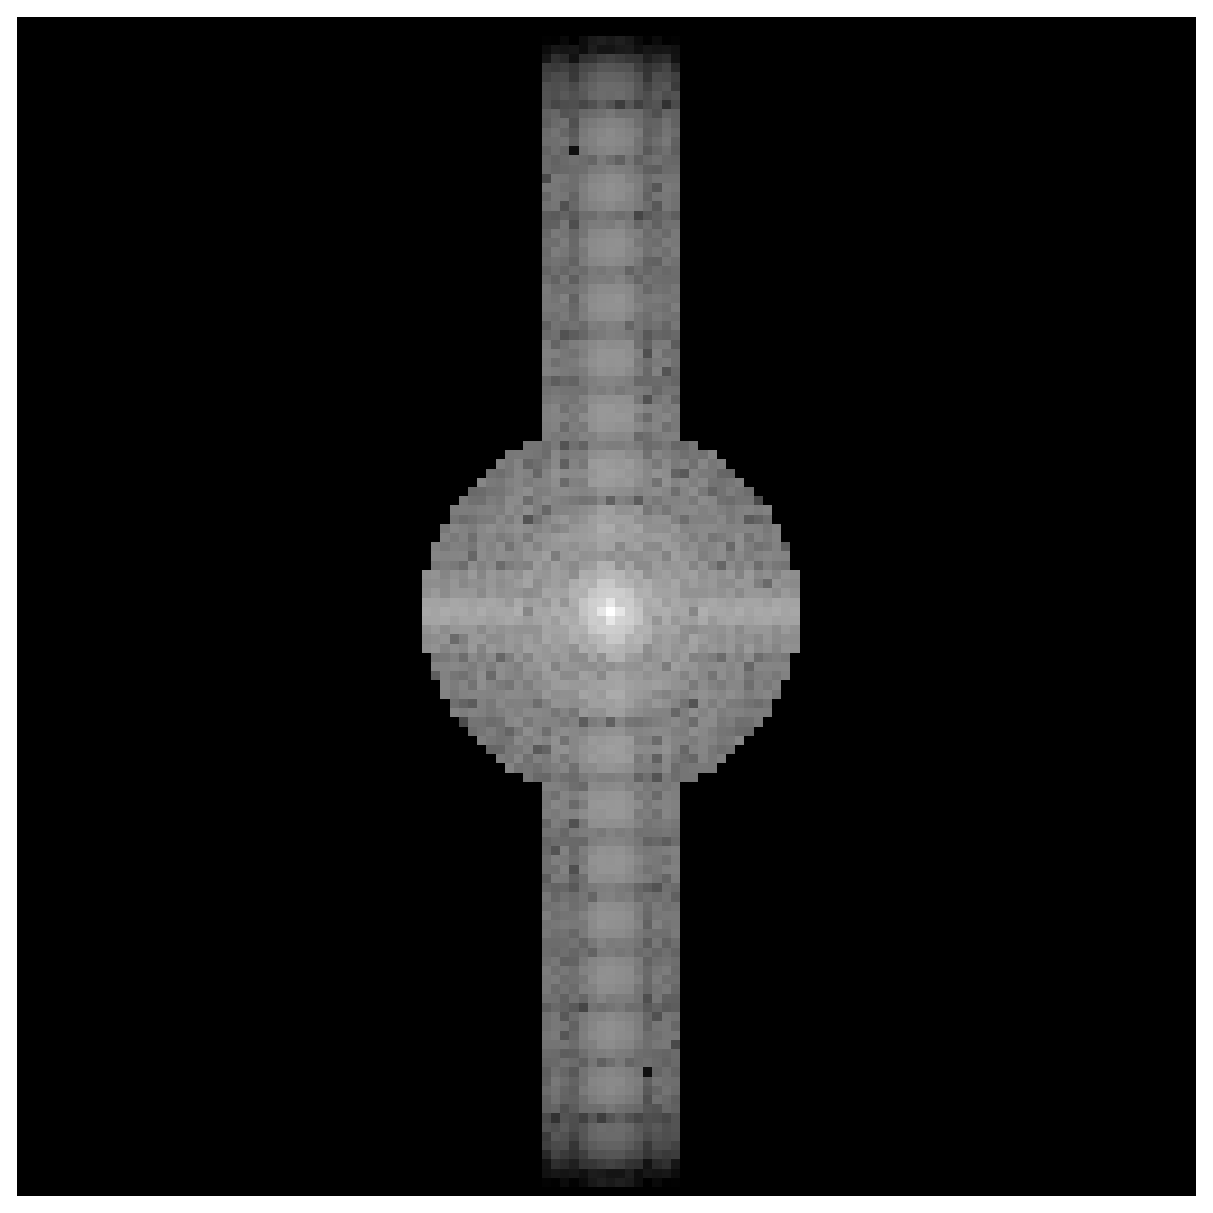
\includegraphics[width=6cm]{../app_hilo/ackiu}}
  \subfigure[Cross correlation
  $cov$.]{\label{fig:cov}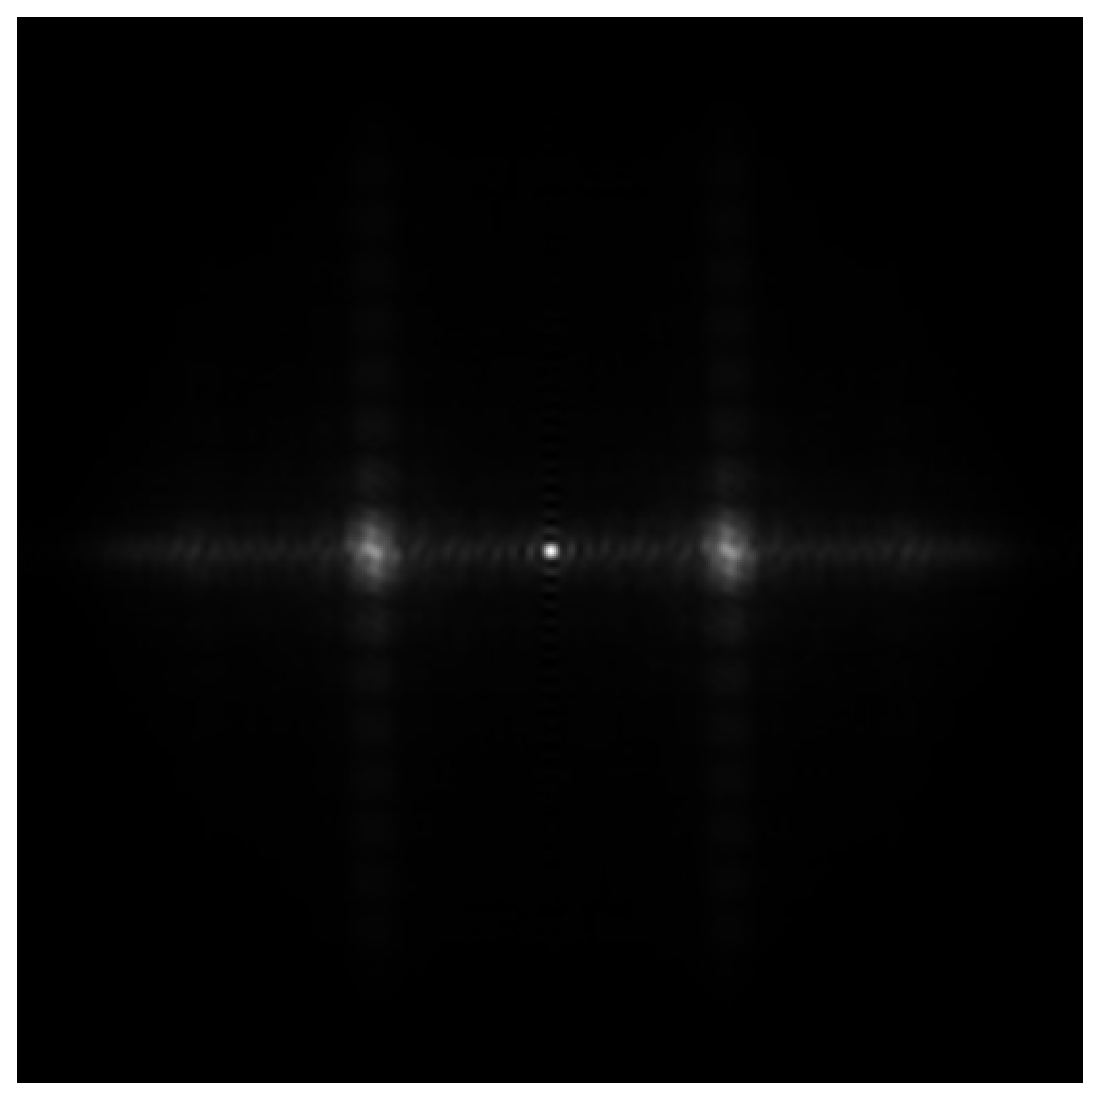
\includegraphics[width=6cm]{../app_hilo/cov}}
  \subfigure[Surface plot of
  $cov$.]{\label{fig:cov3d}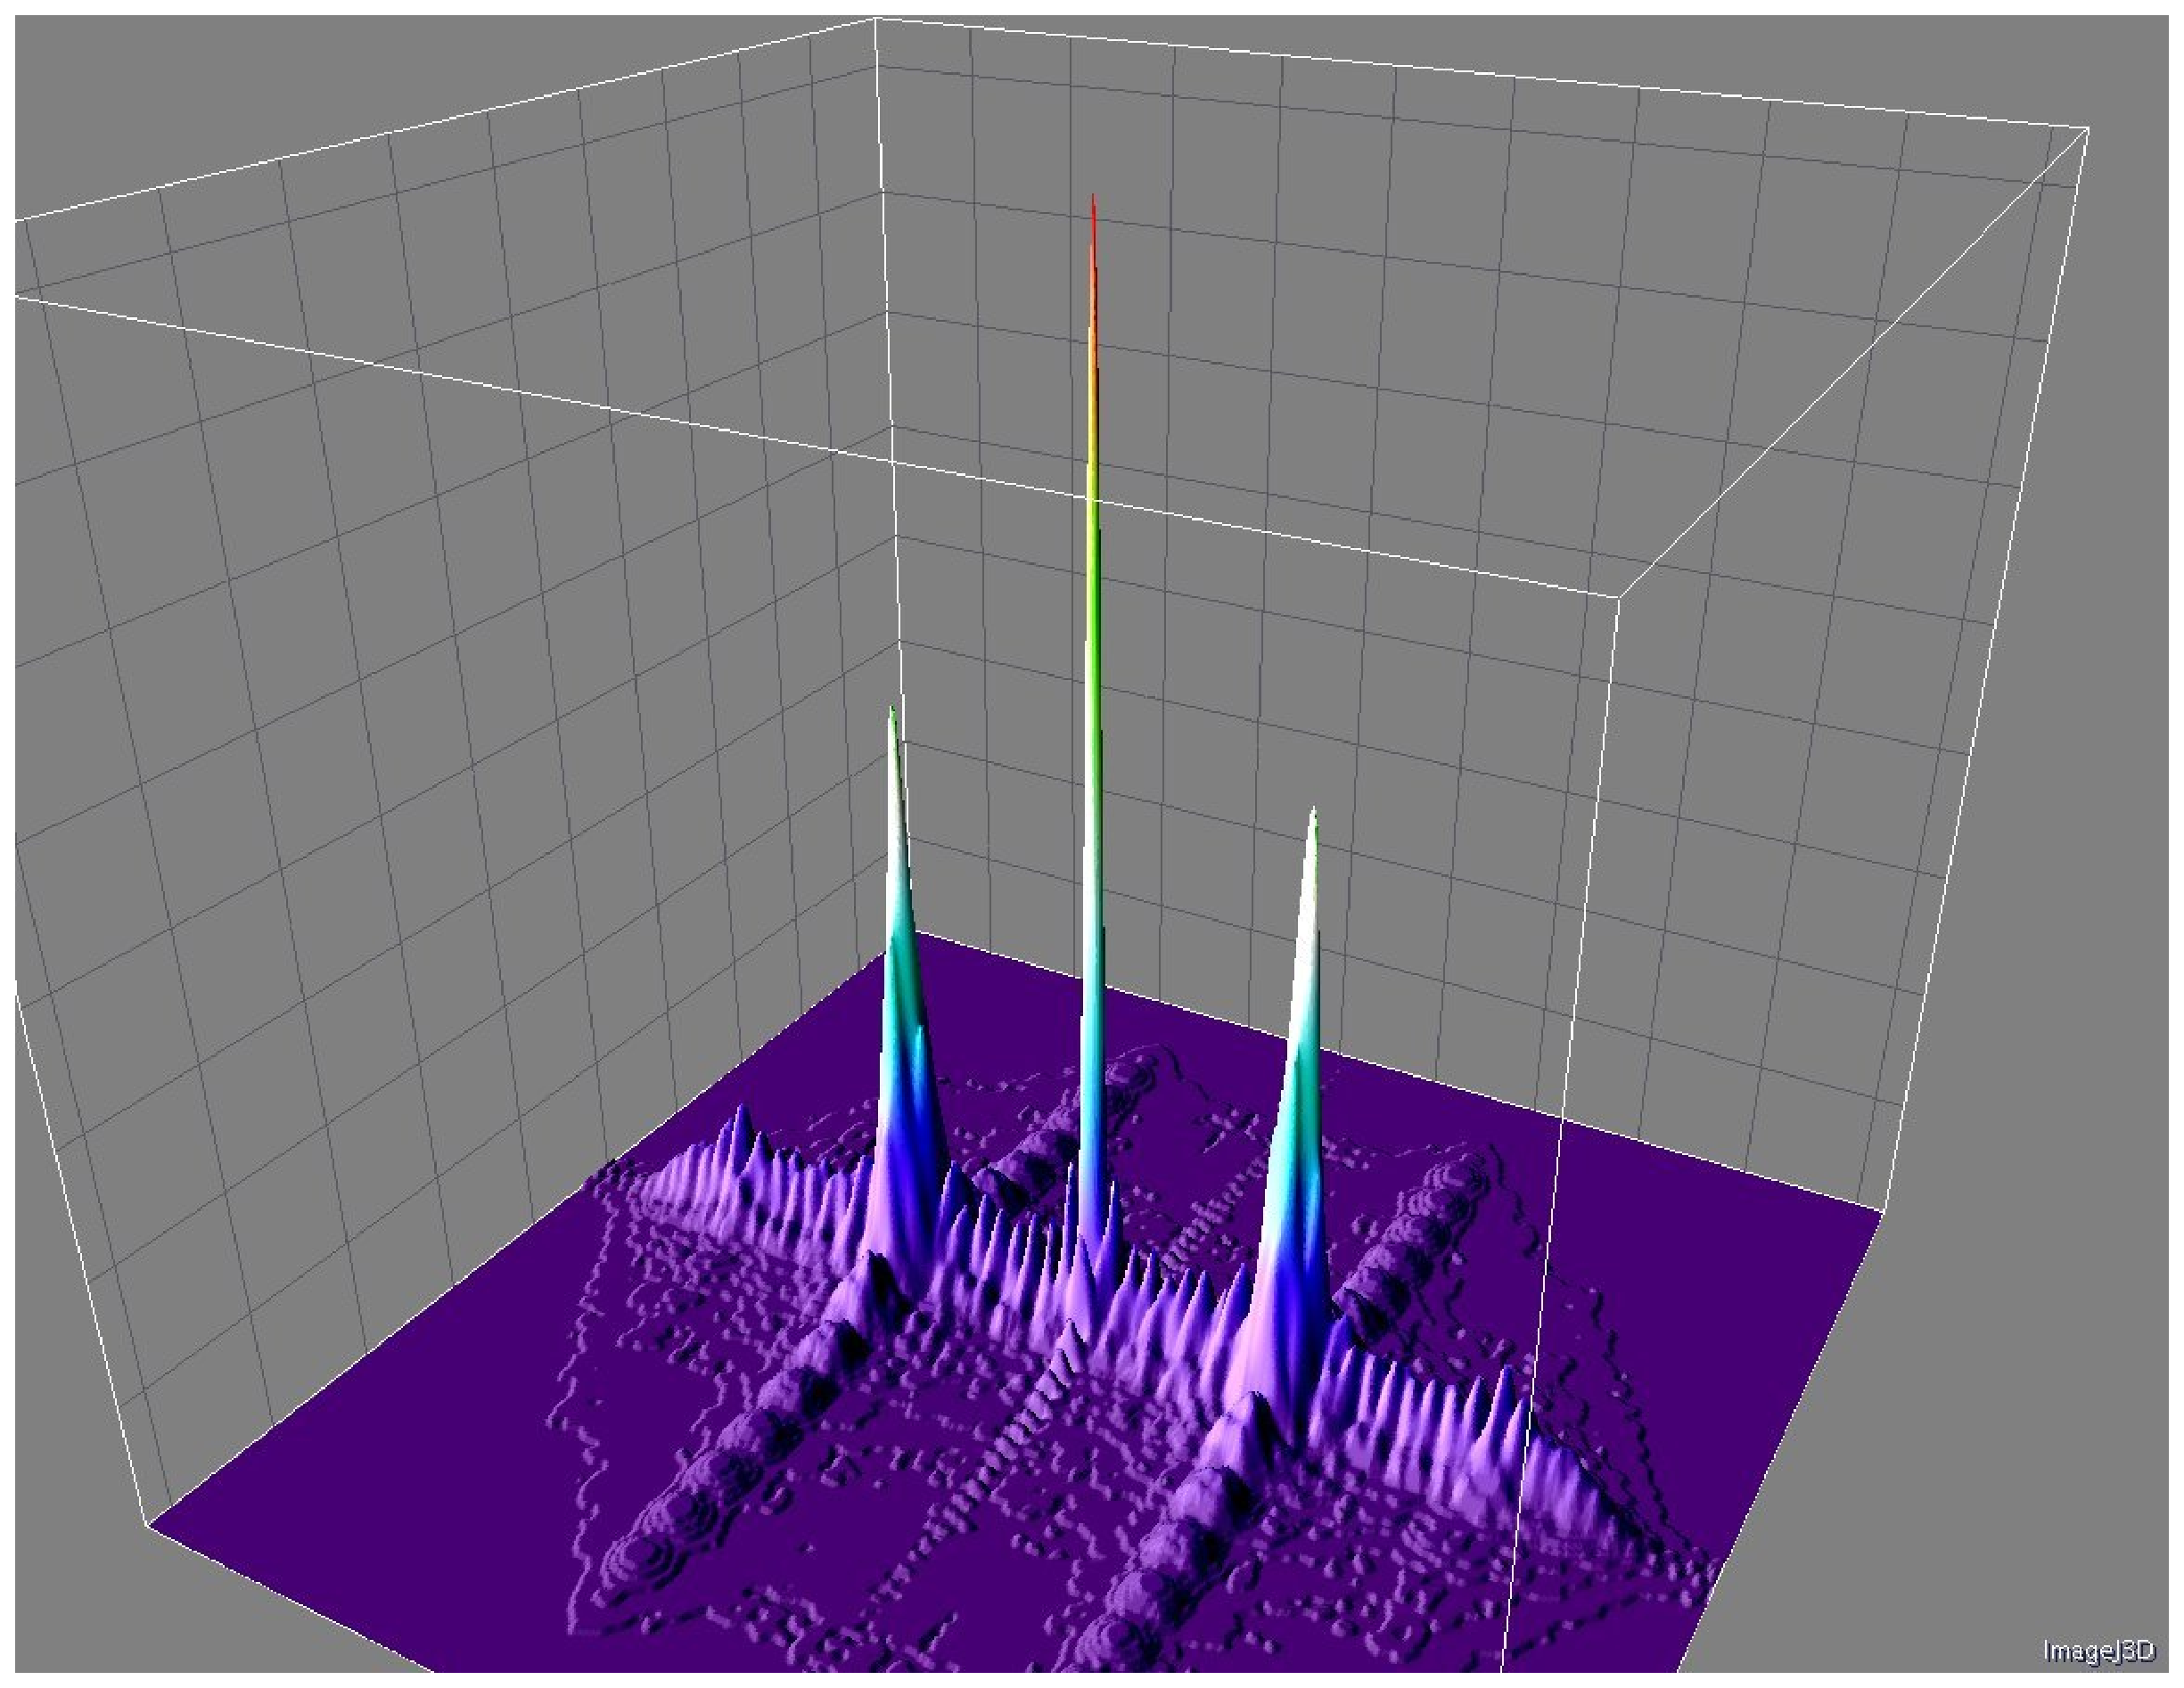
\includegraphics[width=6cm,viewport=100 0
    920 820,clip]{../app_hilo/cov3d}}
  \caption{Intermediate results for the HiLo ``shift'' algorithm.}
  \label{fig:hilo3}
\end{figure}
In order to locate the maximum in the cross-correlation with a
sufficient accuracy the convolution is done on a finer grid by
zero-padding the input images as shown in the following listing:
\begin{lstlisting}
kcov=ft(ackin).*conj(ft(ackiu));
% subsample the correlation by zero padding
kcov_big=newim(512,512)+i-i; % allocate complex array
st=256-64; w=127; en=st+w;
kcov_big(st:en,st:en)=kcov;
cov=abs(ift(kcov_big)); % this contains the cross correlation
\end{lstlisting}
The $512\times512$ image {\sf cov} is shown in \figref{fig:cov} and
\figref{fig:cov3d}. The next listing is the code to locate the centre
of gravity of the nine points on top of the right peak in
\figref{fig:hilo3}~(c,d):
\begin{lstlisting}
%% find maximum on the right of the correlation
startx=75*4;
[m,p]=max(abs(cov(startx:end,:)));
pos=[p(1)+startx,p(2)];
% determine center of mass of the 3x3 region around the maximum
region=abs(cov(pos(1)-1:pos(1)+1,pos(2)-1:pos(2)+1));
region=region-min(region);
cm=[sum(xx(region).*region),sum(yy(region).*region)];
shift=(pos+cm-[256,256])/4 % divide by 4 to undo subsampling
\end{lstlisting}
For the example the displacement {\sf shift} is $(21.25,0)$ relative
to the centre of the $128\times128$ image.
\begin{figure}[htb]
  \centering \subfigure[ $\tilde
  q_s$.]{\label{fig:kqs}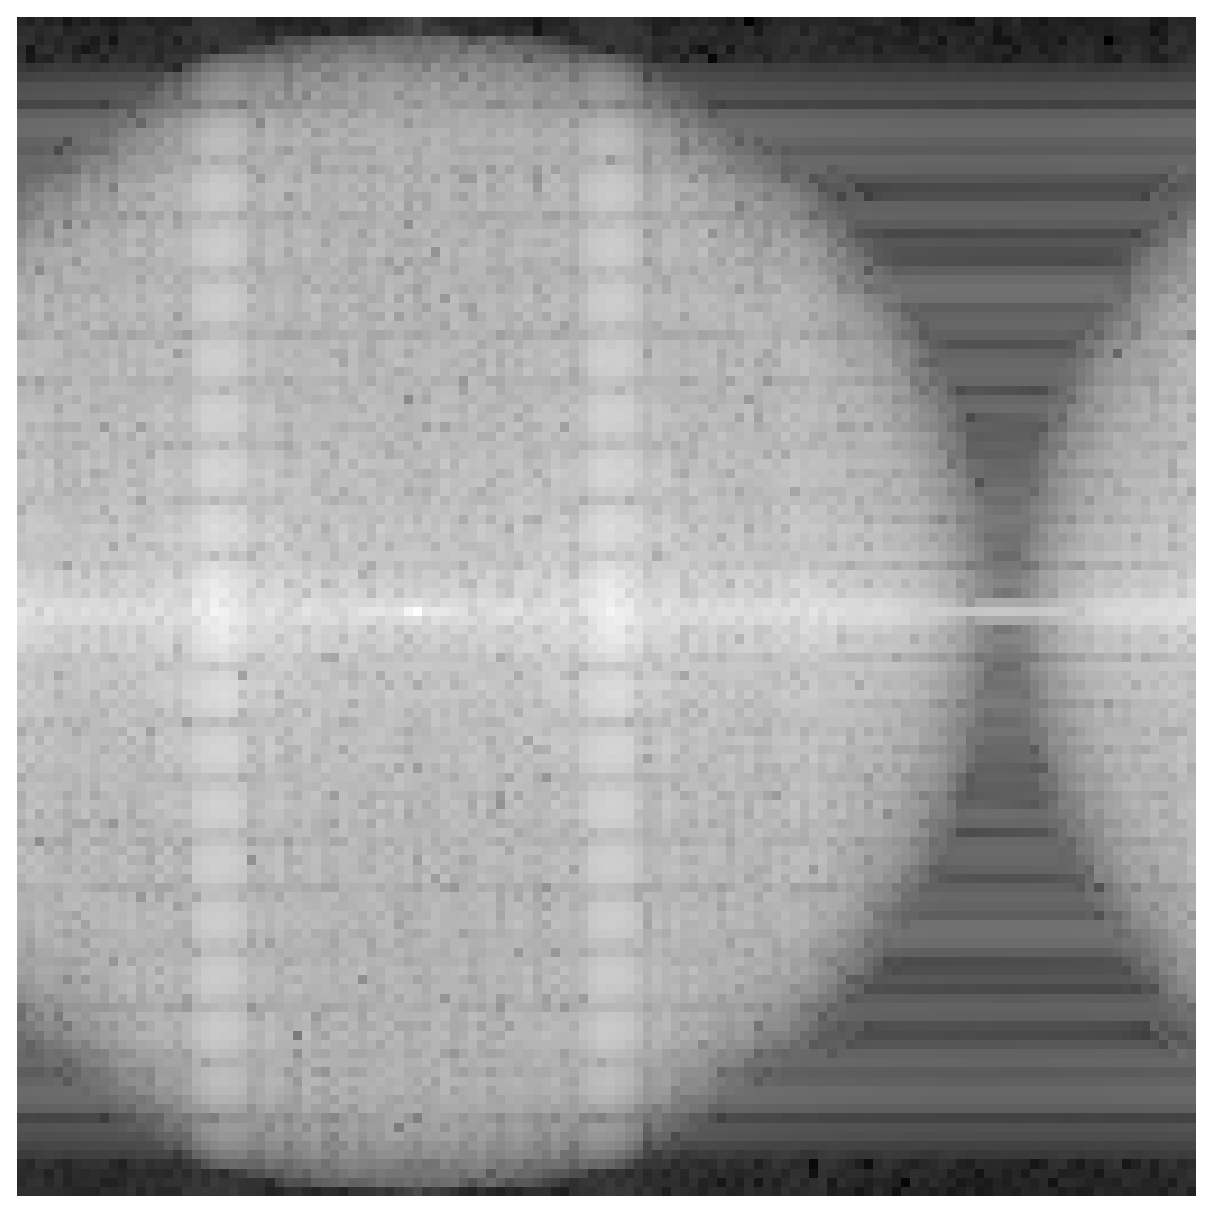
\includegraphics[width=4cm]{../app_hilo/kqs}}
  \subfigure[$\tilde q_s$ with low-pass
  applied.]{\label{fig:kqslp}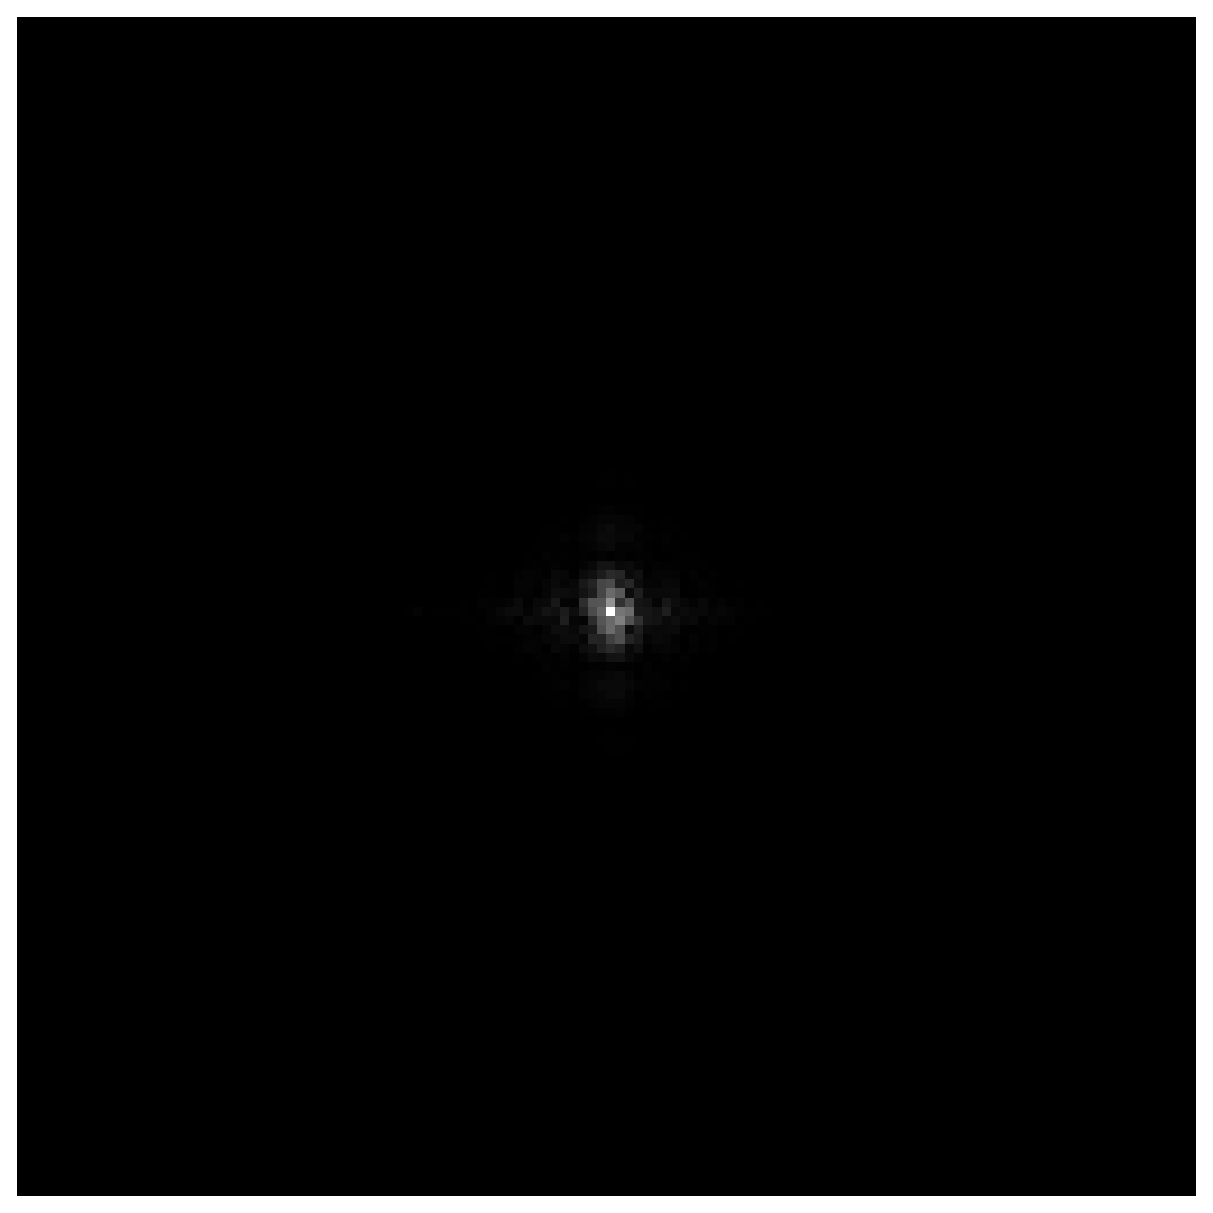
\includegraphics[width=4cm]{../app_hilo/kqslp}}
  \subfigure[$\tilde
  I_\textrm{hp}$]{\label{fig:kihp3}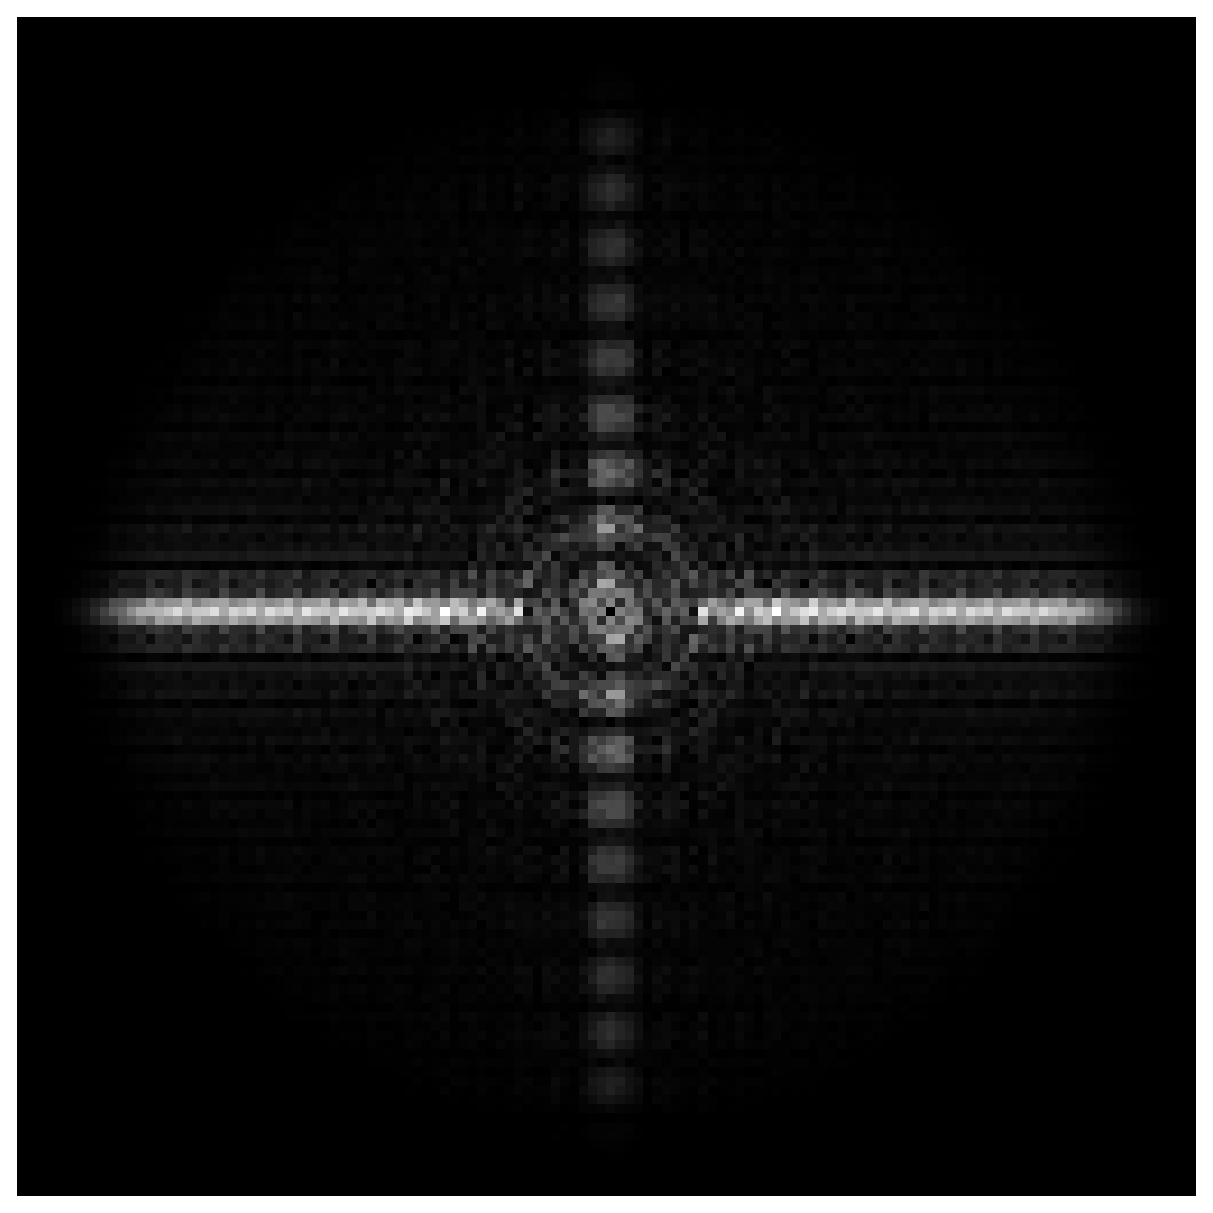
\includegraphics[width=4cm]{../app_hilo/kihp3}}
  \caption{The Fourier transform of the shifted zero-order-suppressed
    non-uniform image $q_s$ with (a) and without (b) low-pass filter
    and the Fourier transform of the corrected high-pass filtered
    uniform image (c). As opposed to all other k-space images (b) and
    (c) are not logarithmic.}
  \label{fig:hilo3_2}
\end{figure}
The following listing shows how the non-uniform image is shifted in
k-space so that the first order becomes DC. The result $\tilde q_s$
is shown in \figref{fig:kqs}.
\begin{lstlisting}
%% multiply by this in object space to shift +1 order into middle
doshift=exp(-i*2*pi*(xx(ckin,'freq').*shift(1)+...
        yy(ckin,'freq').*shift(2)));
kc=0.052;
r=rr(ckin,'freq');
klp=exp(-r.^2/(2*kc^2)); % low pass filter in k-space
q1=ift(ckin-kappa.*ckiu);
kqs=ft(q1.*doshift);
cm=abs(ift(kqs.*klp));
ihp=real(ift(ft(iu).*corr.*(1-klp)));
% integrate over ring with radius kc to find eta
ring=abs(ft(besselj(0,2*pi*kc*n.*r)));
ring2=r-1./n<kc & r+1./n>kc;
cring=ring.*ring2;
nring=cring./sum(abs(cring));
eta=sum(abs(ft(ihp))/abs(ft(cm)).*nring);
% combine highpass and lowpass filtered images
ihilo3=2.*cm+ihp; % don't use eta
\end{lstlisting}
The calculation of $\eta$ gives the value $1.16$. It turns out that
the reconstructed slice (\figref{fig:ihilo3}) looks better with a
value of $\eta=2$. This makes sense as the grating reduces the
illumination power approximately by this factor.
\begin{figure}[htb]
  \centering \subfigure[ {\sf
    cm}]{\label{fig:cm}
\includegraphics[width=4cm]{../app_hilo/cm}}
  \subfigure[$I_\textrm{hp}$]{\label{fig:ihp}\includegraphics[width=4cm]{../app_hilo/ihp3}}
  \subfigure[$I_\textrm{hilo}$]{\label{fig:ihilo3}\includegraphics[width=4cm]{../app_hilo/ihilo3}}
  \caption{Low (a) and high-frequency (b) images in real space and the
    end result (c).}
  \label{fig:hilo3_3}
\end{figure}
\subsubsection{Discussion}
We believe conceptually the subtraction approach is simpler to
understand than the single side-band demodulation method. 

Indeed, long after this section was devised we found \cite{Mertz2010},
where they used a subtraction followed by a rectification
$\abs{I_u-2I_n}$ to partially demodulate the signal.

As a follow up it might be instructive to investigate the performance
of the three different demodulation approaches in the presence of
noise.

\chapter{Sim Angle}
\begin{figure}[!hbt]
  \centering
  \includegraphics[width=12cm]{screen_memi-sim}
  \caption{}
  \label{fig:screen_memi-sim}
\end{figure}

{\small
\begin{verbatim}
n = 128;
nh = n/2;
rad=20;

ka = sinc(rr(n,n,n));
a = ift(ka);
% spherical shell of 1px thickness
% a = xor(rr(n,n,n)<rad,rr(n,n,n)<rad+1);

% select top of the shell, optionally blur
% if bottom half isnt cut away, ke will contain
% rotation symmetric sinc=sin(r)/r
%e = gaussf(a & zz(a)>=0) ; %.2*rad;
e = a * (zz(a)>0);

% show kx-kz display of ewald-sphere
e(:,nh,:)

ke = ift(e);

% xz section of electric field
ke(:,nh,:)

% phase display in xz section of electric field
phase(ke(:,nh,:))

% magnitude in back focal plane of in-focus field
% note that the image isnt uniform due to projection of
% the spherical shell onto a plane
abs(ft(ke(:,:,nh)))

% project sphere shell and threshold to obtain bfp disk
disk = squeeze(max(abs(e),[],3))>.1;

% phase in back focal plane of in-focus field (is zero)
c = ft(squeeze(ke(:,:,nh)));
phase(c) * disk

% transform a defocused slice into back focal plane
defocus=squeeze(ke(:,:,nh-63));
c2 = ft(defocus);
pc2 = phase(c2) * disk

% increase the disk size
zoom = 4;
bigdisk = resample(1.0*disk,[zoom zoom],[0 0],'zoh')
% zero padding to increase sampling of bfp
pc3 = phase(ft(extract(defocus,[zoom*n zoom*n]))) * bigdisk

% resample(real(defocus),[4 4],[0 0],'4-cubic')+j*resample(imag(defocus),[4 4],[0 0],'4-cubic')

% define an lcos pattern
lcx = 0;
lcy = 10;
lw = 32;
lh = 32;
lsx = lcx-lw/2;
lex = lcx+lw/2;
lsy = lcy-lh/2;
ley = lcy+lh/2;
lcos= lsx<=xx(n,n) & xx(n,n)<lex & lsy<=yy(n,n) & yy(n,n)<ley


% define an mma image (with quite low resolution)
mmazoom = 4;
mman = n / mmazoom;
mma = (xx(mman,mman)-3)^2+(yy(mman,mman)-0)^2 < 4^2 ;
intens = newim(n,n,n);
% visit each point in the mma image
for i=0:mman-1
    for j=0:mman-1
        if mma(i,j)
            rphase=newim(n,n);
            rphase(mmazoom*i,mmazoom*j) = 1.0;
            % create corresponding illumination direction on lcos plane
            bfp=ft(lcos .* ift(rphase));
            field=ift(repmat(bfp,[1 1 n]) .* e);
            % accumulate intensity image (incoherent)
            intens = intens+field.*conj(field);
        end
    end
end

intens(:,nh,:)
\end{verbatim}}

%\chapter{MEMI optical system}
\begin{figure}
   \centering
   \def\svgscale{2}
   \input{memi-sketch.eps_tex}
   \caption{Schematic of the lenses in the MEMI system and their focal
     lengths. The focal length $f_\textrm{TL}$ of the tubelens can be
     varied. This allows to scale the second intermediate image
     $r''_\textrm{MMA}$ of the micro mirror array to fit the back
     focal plane of different objectives. Dimensions in mm.}
   \label{fig:memi-sketch}
 \end{figure}
 
\chapter{Experiments with DVI LCoS}

\begin{figure}[!hbt]
  \centering
  \includegraphics[width=14cm]{../dvi/trigger0}
  \caption{}
  \label{fig:trigger0}
\end{figure}


\begin{figure}[!hbt]
  \centering
  \includegraphics[width=12cm]{screen_logic_labels}
  \caption{Snapshot of the trigger signals with a logic analyzer.}
  \label{fig:screen_logic_labels}
\end{figure}

\begin{figure}[!hbt]
  \centering
  \includegraphics[width=14cm]{fast4-no-first_cut}
  \caption{}
  \label{fig:fast4-no-first_cut}
\end{figure}


\begin{figure}[!hbt]
  \centering
  \includegraphics[width=10cm]{dvi-mosaic}
  \caption{}
  \label{fig:dvi-mosaic}
\end{figure}


% talk with nice pictures /mnt/backup/safe-with-time/torben/safed/0321/talk/talk.lisp  amazingly i wrote this presentation in lisp!
% theory /mnt/backup/safe-with-time/torben/safed/0417
% WP6 D6.6 Report on DIC experiments /mnt/backup/safe-with-time/torben/safed/1125
\chapter{Shearing interferometer--based intensity modulation with a
  MEMS mirror device}
\label{sec:app_dic}
\lstdefinelanguage{Maxima}{
keywords={addrow,addcol,zeromatrix,ident,augcoefmatrix,ratsubst,diff,ev,tex,%
with_stdout,nouns,express,depends,load,submatrix,div,grad,curl,%
rootscontract,solve,part,assume,sqrt,integrate,abs,inf,exp},
sensitive=true,
comment=[n][\itshape]{/*}{*/}
}
\lstset{language=Maxima}
\begin{summary}
  Here we describe an alternative approach to turn the micro mirror
  array, which acts as a phase device, into a intensity spatial light
  modulator. The advantage of using this DIC (differential
  interference contrast) method is a higher acceptance angle which
  would lead to a bigger field of view (spatial) in our spatio-angular
  microscope. Eventually the contrast ratios did not surpass those of
  the Fourier method. However, the DIC approach would have been very
  useful if a piston mirror device had been used instead of the
  torsional micro mirrors.
\end{summary}
\section{Introduction}
One of the main partners of the MEMI project is Fraunhofer IPMS
(Dresden, Germany). Before being part of the MEMI project, they
developed a micro mirror array (MMA) with optimized reflectivity in
the ultra violet wavelength range (generation-0). The application of
this device is mainly semiconductor manufacture.

During the MEMI project, they developed a new version of the MMA
(generation-2) that can be used up to near infra red
wavelengths. Initially, Fraunhofer provided generation-0 MMA's to the
project partners.
\begin{figure}[htbp]
  \centering
  \includegraphics[width=7cm]{mma-tilts}
  \includegraphics[width=7cm]{mma-voltages}
  \caption{{\bf left:} Electron micrograph showing generation-2 MMA
    with tilted mirrors. {\bf right:} Schematic of the voltages on one
    mirror (both figures by Fraunhofer IPMS).}
  \label{fig:mma-tilts}
\end{figure}
From the beginning of the project a Fourier filtering--based approach
was planned in order to turn the minute tilts of the micro mirrors
into intensity modulations: An aperture is placed on the zero order of
the Fraunhofer diffraction pattern of the MMA. When mirrors are
tilted, they reflect the light outside of the aperture, where it is
absorbed.

However, the Fourier filtering approach has a drawback: The
illumination angles and the size of the aperture are restricted below
the diffraction angles of the MMA. In our optical system this limits
the area on the LCoS, that can be illuminated and therefore the field
of view in the specimen.

A shearing interferometer--based approach was suggested
instead. There, the images of neighbouring mirrors are overlapped and
can interfere. A system based on Wollaston (or Nomarski or DIC
(differential interference contrast)) prisms would give better angular
acceptance. It promises good contrast and will work for multiple
wavelengths as well. Here we describe experiments that were conducted
on the generation-0 MMA with a set of Nomarski prisms from a Zeiss
differential interference contrast microscope.
\section{Description of the setup}
\begin{figure}[ht]
  \centering
  %\includegraphics[height=9cm]{../app_dic/img/dic_mma}
  \input{dic_mma.eps_tex} % w=87.6mm
  \includegraphics[width=6cm]{../app_dic/img/dsci1331}
  \caption{ Schematic and photograph of the optical setup.  {\bf
      left:} Apertures allow control of the illumination in the planes
    $A''$ and $F''$. The wire grid polarizing beam splitter (PBS) is
    oriented with the aluminium structured side towards the Nomarski
    prism. The Nomarski prism can be rotated around the optical
    axis. {\bf right:} Interference of neighbouring micro mirrors is
    expected for the four angular settings ($\pm 45^\circ$, $\pm
    135^\circ$) of the Nomarski prism.  Here the Nomarski prism is
    oriented in $-45^\circ$ direction.  A white paper card protects
    the wire grid polarizer from dust.  This setup contains two
    additional cleanup polarizers that are not shown in the
    schematic.}
  \label{fig:dic_mma}
\end{figure}
\figref{fig:dic_mma} shows a schematic and a photograph of the setup.
The light source is a liquid light guide--coupled \unit[480]{nm} LED
(CoolLed). It illuminates a square integration rod (\unit[10]{cm}
length) to provide a uniform light distribution in the conjugate
$F'''$ of the field. \nomenclature{DIC}{differential interference contrast}

The optical path for the illumination contains two apertures to
confine the field and to control the illumination angles. We use a
wire grid polarizer (Moxtek, UT, US) as polarizing beam splitter.
Achromatic doublets (objective $f=\unit[200]{mm}$, tube lens
$f=\unit[500]{mm}$) were used as the two imaging lenses.

The position of the focal plane of the Nomarski prisms was estimated
by measuring the distance between the prism and the back focal plane
of the matching micro objectives (the result is generally within
$\unit[2-3]{cm}$). For a flat sample (all MMA mirrors undeflected) we
see a dark band in the interference image. Moving the prism along the
optical axis expands the dark band until it encompasses the full field
of view. We used this to adjust the precise position of the prism.

We selected the prism with the biggest split angle
($\theta=\unit[0.078]{mrad}$, the matching prism for a $63\times/1.4$
oil immersion objective, see section \ref{sec:prism} for the
measurement) in order to keep the distances small and minimize beam
distortion due to air fluctuations. Later we found that the free
aperture of the prism is the limiting factor. For a good DIC effect at
least three orders of the MMA diffraction pattern have to pass through
the prism. Otherwise the prism acts as a Fourier filter. Then the
combined effect of Fourier filtering and (only partial) differential
interference greatly diminishes the contrast of the image.

To reduce the Fourier filtering effect, two identical Nomarski prisms
with \unit[0.078]{mrad} split angle were placed into the setup instead
of one (see \figref{fig:double-prism}). Then we used an objective lens
with shorter focal length. Later we learned that the distance between
the prisms allows to vary the split angle \citep{Schwertner2008}.


\begin{figure}[htb]
  \centering
  \includegraphics[width=5cm]{../app_dic/img/double-prism}
  \caption{Combination of two identical Nomarski prisms to increase
    the split angle between ordinary and extraordinary beam. The prism
    in the experiments are for a $63\times/1.4$ oil immersion
    objective.}
  \label{fig:double-prism}
\end{figure}

\section{Experiments}
\subsection{Procedure to measure the split angle of a Nomarski prism}
\label{sec:prism}
An important task in the beginning was to measure the split angle of
the various Nomarski prisms in our set. The goal was to find a prism
that with a standard lens would give a shear distance equal to the
mirror pitch of the MMA (\unit[16]{$\mu$m}).

The Nomarski prism consists of two quartz wedges. Its function is
based on the birefringence of the crystal. The prism splits a
$45^\circ$ linearly polarized wavefront into two wavefronts with
slightly diverging angles.
\begin{figure}[htb]
  \centering
  \includegraphics[width=8cm]{../app_dic/img/nomarski_split}
  \caption{Setup to measure the split angle $\theta$ of a Nomarski
    prism by interference of the two beams. The polarizers Pol1 and
    Pol2 are crossed and in a $45^\circ$ angle relative to the shift
    axis of the prism.}
  \label{fig:nomarski_split}
\end{figure}
The split is so small that its direct measurement --- illuminating the
prism with a parallel beam and putting the camera into the back focal
plane of a lens with a long focal length --- is difficult.  Instead we
put the prism between crossed polarizers, illuminate it with a
parallel beam and measure a fringe pattern on the camera (see
\figref{fig:nomarski_split} for a schematic of the setup and
\figref{fig:nomarski_split_exp} for the data).

The electrical field $U$ after the second polarizer is:
\begin{align}
  U&=e^{i\vect k_1\vect r}+e^{i\vect k_2\vect r},\\
  \abs{\vect k}&=\frac{2\pi}{\lambda},\\
  \vect k_1&=\abs{\vect k}(0, \hspace{1em}\sin(\theta/2), \cos(\theta/2))^T,\\
  \vect k_2&=\abs{\vect k}(0, -\sin(\theta/2), \cos(\theta/2))^T.
\end{align}
The camera measures the intensity $I$:
\begin{align}
  I=\abs{U}^2=4\cos^2(\abs{\vect k}y\sin(\theta/2)).
\end{align}
Therefore the dark bands have a distance $d$ (for small split angles
$\theta$):
\begin{align}
  d=\frac{\lambda}{2\sin{\theta/2}}\approx \frac{\lambda}{\theta}.
\end{align}
\begin{figure}[htb]
  \centering
  \includegraphics[width=10cm]{../app_dic/img/nomarski_split_exp}
  \caption{Camera image for the prism with the biggest split
    angle. The distance between the two dark fringes is
    $d=\unit[(6.06\pm0.08)]{mm}$. The light source is a laser with
    \unit[473]{nm} wavelength. For the graph, values were integrated
    over the width of the yellow bar to reduce the influence of the
    disturbing fringes.}
  \label{fig:nomarski_split_exp}
\end{figure}
We measured $d=\unit[(6.06\pm0.08)]{mm}$ for the strongest of our
Nomarski prisms.  Other prisms had very small split angles and no two
dark bands could be observed over their clear aperture.

The measured prism has a split angle of $\theta=\unit[0.078]{mrad}$.  For
a lens with a focal distance $f=\unit[200]{mm}$ this corresponds to a
Nomarski split $\Delta x$:
\begin{align}
  \Delta x=2f\tan(\theta/2)\approx f\theta=\unit[(15.6\pm0.2)]{\mu m}.
\end{align}
This is close to the pixel pitch of $\unit[16]{\mu m}$ of the MMA.

\subsection{Imaging the MMA with the DIC method}
\figref{fig:screen5} shows two typical images that can be obtained in
the DIC setup. The schematic in \figref{fig:screen} indicates the
shearing direction and corresponding interference pattern.  For both
images a checkerboard pattern with a periodicity of $16\times16$
elements is displayed on the MMA.

In the right image (\figref{fig:screen} right,
\figref{fig:screen5}~b)) the interference occurs between mirrors that
tilt in different directions (green in the schematic).

Areas on the checkerboard pattern with deflected mirrors appear bright
in the image, regions with flat mirrors are dark. On two edges of the
checkerboard square tilted mirros interfer with flat ones, resulting
in dimmer pixels in the interference image (indicated by purple arrow
in bottom right of \figref{fig:screen5}).

In this configuration it is not possible to produce a perfectly dark
interference next to a deflected mirror.  Therefore, with this shear
direction we cannot display arbitrary gray value images with the
torsion micro mirrors of the MMA.


\begin{figure}[ht]
  \centering
  \includegraphics[width=\linewidth]{../app_dic/img/mma_sketch}
  \caption{Schematic showing how neighbouring mirrors are overlaid by
    the Nomarski prism. $24\times 24$ region of micro mirrors that
    display a checkerboard of $16\times 16$ periodicity. Colour
    indicates neighbouring micro mirrors, that will give rise to
    non-destructive interference in the images on the camera. {\bf
      left:} Prism in $-45^\circ$ orientation. {\bf right:} Prism in
    $+45^\circ$ orientation.}
  \label{fig:screen}
\end{figure}

\begin{figure}[!htbp]
  \centering
  \includegraphics[height=5.9cm]{../app_dic/img/1219/auswert/1checker}
  \includegraphics[height=5.9cm]{../app_dic/img/1219/auswert/2checker}
  \includegraphics[width=7cm]{../app_dic/img/1219/auswert/1checker-section}
  \includegraphics[width=7cm]{../app_dic/img/1219/auswert/2checker-section}
  \includegraphics[width=7cm]{../app_dic/img/1219/auswert/1checker-height}
  \includegraphics[width=7cm]{../app_dic/img/1219/auswert/2checker-height-arrow}
  \caption{{\bf top:} DIC image for a prism setting of $-45^\circ$ (a)
    and $+45^\circ$ (b) (see \figref{fig:screen} for a
    schematic). {\bf middle:} Cross section along the DIC shift
    direction (line marked with 1). {\bf bottom:} Zoom into boxes
    (marked with 2) in the images.  Both DIC images were obtained 
    with two identical sequential DIC prisms (for $63\times/1.4$), a
    \unit[100]{mm} objective lens and a \unit[300]{mm} tube lens.}
  \label{fig:screen5}
\end{figure}

In the other shear direction (\figref{fig:screen} left,
\figref{fig:screen5}~a)) mirrors, that tilt into the same direction,
are brought to interference. Neighbouring mirrors that have the same
deflection result in a black interference image. 

For a bright value in the interference image, both mirrors must be
deflected to a different angle. The closer the two neighbours are in
their deflection angle, the darker their interference image will be.
Therefore it is possible to display arbitrary gray value images in
this configuration.

\subsubsection*{Displaying arbitrary gray value images}

For this, we devised an algorithm that assigns a deflection $d_0$ to
the mirrors on one side of the display and then iterates through the
rows of the goal image that is going to be displayed. For each mirror
$i$ along the row its deflection $d_i(d_{i-1},E_i)$ is calculated in
dependence of the deflection $d_{i-1}$ of the previous mirror and the
goal energy $E_i$ in this pixel.

In the next section we develop a forward model to calculate the energy
$E_i(d_i-d_{i-1})$ of one pixel depending on the deflection difference
between neighbouring mirrors. Using this model we calculate a look-up
table that we invert and use in the algorithm to find the deflections
$d_i$.


\subsection{Forward model for the energy in the interference image}
\begin{figure}[htb]
  \centering
  \includegraphics[width=6cm]{../app_dic/img/dic_prism}
  \caption{ Linearly polarized light is split by the prism into two
    rays with slightly diverging angle. They hit the MMA at two spots,
    which are one shearing distance apart. The light returning through
    the Nomarski prism has different polarization states depending on
    the height difference $h$ of the mirrors at those two beam
    positions.}
  \label{fig:prism}
%http://www.microscopy.fsu.edu/primer/java/polarizedlight/crystalwavefronts/index.html
\end{figure}
First we consider the simplified arrangement of one piston micro
mirror of width $\Lambda$ on a plane mirror (see
\figref{fig:prism}). Later we will use the results of this model and
apply them to the torsion mirrors of the MMA (equation
\ref{eqn:it}). 

Let $k=2\pi/\lambda_0$ with vacuum wavelength $\lambda_0$. We write
the influence of a retarder (the height difference $h$ of the small
piston mirror) on a polarized wave in Jones calculus as
(\cite{Goodman1996} p.~418):
\begin{align}
L_r(\Delta)=\begin{pmatrix}1&0\\ 0&e^{-i\Delta}\end{pmatrix}
\end{align}
with a phase difference $\Delta=2kh$ (the factor 2 due to the
reflection).  The matrix for a polarizer that transmits the component
of the electrical field which is linearly polarized at an angle
$\alpha$ to the x-axis is:
\begin{align}
L_p(\alpha)=\begin{pmatrix}\cos^2\alpha&\sin\alpha\cos\alpha\cr
  \sin\alpha\cos\alpha&\sin^2\alpha\end{pmatrix}.
\end{align}
In our setup (see \figref{fig:prism}) the incoming light has a
$45^\circ$ polarization $\vect U=(1,1)^T/\sqrt{2}$ after the first
reflection on the PBS (not shown in the figure, would be in the
bottom). The light traverses the Nomarski prism which splits it into
two diverging beams of orthogonal polarization. A lens collimates the
beams and then they are reflected by the mirror sample. Here,
depending on the height of the piston mirror, a phase retardation is
imposed on one of the two beams. The reflected light is recombined in
the Nomarski prism and only the component that is polarized at
$\alpha=-45^\circ$ passes through the PBS onto the camera: $\vect
U'=L_p(-45^\circ)L_r(\Delta)$.
\begin{align}
  I'=|\vect U'|^2=(1-\cos\Delta)/2
\end{align}
The camera image is dark for a plane mirror and is maximal for a
piston height $h=\lambda/4$.
%a:-%pi/4;
%r:matrix([1,0],[0,exp(-%i*d)]);
%p:matrix([cos(a)^2,sin(a)*cos(a)],[sin(a)*cos(a),sin(a)^2]);
%expand((p . r . [1,1]) . conjugate(p . r . [1,1]));
For a piston mirror of width $\Lambda$ the energy in the corresponding
pixel on the camera is just the intensity times the area:
\begin{align}
  \Delta(x',y') &=2kh=\textrm{const},\\
  E_\textrm{piston}&=\int_{-\Lambda/2}^{\Lambda/2}\int_{-\Lambda/2}^{\Lambda/2}
  I'(\Delta(x',y'))\,\textrm{d}x'\textrm{d}y'=\frac{\Lambda^2}{2}(1-\cos
  \Delta).
\end{align}
\begin{figure}[ht]
  \centering
  \includegraphics[width=7cm]{../app_dic/img/tilt}
  \caption{ Two mirrors with pitch $\Lambda$. Here they are tilted
    with different deflections $d_1$ and $d_2$ in opposite
    directions.}
  \label{fig:tilt}
\end{figure}
As the mirrors of the MMA tilt (and don't move like pistons) it is
necessary solve the integral of the intensity along the DIC shift
direction $x'$ to get the energy in one pixel depending on the tilt of
the two neighbouring mirrors (this calculation is done for small
mirror tilts, see \figref{fig:tilt}):
% Delta = 2kh; 
% integrate((1-cos(2kh))/2,x,-l/2,l/2);
% h(l) = d, h(-l) = d, h(0) = 0
% h(x) = abs(d*x/l) 
% 2*integrate((1-cos(2*k*d*x/l))/2,x,0,l/2);
\begin{align}
\label{eqn:it}
\Delta(x',y') &= 2kh(x') = 2k\frac{\abs{x'} \delta}{\Lambda},\\
E_\textrm{torsion}&=\int_{-\Lambda/2}^{\Lambda/2}\int_{-\Lambda/2}^{\Lambda/2}
I'(\Delta(x',y'))\,
\textrm{d}x'\textrm{d}y'=\frac{\Lambda^2}{2}\left(1-\frac{\sin(k
    \delta)}{k \delta}\right).
\end{align}
Here $\delta=d_1-d_2$ is the difference between the deflections $d_1$
and $d_2$ of the two mirrors and $\Lambda$ is the mirror pitch. If the
deflections $d_1$ and $d_2$ have opposite signs, the mirrors tilt in
opposite directions. Note that the integral sums incoherently across
the mirror because in our experiment we use a LED light source.

Equation \ref{eqn:it} is the forward model. It describes the energy
$E_\textrm{torsion}(d_1-d_2)$ in one pixel of the interference image
depending on the deflections of two neighbouring
mirrors. \figref{fig:erika-detail}~a) shows a gray value image that
should be displayed in the interference image. The corresponding
pattern on the micro mirror array is depicted in b). The image c)
contains the interference image as acquired by the camera.

\begin{figure}[!htbp]
  \centering
  \includegraphics[width=.8\linewidth]{../app_dic/img/1219/auswert/erika-detail}
  \caption{{\bf (a)} Closeup of the input image. {\bf (b)} The
    precomputed (with the look up table algorithm) image that is
    displayed on the MMA. The DIC shift will occur from the left top
    towards the right bottom. Note that regions that are white in the
    input image have a grating structure with high contrast. {\bf (c)}
    The resulting interference image on the camera. For this image we
    used two identical Nomarski prisms in series (for $63\times/1.4$), a
    \unit[100]{mm} objective lens and a \unit[300]{mm} tube lens.}
  \label{fig:erika-detail}
\end{figure}

% sin(a) = m*lambda/Lambda
% asin(473.0/16000) = .0295 rad = 1.694 degree
% tan(a) = r/f -> r = 200 mm * tan(0.0295) = 5.9 mm;
% tan(asin(473/16000))*200

\subsection{Effects of limited prism aperture on DIC image of
  torsional mirrors}
\label{sec:size}
The light coming back from the MMA produces a Fraunhofer diffraction
pattern in the plane $A'$ approximately at the Nomarski prism (see
\figref{fig:dic_mma}). The clear aperture of our prisms is about
\unit[10]{mm}. The first orders due to the \unit[16]{$\mu$m} pixel
pitch of the MMA are at \unit[$\pm5.9$]{mm} with an objective lens of
\unit[200]{mm} focal length.

In order to investigate the influence of the blocking the
$\pm1^\textrm{st}$ orders, we added a circular aperture into plane
$A'$ (\figref{fig:dic_mma}) and captured interference images for
various diameters of this aperture (see \figref{fig:erikas}).  The
schematic above the images depicts the size of the circular aperture
in relation to the diffraction pattern of the MMA.

With decreasing aperture diameter streaks in the images (red arrows)
become more pronounced. These artefacts originate in regions on the
pattern, that is shown on the MMA that differ from their surrounding
rows. 

\begin{figure}[!htb]
  \centering
  \includegraphics[width=.8\linewidth]{../app_dic/img/streaks2}
  \caption{When the $\pm1^\textrm{st}$ orders do not pass through the
    Nomarski prism, unwanted artefacts arise.  These images were
    obtained with one Nomarski prism (for $63\times/1.4$ micro
    objective) a \unit[200]{mm} objective lens and a \unit[500]{mm}
    tube lens.}
  \label{fig:erikas}
\end{figure}
\begin{figure}[!hbtp]
   \centering
   \includegraphics[width=7cm]{../app_dic/img/1219/auswert/erika-streak-overview}
   \caption{Pattern that is displayed on the MMA for the images in
     \figref{fig:erika-detail}~c) and \figref{fig:erikas}. The shear
     direction is from top left to bottom right.}
   \label{fig:erika-streak-overview}
 \end{figure}
\section{Discussion}
We showed that a differential interference approach can be used to
convert the micro mirror array into an intensity spatial light
modulator. It is necessary that the $\pm1^\textrm{st}$ diffraction
orders contribute to the interference image. The best results were
obtained by two Nomarski prisms (each \unit[0.078]{mrad} split angle
and \unit[10]{mm} clear aperture) in series and an objective lens with
\unit[100]{mm} focal length. In this configuration the
$\pm1^\textrm{st}$ diffraction orders are $\unit[\pm2.9]{mm}$
off-axis. This leaves ca.\ $\unit[2.1]{mm}$ for illumination angles
and therefore not much more than the angular acceptence of a Fourier
filtering based approach, which could accommodate a radius of
$\unit[1.4]{mm}$.

The differential interference approach is a promising candidate to
convert piston mirror devices into intensity modulators.

% calibration of heo /mnt/backup/safe-with-time/torben/safed/y2009/0512
% measurement double plane /mnt/backup/safe-with-time/torben/safed/0525
% talk /mnt/backup/safe-with-time/torben/safed/0321/talk
\chapter{Holographic approach to spatio-angular illumination}
\begin{summary}
  Here we present an alternative system for spatio-angular control. It
  is based on a single phase-only LCoS. This simplifies electronic
  synchronization.
\end{summary}

\section{Introduction}
In this part we describe a very different approach that simplifies the
setup considerably.

\begin{figure}[!hbt]
  \centering
  \input{holo-setup3.eps_tex}
  \includegraphics[height=1cm]{hologram-disk}
  \caption{Schematic of the holographic spatio-angular microscope. A
    phase only LCoS in the intermediate image plane displays a grating
    and steers the first order into the back focal plane of the
    objective. Period and orientation define the angle of the
    illumination in the sample. Shape and contrast of the grating
    define the illuminated area and intensity of the illumination.}
  \label{fig:holo-setup3}
\end{figure}

\figref{fig:holo-setup3} shows a schematic of the setup. The main
component is a phase-only spatial light modulator in the intermediate
image plane. When nothing is displayed on the spatial light modulator,
it will reflect the Gaussian laser beam into a beam dump, so that
the light cannot enter the tubelens.

\section{Description of the holographic method}
The spatial light modulator is then programmed to display a phase
grating.  The direction and periodicity of a grating can be chosen
such that the first order is steered into any position on the back
focal plane. In the sketch the grating directs the first order into
the periphery of the back focal plane. Therefore the specimen will be
illuminated by light under a steep angle (not visible in
\figref{fig:holo-setup3} due to exaggerated focal length of
objective).

Decreasing the size of the grating will decrease the size of the
illuminated area in the object. Note that a grating of very small size
gives rise to a wide first order in the back focal plane, limiting the
possible angular control.
\subsection{Description of the experimental setup}
We use a HEO 1080 P High-Resolution LCOS Phase Only Spatial Light
Modulator (Holoeye, Berlin, Germany) to control the phase in the
intermediate plane. The light source is a \unit[473]{nm} DPSS diode
laser. It is coupled into a polarization maintaining fibre and
collimated by a \unit[150]{mm} lens with \unit[50]{mm} diameter.

The tube lens has \unit[300]{mm} diameter and the objective is a
$63\times/1.4$ with oil immersion.  For aligning the optical system a
sequence of device filling gratings was displayed at 60Hz. The
parameters of the grating were chosen such that the first order
describes a circle in the back focal plane.

\subsection{Description of the sample}
To show that the illumination angle of the light was indeed adjustable
a test sample was constructed. A slide and a cover slip were coated
with a thin fluorescent plane (see \figref{fig:holo-setup3}). The air
gap between the two fluorescent planes was approximately five
micrometres thick.

Imaging the fluorophore plane on the slide resulted in a haze of
background fluorescence stemming from the cover slip (see
\figref{fig:holo-meas}). Changing the illumination angle resulted in a
rotation of this haze as one would expect.
\begin{figure}
  \centering
  \includegraphics[width=12cm]{haze}
  \caption{Widefield images of a sample of two parallel fluorescent
    planes with varying azimuth angle of the illumination (numbers in
    in degree). One of the fluorescent planes is in focus, the other
    is imaged as an unsharp haze.}
  \label{fig:holo-meas}
\end{figure}

\section{ Characterization of the phase-only spatial light modulator}
\begin{summary}
  Here we measure the correspondence between displayed gray values and
  resulting phase difference on the Holoeye HEO 1080P spatial light
  modulator.
\end{summary}
We use a similar setup as given in the manual \citep{Holoeye2006}.
\begin{figure}[!hbt]
  \centering
  \includegraphics[width=16cm]{sketch}
  \caption{Setup for calibrating the transfer function of the phase
    SLM. We will establish, which gray values correspond to what phase
    delay. The light from a polarization maintaining single mode fibre
    is circularly polarized by a $\lambda/4-$plate and a polarizer is
    then used to select the optimum polarization direction. The
    Fraunhofer diffraction pattern of light, which has been reflected
    from the device, is captured with a fast camera. (The display's
    cable would come out at the top, perpendicular to the paper
    plane.)}
  \label{fig:holo-calib}
\end{figure}
The SLM is illuminated with a parallel linearly polarized wave
front. The plane of vibration of the electric field is in the paper
plane.

The SLM displays two vertical bars. The left bar shows black (0) and
the upper bar displays a gray value that is varied for the
measurement.  The beam has a circular shape and a (sufficiently)
constant intensity distribution. The beam is centred on the line
between the two bars of different phase. 
\subsection{Numerical simulation}
The minima of the diffraction pattern in the Fourier plane (on the
camera) move proportional to the phase difference between the two
parts of the display (see \figref{fig:holo-theory}).
\begin{figure}[!hbt]
  \centering
  \includegraphics[width=12cm]{theory}
  \caption{Theoretical simulation of the Fraunhofer diffraction
    pattern for varying phase difference between the two sides of the
    display.}
  \label{fig:holo-theory}
\end{figure}
For the simulation we calculated the Fourier transform of a phase
image with a geometry as shown in the top left image in
\figref{fig:holo-theory}.  The three images on the right show the
Fraunhofer diffraction patterns of this (reflective) phase image for
three different values of the phase difference between the half
circles. The position of the minimum changes proportionally to the
phase difference. Therefore we can measure the position of the extrema
to determine the relationship between gray value and phase difference
(the transfer function of the device).

\subsection{Measurement}
The result of this measurement is shown in the top of
\figref{fig:holo-transfer}
(horizontal section through centre of
the Fourier pattern against gray value)
\begin{figure}[!hbt]
  \centering
  \includegraphics[width=16cm]{measure}
  \caption{{\bf top:} horizontal sections through the Fraunhofer
    diffraction pattern on the camera are plotted as columns. The
    displayed gray value is plotted as the x-axis. {\bf bottom:} Time
    variation of the phase, when a constant value of 170 is shown. The
    phase fluctuates considerably.}
  \label{fig:holo-transfer}
\end{figure}
The measurement shows that a phase difference of $2\pi$ can be induced
for a sufficiently high gray value. However we observe significant
noise for the phase measurements.  There are jumps in the data that
amount to several 10 gray values. 

To analyze this effect further a fast camera (mvBlueFox 102G, 2400 Hz,
$200\times4$ region of interest, $\unit[ 6]{\mu m}$ pixel size) was
used to image the Fourier pattern with a high time resolution.  The
bottom image in \figref{fig:holo-transfer} displays 1000 horizontal
line sections over the centre of the Fourier plane. In the beginning,
both half circles were displaying a gray value of zero. Then the right
half circle was suddenly set to 170. The transient occurs quite fast
but then there is a waveform with 5 peaks that repeats with 50 Hz (the
refresh rate of the display).

The measurement suggests that the phase difference of the Holoeye SLM
is varying significantly over time. In order to improve the
performance for displaying computer generated holograms we could
trigger the laser only for a short time before a new frame will be
displayed.

From other experiments we know that there is also cross talk between
the pixels, i.e. if a fine grating is displayed, the displayed phase
contrast is lower than for a coarser grating.
\section{Conclusion}
With our prototype system we showed that it is possible to use the
phase-only SLM to achieve angular and spatial control of the
illumination. Further work would be necessary to optimize the grating
fine structure in order to direct more light is directed towards the
first order (blazing).

Compared to the MEMI system a lot less synchronization between devices
is necessary. However, this technique is only possible with coherent
illumination. Furthermore there is no inherent advantage in the
holographic method as light from dark areas is sent into a beam stop
and is lost as in the MEMI system.

It might be possible to build a system using a kinoform element (two
phase holograms in different positions). This would allow to redirect
light from dark areas into bright areas leading to a much more
efficient system. A different display device with less cross talk
and fluctuations would be advisable for this.


\renewcommand{\(}{\left(}
\renewcommand{\)}{\right)}
\chapter{Equidistant spiral sampling}
\begin{summary}
  In our system the MMA is imaged into the circular back focal plane
  of the microscope objective. Here we propose a method of storing
  images of circular apertures in its linear frame buffer.
\end{summary}
\section{Archimedes Spiral}
An Archimedes spiral in polar coordinates $(r,\theta)$ is defined like
this:
\begin{align} \label{eqn:def}
  r(\theta)=a\,\theta.
\end{align}
The step height $h$ of the spiral is constant and given by
\begin{align}
  h=\abs{r(\theta)-r(\theta+2\pi)}=r(2\pi)=2\pi a.
\end{align}
We would like to distribute circular windows at equidistant points
along the spiral \citep{Ahn1983}.
\section{Equidistance sampling}
We want to start sampling in the center at $r(0)=0$ and sample the arc
length of the spiral with equidistant points. The arc length of an
archimedes spiral is \citep{Weisstein}:
\begin{align} \label{eqn:arclength}
  s(\theta)=\frac{a}{2}\(p\,\theta + \log(p\,\theta)\)\quad\textrm{with}\quad
  p=\sqrt{1+\theta^2}.
\end{align}
The arc length $\Delta s$ between successive points along the spiral
should be equal to the step height $h$. Starting from the central
point $\theta_0=0$ the arc length where to sample the $i-$th point can
be obtained by inverting equation \eqref{eqn:arclength}:
\begin{align}
  \theta_i=\theta(i\,\Delta s).
\end{align}
This inversion can be done efficiently with Newton iteration:
\begin{align}
  x_0&=1,\\
  x_{n+1}&=x_n-\frac{f(x)}{f'(x)}.
\end{align}
Here we introduce the function $f(\theta)$ that vanishes at a given arc
length $s$ and its derivative $f'(\theta)$:
\begin{align}
  \label{eqn:f}
  f(\theta)&=\frac{a}{2}\(p\,\theta+\log(p\,\theta)\)-s,\\
  f'(\theta)&=\frac{\partial f(\theta)}{\partial \theta}=
  \frac{a}{2}\frac{(1+2\theta^2)(1+p\theta)}{p^2 \theta}.
\end{align}
\section{Filling the back focal plane}
We want to find the coordinates of equaly distributed sampling points
along the arc length inside of a circle with radius R. We put the
first sampling point $\theta_0=0$ in the center and the last point
$\theta_n$ on the periphery of the circle. By definition
\eqref{eqn:def} of the spiral we know
\begin{align}
  \theta_n=R/a.
\end{align}
Now we obtain the arc length $s(\theta_n)$ of the spiral contained
inside the circle via \eqref{eqn:arclength}. Dividing by the number of
sub-intervals gives the apropriate sampling step $\Delta s =
s(\theta_n)/(n-1)$.

Note that we are only interested in solutions with $\Delta s=h$. We
want the sampling step to be equal to the step height $h=2\pi a$ of
the spiral. We therefore need to find the zero of the function:
\begin{align} \label{eqn:g}
  g(a)&=\frac{s(\theta_n)}{n-1}-2\pi a\\
  &=\frac{a}{2}\frac{p\theta_n+\log p\theta_n}{n-1}-2\pi a\\
  &=\frac{a}{2}\frac{\sqrt{1+\frac{R^2}{a^2}}\frac{R}{a}+
    \log\(\sqrt{1+\frac{R^2}{a^2}}\frac{R}{a}\)}{n-1}-2\pi a.
\end{align}
We know $a\not =0$ therefor we can transform the function to simplify
its derivative:
\begin{align} \label{eqn:g1}
  g_1(a)&=\underbrace{\sqrt{1+\frac{R^2}{a^2}}}_{p_1}\frac{R}{a} 
  +\log\(\sqrt{1+\frac{R^2}{a^2}}\frac{R}{a}\)-4\pi (n-1),\\
  g_1'(a)&=-\frac{R^3}{p_1}\frac{1}{a^4}-\frac{R^2}{p_1^2}\frac{1}{a^3}-R
    p_1\frac{1}{a^2}-\frac{1}{a}.
\end{align}
Newton's method can be used to find the zero $a_0$ of $g(a)$. Then
$\Delta s$ can be obtained and the circle drawn.

% for i in *.pgm ; do potrace $i ;done
\begin{figure}[h]
  \begin{center}
    \includegraphics[width=.3\columnwidth]{../app_spiral/o0030}
    \includegraphics[width=.3\columnwidth]{../app_spiral/o0100}
    \includegraphics[width=.3\columnwidth]{../app_spiral/o0200}
    \includegraphics[width=.3\columnwidth]{../app_spiral/o0300}
    \includegraphics[width=.3\columnwidth]{../app_spiral/o0400}
    \includegraphics[width=.3\columnwidth]{../app_spiral/o1024}
  \end{center}
  \caption{Equidistant sampling of a circle of the same radius
    $R=128$ with different number of points (from top left to bottom
    right: 30, 100, 200, 300, 400, 1024).}
\end{figure}

\section{Improvement for sampling with disks}
It is useful to modify the filling formula \eqref{eqn:g} such, that
disks with radius $r_s=\alpha\Delta s/2$ on the sample points don't
overlap the periphery of the big circle. Again we have $\theta_n=R/a$ but $R$ is smaller than the back focal plane radius $R_B$:
\begin{align}
  R=R_B-r_s.
\end{align}
Thus we can define the equivalent to \eqref{eqn:g1}:
\begin{align}
  \begin{split}
  g_2(a)&=\overbrace{\sqrt{1+\frac{(R_B-\pi\alpha a)^2}{a^2}}}^{p_2}
  \frac{R_B-\pi\alpha a}{a}+
  \log\(\sqrt{1+\frac{(R_B-\pi\alpha a)^2}{a^2}}\frac{R_B-\pi\alpha a}{a}\)\\ 
  &-4\pi (n-1),\end{split}\\
  g_2'(a)&=
  -\frac{R^3}{p_2}\frac{1}{a^4}
  -\(\frac{\pi\alpha R^2}{p_2}+\frac{R^2}{p_2^2}\)\frac{1}{a^3}
  -\(R p_2+\frac{\pi\alpha R}{p_2^2}\)\frac{1}{a^2}-\(\pi\alpha p_2+1\)\frac{1}{a}+\frac{\pi\alpha}{R}.
\end{align}


\begin{figure}[h]
  \begin{center}
    \includegraphics[width=.3\columnwidth]{../app_spiral/q0030}
    \includegraphics[width=.3\columnwidth]{../app_spiral/q0100}
    \includegraphics[width=.3\columnwidth]{../app_spiral/q0200}
    \includegraphics[width=.3\columnwidth]{../app_spiral/q0300}
    \includegraphics[width=.3\columnwidth]{../app_spiral/q0400}
    \includegraphics[width=.3\columnwidth]{../app_spiral/q1024}
  \end{center}
  \caption{A back focal plane of radius 100 is filled with equidistant
    spiral sampling, ensuring that the outermost disk is contained
    inside. The number of disks are (from top left to bottom right):
    30, 100, 200, 300, 400, 1024.}
\end{figure}

\section{Discussion}
It is possible to distribute sample points along a spiral over the
back focal plane. However, there doesn't seem to be any advantage to
placing the circles nodes of a polar grid. Indeed the spiral sampling
is actually worse because for high angles the circles are either cut
off or quite a large part of the BFP is not
covered. 

We believe hexagonal sampling \citep{Middleton2001} will be a better
alternative. It provides easy access to nearest neighbours and a
natural hierarchy.



%% FindRoot[{a x == R, a/2 (Sqrt[1+x^2]x+Log[Sqrt[1+x^2]x]) == n * 2 pi a + R/a}, {{x, 1}, {a, 1}}]

%% Weisstein, Eric W. "Archimedes' Spiral." From MathWorld--A Wolfram
%% Web Resource. http://mathworld.wolfram.com/ArchimedesSpiral.html

%% http://en.wikipedia.org/wiki/Newton's_method

%% multidimensional newton method
%% http://math.fullerton.edu/mathews/n2003/NewtonSystemMod.html

%\chapter{Construction of term symbols for molecular orbitals}
\label{sec:app_term}

The symmetric linear combination of the $1s$-orbitals of two atoms $A$
and $B$ is
\begin{align*}
  \sigma_g1s=\frac{1}{\sqrt2}(\sigma 1s_A+\sigma 1s_B).
\end{align*}
$\sigma_u$ is constructed as the difference of the two atomic
orbitals.  In general the symmetric molecular orbital $\sigma_g$ is
more stable as the electrons have a higher probability to be between
the nuclei.  The following quantum numbers describe the molecular wave
function:
\begin{description}
\item[$\Lambda\ ..$]
      
  Defined by $\mathbf{L}_z=\Lambda\hbar=|\sum\lambda_i|\hbar$ with
  projection $\lambda_i$ of the orbital angular momentum
  $\mathbf{l}_i$ of electron $i$ onto the nuclear axis. $\Lambda$ can
  take the values $0,1,2,\ldots$ and one writes the term symbols
  $\Sigma,\Pi,\Delta,\ldots$.
      
\item[$S\ ..$]
      
  Spin of all electrons $S=\sum\mathbf{m}_{si}$ in the molecular
  orbital.
      
\item[$\Omega\ ..$]
      
  Electronic angular momentum in direction of the nuclear axis.
      
\end{description}
These numbers are combined into the term symbol like this:
$\boxed{{}^{2S+1}\Lambda_\Omega}$.  Additionally one writes
e.g. $\Sigma^+$ if the molecular function is symmetric when mirrored
at a plane through the nuclei.  Furthermore one writes $\Sigma_g$ if
the sign of wave function stays the same when the molecule is inverted
at the point of symmetry.
    
Here are two examples of ``decoding'' the term symbols describing wave
functions of the hydrogen molecule:
    
\begin{description}
\item[$\sigma_g\sigma_g^1\Sigma_g^+$:]
      
  $\lambda_1=1,\ \lambda_2=-1,\ s_1=+,\ s_2=-$
      
  $\Lambda=|\lambda_1+\lambda_2|=|1-1|=0,\ S=s_1+s_2=0$
      
\item[$\sigma_g\pi_u^1\Pi_u$:]
      
  $\lambda_1=1,\ \lambda_2=-2,\ s_1=+,\ s_2=-$
      
  $\Lambda=|1-2|=1,\ S=0$
      
\end{description}

\bibliographystyle{abbrvnat}
%\bibliography{../state-of-art}
\bibliography{../All}
\end{document}


%%% Local Variables: 
%%% mode: latex
%%% TeX-master: t
%%% End: 
